\documentclass[a4paper, 12pt, oneside]{report}

\usepackage{array}
\usepackage[english, italian]{babel}
\usepackage[utf8]{inputenc}
\usepackage{graphicx}
\usepackage[backend=biber, backref=true, sorting=none, maxbibnames=5]{biblatex}
\addbibresource{ref.bib}
\setlength{\parskip}{1em}
\usepackage{geometry}
\usepackage{setspace}
\usepackage[T1]{fontenc}
\usepackage{lmodern}
\usepackage[newfloat]{minted}
\usepackage{xcolor, colortbl}
\usepackage[autostyle=true]{csquotes}
\usepackage[final]{microtype}
\usepackage[toc, page]{appendix}
\usepackage{longtable}
\usepackage{hyperref}
\usepackage{caption}
\usepackage[titles]{tocloft}

\newenvironment{json}{\captionsetup{type=listing}}{}
\SetupFloatingEnvironment{listing}{name=JSON}

\def\labelitemi{--}

\renewcommand{\appendixtocname}{Appendice}
\renewcommand{\appendixpagename}{Appendice}

\makeatletter
\def\nobreakhline{%
\multispan\LT@cols\unskip\leaders\hrule\@height\arrayrulewidth\hfill\cr
    \noalign{\penalty10000}}
\makeatother

\makeatletter
\def\nobreakhlinedouble{%
    \multispan\LT@cols\unskip\leaders\hrule\@height\arrayrulewidth\hfill\cr
    \noalign{\penalty10000\vskip\doublerulesep}
    \multispan\LT@cols\unskip\leaders\hrule\@height\arrayrulewidth\hfill\cr
    \noalign{\penalty10000}}
\makeatother

% Opzioni stile capitoli
\usepackage[Rejne]{fncychap}  
\makeatletter
 \renewcommand{\DOTIS}[1]{%
    \setlength{\py}{\fboxrule}
    \setlength{\fboxrule}{\RW}
    \setlength{\mylen}{\textwidth}
    \addtolength{\mylen}{-2\RW}
    \addtolength{\mylen}{-2\fboxsep} %%%%
    \fbox{\parbox{\mylen}{\vskip 2\baselineskip\CTV\FmTi{#1}\par\nobreak\vskip \baselineskip}} 
    \setlength{\fboxrule}{\py}
    \vskip 60\p@
    }

\renewcommand*{\@makechapterhead}[1]{%
  \vspace*{5\p@}%
  {\parindent \z@ \raggedright \normalfont
    \ifnum \c@secnumdepth >\m@ne
      \if@mainmatter%%%%% Fix for frontmatter, mainmatter, and backmatter 040920
        \DOCH
      \fi
    \fi
    \interlinepenalty\@M
    \if@mainmatter%%%%% Fix for frontmatter, mainmatter, and backmatter 060424
      \DOTI{#1}%
    \else%
      \DOTIS{#1}%
    \fi
  }}
% For the case \chapter*:
\renewcommand*{\@makeschapterhead}[1]{%
  \vspace*{5\p@}%
  {\parindent \z@ \raggedright
    \normalfont
    \interlinepenalty\@M
    \DOTIS{#1}
    \vskip 5\p@
  }}
  \ChNameVar{\centering\large\rm}
\makeatother

\begin{document}
\newgeometry{margin=1in}
\begin{titlepage}
\noindent
  \begin{minipage}[t]{0.2\textwidth}
    \vspace{-4mm}{
\includegraphics[scale=1.2]{img/logo_unimib.pdf}}
  \end{minipage}
  \begin{minipage}[t]{0.78\textwidth}
    {
      {    
      \textsc{Università degli Studi di Milano - Bicocca}}
      \vspace{4.5mm} \\
      \setstretch{1.2}
      \textbf{Scuola di Scienze} \\
      \textbf{Dipartimento di Informatica, Sistemistica e Comunicazione} \\
      \textbf{Corso di laurea in Informatica}
      
    }
  \end{minipage}
  
  \vspace{40mm}
  
  \begin{center}
    {\LARGE{
        \setstretch{1.3}
        \textbf{Una soluzione mobile based a supporto della terapia cognitivo comportamentale}}}
  \end{center}
  
  \vspace{40mm}

  \noindent
  {\large \textbf{Relatore:} \textit{Chiari.ma Prof.ssa Daniela Micucci} }
  
  \noindent
  {\large \textbf{Correlatore:} \textit{Chiari.mo Dott. Davide Ginelli}}
  
  \vspace{15mm}

  \begin{flushright}
  
    \textbf{\large Relazione della prova finale di:} \\
    \large{\textit{Ionut Daniel Fagadau}}\\
    \large{\textit{Matricola 845279}}
  \end{flushright}
  
  \vspace{40mm}
  \begin{center}
    {\large{\bf Anno Accademico 2020-2021}}
  \end{center}
  
\end{titlepage}
%\newpage\null\thispagestyle{empty}\newpage
\restoregeometry

\tableofcontents
\listoffigures

\newgeometry{margin=1in}
\vspace*{5cm}
\begin{flushright}
\textit{
Alla mia famiglia per avermi sempre supportato\\e spronato a dare il meglio di me.}


\textit{
Alla Prof.ssa Micucci e al Dott. Ginelli per la fiducia riposta in me, per avermi dato la possibilità di svolgere questo progetto, per l'infinita pazienza e disponibilità e per l'incredibile passione dimostrata per il proprio lavoro.
}


\textit{
Ad Andrei, Cosmin, Andrea e a tutti i miei amici di Roma che mi sono sempre rimasti vicini nonostante la distanza che ci separa.
}

\textit{
A Giada, per avermi sopportato ogni giorno e per i suoi preziosi consigli.
}

\textit{
Ad Elettra, Sofia, Alessio, Daniele e tutti gli altri compagni di corso che hanno vissuto insieme a me quest'esperienza e hanno contribuito a renderla speciale.
}

\textit{
Ai miei coach, per avermi insegnato a non mollare mai.
}
\end{flushright}
\newpage\null\thispagestyle{empty}\newpage
\restoregeometry
\cleardoublepage
\phantomsection
\addcontentsline{toc}{chapter}{Introduzione}
\chapter*{Introduzione}

\textbf{Depressione} e \textbf{ansia} sono i problemi più comuni sperimentati dagli studenti universitari; questo è dovuto al fatto che quello universitario è un periodo decisivo della vita di ogni persona che si
ritrova a dover prendere molte decisioni importanti per il proprio futuro e a doversi adattare ad ambienti nuovi, spesso anche a città nuove.
Tutti questi fattori possono portare a grandi quantità di \textbf{stress} che può determinare la nascita di problematiche maggiori.

È ormai risaputo che questo genere di disturbi è spesso più diffuso tra gli studenti universitari \textit{(circa il 30\% degli studenti universitari soffre di depressione)} \cite{MilanoSFU} e spesso tutto questo sfocia in problematiche ancora più gravi (istinti suicidi, abuso di sostanze, autolesionismo, ...).
È chiaro dunque che esiste un problema legato alla salute mentale degli studenti che va
affrontato il prima possibile per evitare ripercussioni più gravi; molte istituzioni spesso mettono a disposizione del personale con cui trattare questi argomenti ma, purtroppo, non tutti sono disposti a parlare dal vivo dei propri problemi, che sia per vergogna o per mancanza di disponibilità. Non solo, in un periodo come questo appena vissuto, in cui una pandemia ha colpito il mondo intero, è ancor più difficile per chi soffre di questo tipo di problemi potersi mettere in contatto con chi di dovere.

Per questo motivo è utile e necessario avere una via alternativa, che possa essere percorsa anche da chi non ha disponibilità agli incontri dal vivo, all'identificazione e potenziale trattamento di questo genere di patologie. L'idea è utilizzare la tecnologia che usiamo già giorno per giorno per svolgere innumerevoli altri compiti.
Lo scopo di questo progetto è dunque la realizzazione di un'applicazione a supporto della salute mentale che permetta, tramite degli \textbf{\textit{screening}}, di identificare potenziali patologie accusate da uno studente e di affrontare un percorso di guarigione costituito da \textbf{video-lezioni} ed \textbf{esercizi}, composti da questionari in diversa forma, mirati ad aumentare la consapevolezza del paziente sulle sue patologie e su come trattarle giorno per giorno.
Le lezioni e gli esercizi saranno erogati settimanalmente, proprio come se fossero delle vere sedute dallo psicologo, in modo da permettere un trattamento graduale e il tutto sarà gestito in maniera anonima proprio per permettere la partecipazione anche a chi non è disposto a parlare apertamente.
L'applicazione inoltre si occuperà di mantenere attivo il rapporto con l'utente tramite dei semplici questionari quotidiani che verranno notificati ad un orario a scelta arbitraria.

L'applicazione è stata sviluppata utilizzando il framework di Google \textbf{Flutter}, che utilizza il linguaggio di programmazione \textbf{Dart}. La scelta di utilizzare questa tecnologia è supportata dal fatto che Flutter permette di avere un'unica code base da cui poter compilare applicazioni sia per \textbf{iOS} che per \textbf{Android}, i due sistemi operativi leader nel mercato degli smartphone.
Non solo, con la recente pubblicazione di Flutter 2, è possibile utilizzare la stessa code base per compilare anche applicazioni \textbf{web} stabili e applicazioni per Google \textbf{Fuchsia}, il nuovo sistema operativo di Google. Possiamo quindi affermare con sicurezza che la scelta di utilizzare Flutter mira, oltre che alla semplicità di sviluppo per diverse piattaforme, al supporto di tecnologie future.

Nel capitolo \textit{MindBlooming} sono spiegati in dettaglio gli obiettivi dell'applicazione e le funzionalità che essa offre, mentre il capitolo \textit{Progettazione} entra nel dettaglio di come sono effettivamente gestite queste funzionalità e con quali strumenti. Nel capitolo \textit{Implementazione} invece sono descritti i componenti utilizzati per costruire l'applicazione, come sono stati costruiti e come sono stati risolti i problemi incontrati durante lo sviluppo. Infine, nel capitolo \textit{Manuale Utente} è presente una guida all'utilizzo dell'applicazione dal punto di vista degli utenti.
\chapter{MindBlooming}
\section{Interventi Internet Based}

Diversi studi hanno dimostrato come degli interventi internet-based, ovvero virtuali, aiutassero i pazienti che soffrono di disturbi psichici\cite{taylor2003computer}; in particolare alcuni studi riguardavano l'utilizzo di messaggi di testo sotto forma di promemoria, messaggi di supporto e/o procedure di auto-monitoraggio come terapia, con risultati positivi.
In un mondo in cui la tecnologia è sempre più presente nelle nostre vite, ad esempio grazie agli \textbf{smartphone} la cui crescita in continuo aumento è osservabile nella Figura \ref{fig:smartphone_users}, questi studi rappresentano un'opportunità per permettere sempre a più persone di disporre di una terapia che altrimenti potrebbero rigettare \textit{(per mantenere l'anonimato, per questioni di tempo o per qualsiasi altro motivo)}.

\section{Dispositivi Mobile}
Secondo l'articolo in costante aggiornamento di \textbf{bankmycell}\cite{bankmycell}, sono circa 3.8 miliardi le persone che utilizzano uno smartphone al giorno d'oggi con oltre 10 miliardi di connessioni mobile attive; si stima che per il 2023 gli utilizzatori di smartphone saliranno a 7.33 miliardi. Sempre nello stesso articolo viene mostrato come \textbf{Apple} abbia la più grossa fetta del mercato mobile col suo \textbf{iOS}, seguita dalle case produttrici di smartphone che implementano \textbf{Android} asserendo quindi il dominio di questi due sistemi operativi nel mondo mobile.

\begin{figure}
\centering
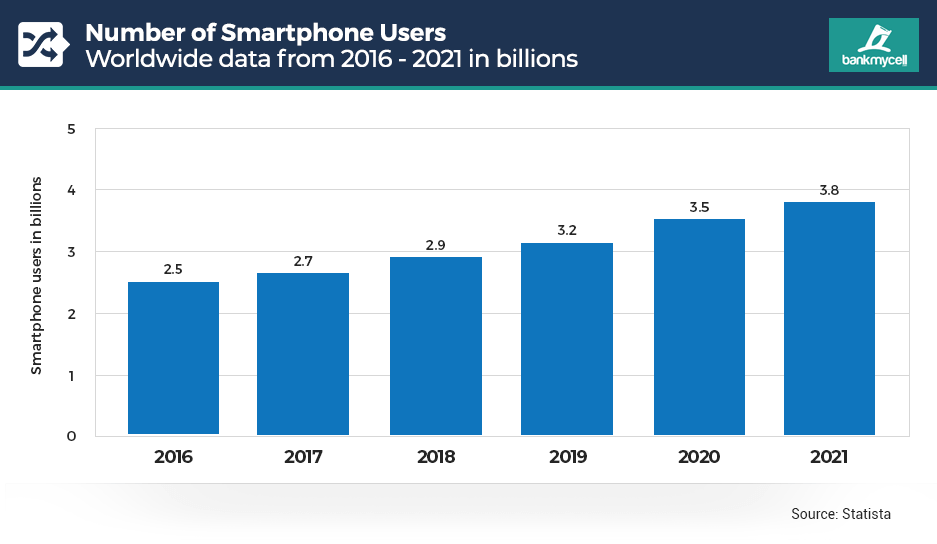
\includegraphics[width=\textwidth]{img/smartphone_users}
\caption{Numero di utilizzatori di smartphone nel mondo \cite{bankmycell}}
\label{fig:smartphone_users}
\end{figure}

\section{mHealth}
Lo sviluppo di questi studi e la diffusione degli smartphone nel mondo ha portato a quella che è chiamata \textbf{mHealth} \textit{(o mobile health)}; la messa in pratica della medicina e della salute pubblica supportata dall'utilizzo di dispositivi mobile\cite{mHealth}.
La mHealth è una parte di quella che viene chiamata \textbf{eHealth}, ovvero l'utilizzo di dispositivi informatici e tecnologici \textit{(dai computer ai monitor dei pazienti)} per il supporto dei servizi salutari.
Questo tipo di tecnologie permette oggi anche a paesi sottosviluppati di avere accesso ad una assistenza sanitaria di qualche tipo per permettere di identificare e curare in tempo eventuali disturbi.

Tra i vari servizi resi disponibili dalla mHealth ci sono anche quelli \textbf{educativi} del paziente sui disturbi di cui soffre, quelli di \textbf{helpline} che forniscono al paziente un contatto con esperti del settore e quelli di \textbf{remote disease surveillance} che permettono al paziente di diventare consapevole dei propri disturbi ed eventualmente sostenere un percorso di guarigione \textit{(che sia online o meno)}, che è esattamente quello a cui miriamo con la nostra applicazione.

\section{Strategie Principali}
Come abbiamo detto, il vantaggio principale delle pratiche come mHealth sono l'accesso in
maniera anonima e la libera scelta di un orario, fattori sicuramente positivi per il target d'udienza dell'applicazione, ovvero gli studenti universitari.
Per quanto riguarda l'identificazione e lo sviluppo di cura dei disturbi psichici, alcune strategie chiave sono il \textbf{monitoraggio dell'umore} del soggetto, la raccomandazione di \textbf{attività che scoraggino i pensieri negativi}, l'\textbf{educazione} del soggetto sui propri disturbi e l'\textbf{accesso alle reti di supporto} da parte di esso; tutte queste strategie fanno parte della \textbf{Terapia Cognitivo-Comportamentale} \cite{CBT} che è un metodo di cura adatto al trattamento individuale ed è finalizzata a trattare i pensieri negativi, le emozioni disfunzionali e i comportamenti disadattivi del paziente in modo da facilitare l'eliminazione dei disturbi psicologici.

\section{Funzionalità Offerte}
Dunque, scopo finale dello stage è stato quello di realizzare un'applicazione di mHealth che permetta agli utenti, nel nostro caso agli studenti universitari, di auto-educarsi sui disturbi di cui potrebbero soffrire tramite un'attività iniziale di \textbf{screening} atta ad identificare segnali d'allarme che possano suggerire la presenza di tali disturbi, e l'eventuale \textbf{educazione} e \textbf{mitigazione} di essi tramite attività di monitoraggio dell'umore, \textbf{lezioni didattiche} sui propri disturbi e su come combatterli, \textbf{esercizi attivi} per il recupero.
Questo sarà eseguito utilizzando dei questionari accompagnati da contenuti multimediali da
completare settimanalmente, uniti a una parte di domande giornaliere per il monitoraggio
dell'utente. I questionari sono creati sulla piattaforma \textbf{Qualtrics}, nata inizialmente per gestire dei questionari di tipo aziendale, che permette di definire diversi tipi di domande e di inserire vari media nelle domande stesse, offrendo l'accesso a tutto ciò tramite API.
Verrà inoltre tenuta traccia dei progressi dell'utente e, utilizzando un calendario, verranno segnalati nuovi esercizi ogni volta che questi sono disponibili. Per permettere un monitoraggio del soggetto sono inoltre disponibili delle domande giornaliere che verranno notificate all'utente ad un orario a sua scelta.


\chapter{Progettazione}
Prima di poter mettere mano all'applicazione è stato necessario un iniziale periodo di studio dell'ambiente, in particolare del linguaggio \textbf{Dart} e del framework \textbf{Flutter}; è stato piacevole scoprire come Flutter supporti nativamente sia il \textbf{Material Design}, stile adottato per lo sviluppo dell'interfaccia grafica \textit{(almeno per quanto riguarda Android)}, sia lo stile \textbf{Cupertino}, ovvero lo stile nativo di iOS, impostando di default alcune regole di tali stili quando vengono creati determinati widget.

Successivamente a questo periodo di studio è iniziata la vera e propria progettazione dell'applicazione, fase durante la quale sono stati stabiliti il modello dei dati e l'architettura adottata per lo sviluppo.

\section{Prima di Qualtrics}
Inizialmente non era stato scelto uno specifico backend, per cui lo sviluppo del modello dati è stato eseguito pensando ad un generale database e ad una generica applicazione che facesse uso di domande e risposte. Come possiamo osservare nella Figura \ref{fig:modello_iniziale}, è stato pensato ad un modello estremamente semplice ma estendibile e che, per il momento, distingueva solo domande a risposta aperta, domande a risposta chiusa e domande \textit{"speciali"} di screening (che inizialmente pensavamo fossero solo a risposta chiusa).
Ad ogni domanda erano poi associate delle opzioni selezionabili \textit{(o definibili nel caso di domande a risposta aperta)} e la risposta ad una certa domanda non era altro che l'opzione \textit{(o le opzioni)} selezionata.

\begin{figure}
\centering
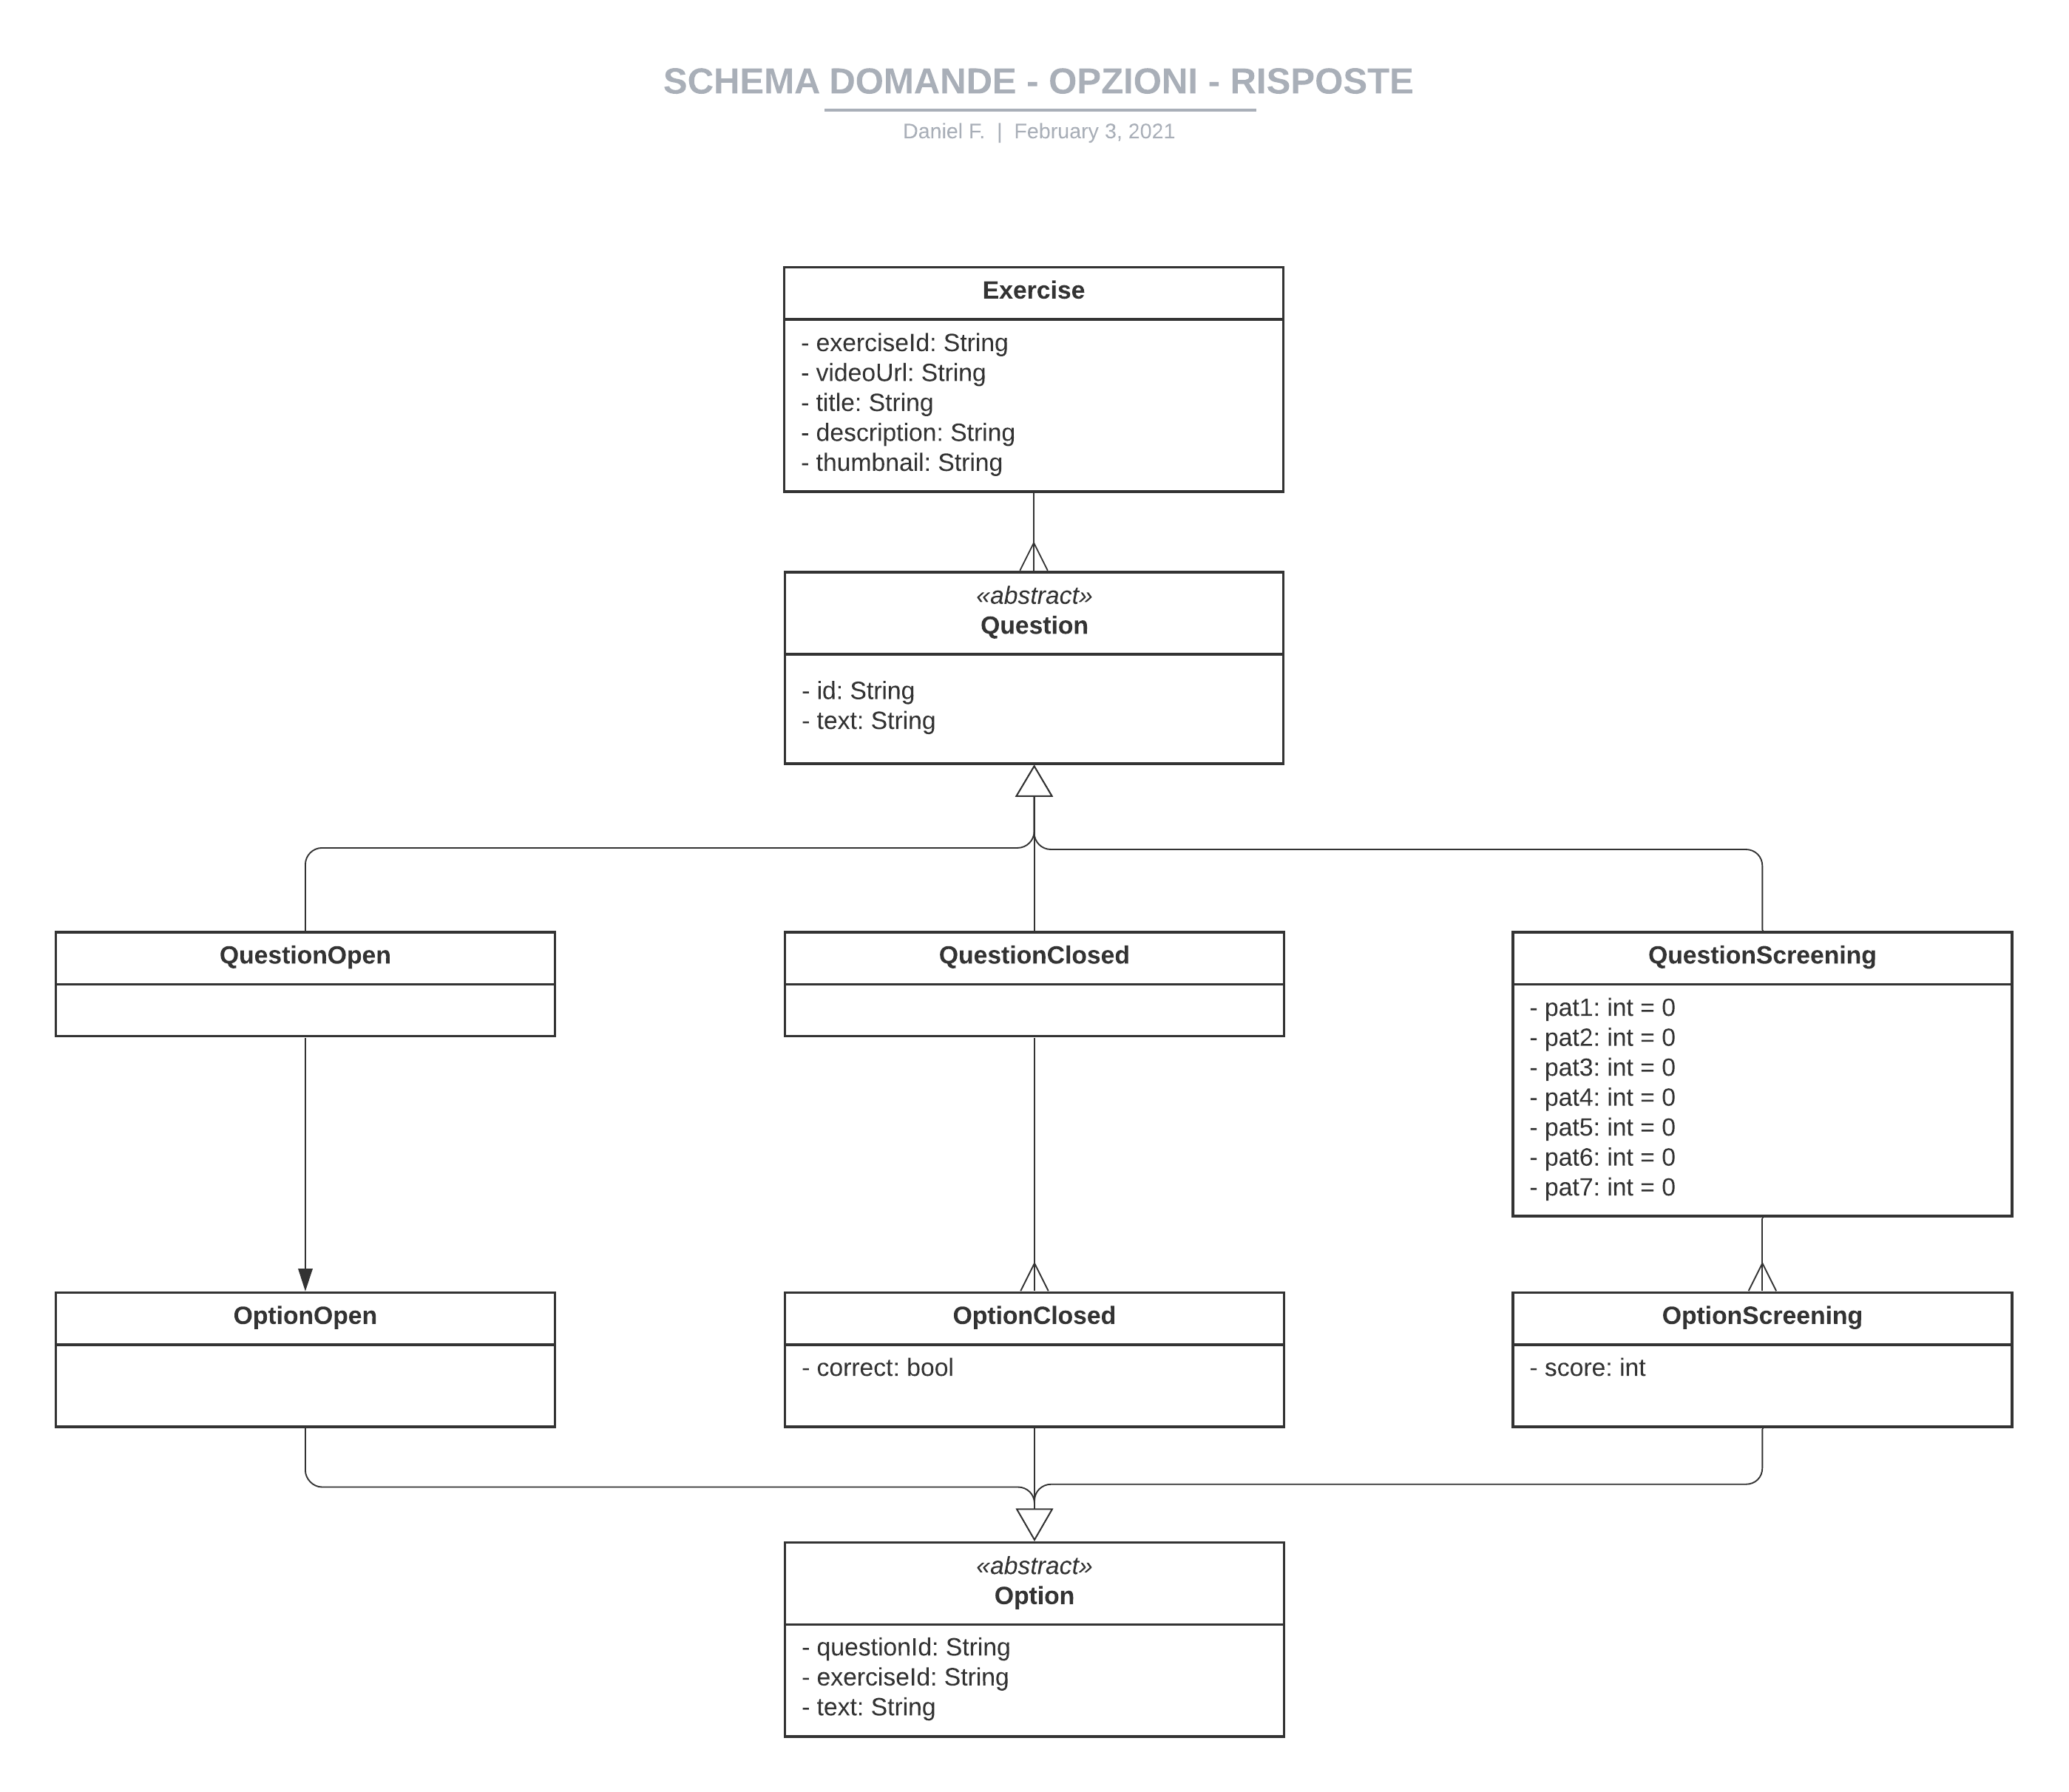
\includegraphics[width=\textwidth]{img/modello_iniziale}
\caption{Modello dati prima di Qualtrics}
\label{fig:modello_iniziale}
\end{figure}

\section{Dopo Qualtrics}
Non molto dopo i primi sviluppi è stato deciso di utilizzare \textbf{Qualtrics}\footnote{\url{www.qualtrics.com/uk/core-xm/survey-software}} come effettivo backend dell'applicazione, che non è altro che una piattaforma di creazione di sondaggi orientata alle aziende per ottenere feedback sia dai propri clienti che dai propri impiegati: l'idea era adattare questo software già pronto e che presenta già diversi tipi di domande utili al nostro scopo per poter ottenere gli input necessari dai nostri utenti e presentarli a chi di dovere. Non solo, essendo una piattaforma a sé stante, essa permette anche al gruppo di psicologia di creare i sondaggi necessari indipendentemente dallo sviluppo dell'applicazione, che si limita, tramite le API di Qualtrics, a ottenere e presentare questi sondaggi.

\subsection{Modello dati: domande}
In particolare, come possiamo vedere nel modello semplificato della Figura \ref{fig:modello_semplice_qualtrics}, il modello dati adottato da Qualtrics prevede un oggetto esterno, la \textbf{Survey} \textit{(sondaggio)}, che contiene, oltre a vari parametri di configurazione, una lista di \textbf{Questions} \textit{(domande, che sono degli oggetti anch'esse)} che possono essere di vario tipo; le domande a loro volta contengono i loro parametri di configurazione ed una lista di possibili risposte \textit{(Choices)} se a risposta chiusa.
Tra i valori interessanti contenuti nei parametri delle domande ci sono il \texttt{QuestionText}, che rappresenta la domanda vera e propria in linguaggio naturale, il \texttt{Selector} che permette di avere domande simili ma differenziate per qualche dettaglio \textit{(ad esempio possiamo avere una domanda a risposta chiusa in cui si possono selezionare più risposte piuttosto che solo una)} e il \texttt{ChoiceOrder}, che stabilisce in che ordine devono apparire le possibili risposte, contenute nell'oggetto \texttt{Choices}.
Ogni entità è inoltre opportunamente identificata, difatti le risposte non sono altro che delle coppie \texttt{<ID\_Domanda, ID\_Risposta>} oppure \texttt{<ID\_Domanda, [ID\_Risposta\_1, ..., ID\_Risposta\_n]>}, nel caso di domande a risposta chiusa, mentre nel caso di domande a risposta aperta sono del tipo \texttt{<ID\_Domanda, "Risposta">}.

\newpage

\subsection{Modello dati: blocchi}
Un aspetto particolare riguardo l'organizzazione delle domande nell'ambiente Qualtrics è quello legato ai \textbf{Blocks}, che sono degli insiemi di domande presentati separatamente. Questo permette di non sovraccaricare una schermata di domande ma di suddividerle in parti visualizzate indipendentemente.
Come si può vedere sempre nella Figura \ref{fig:modello_semplice_qualtrics}, i blocchi sono degli oggetti contenuti nell'oggetto \texttt{Survey} che dispongono di un \texttt{BlockID} e di una \texttt{Description}, una descrizione testuale utilizzata per dare un'idea del contesto delle domande presenti nel blocco. Inoltre, i blocchi contengono una lista di oggetti \texttt{BlockElements} che, seppur contente oggetti, non contiene le domande vere e proprie, ma solo gli \texttt{QuestionID} delle domande facenti parte del rispettivo blocco; è necessario quindi un incrocio dei dati nell'applicazione per far sì che le domande rispettino l'ordine dei blocchi.

È presente inoltre, sempre nell'oggetto\texttt{Survey}, un ulteriore oggetto \texttt{SurveyFlow} che contiene l'ordine di visualizzazione dei blocchi in una lista contenente i \texttt{BlockID} corrispondenti \textit{(in quanto potrebbero non essere nel giusto ordine all'interno dell'oggetto \texttt{Blocks})}.

\begin{figure}
\centering
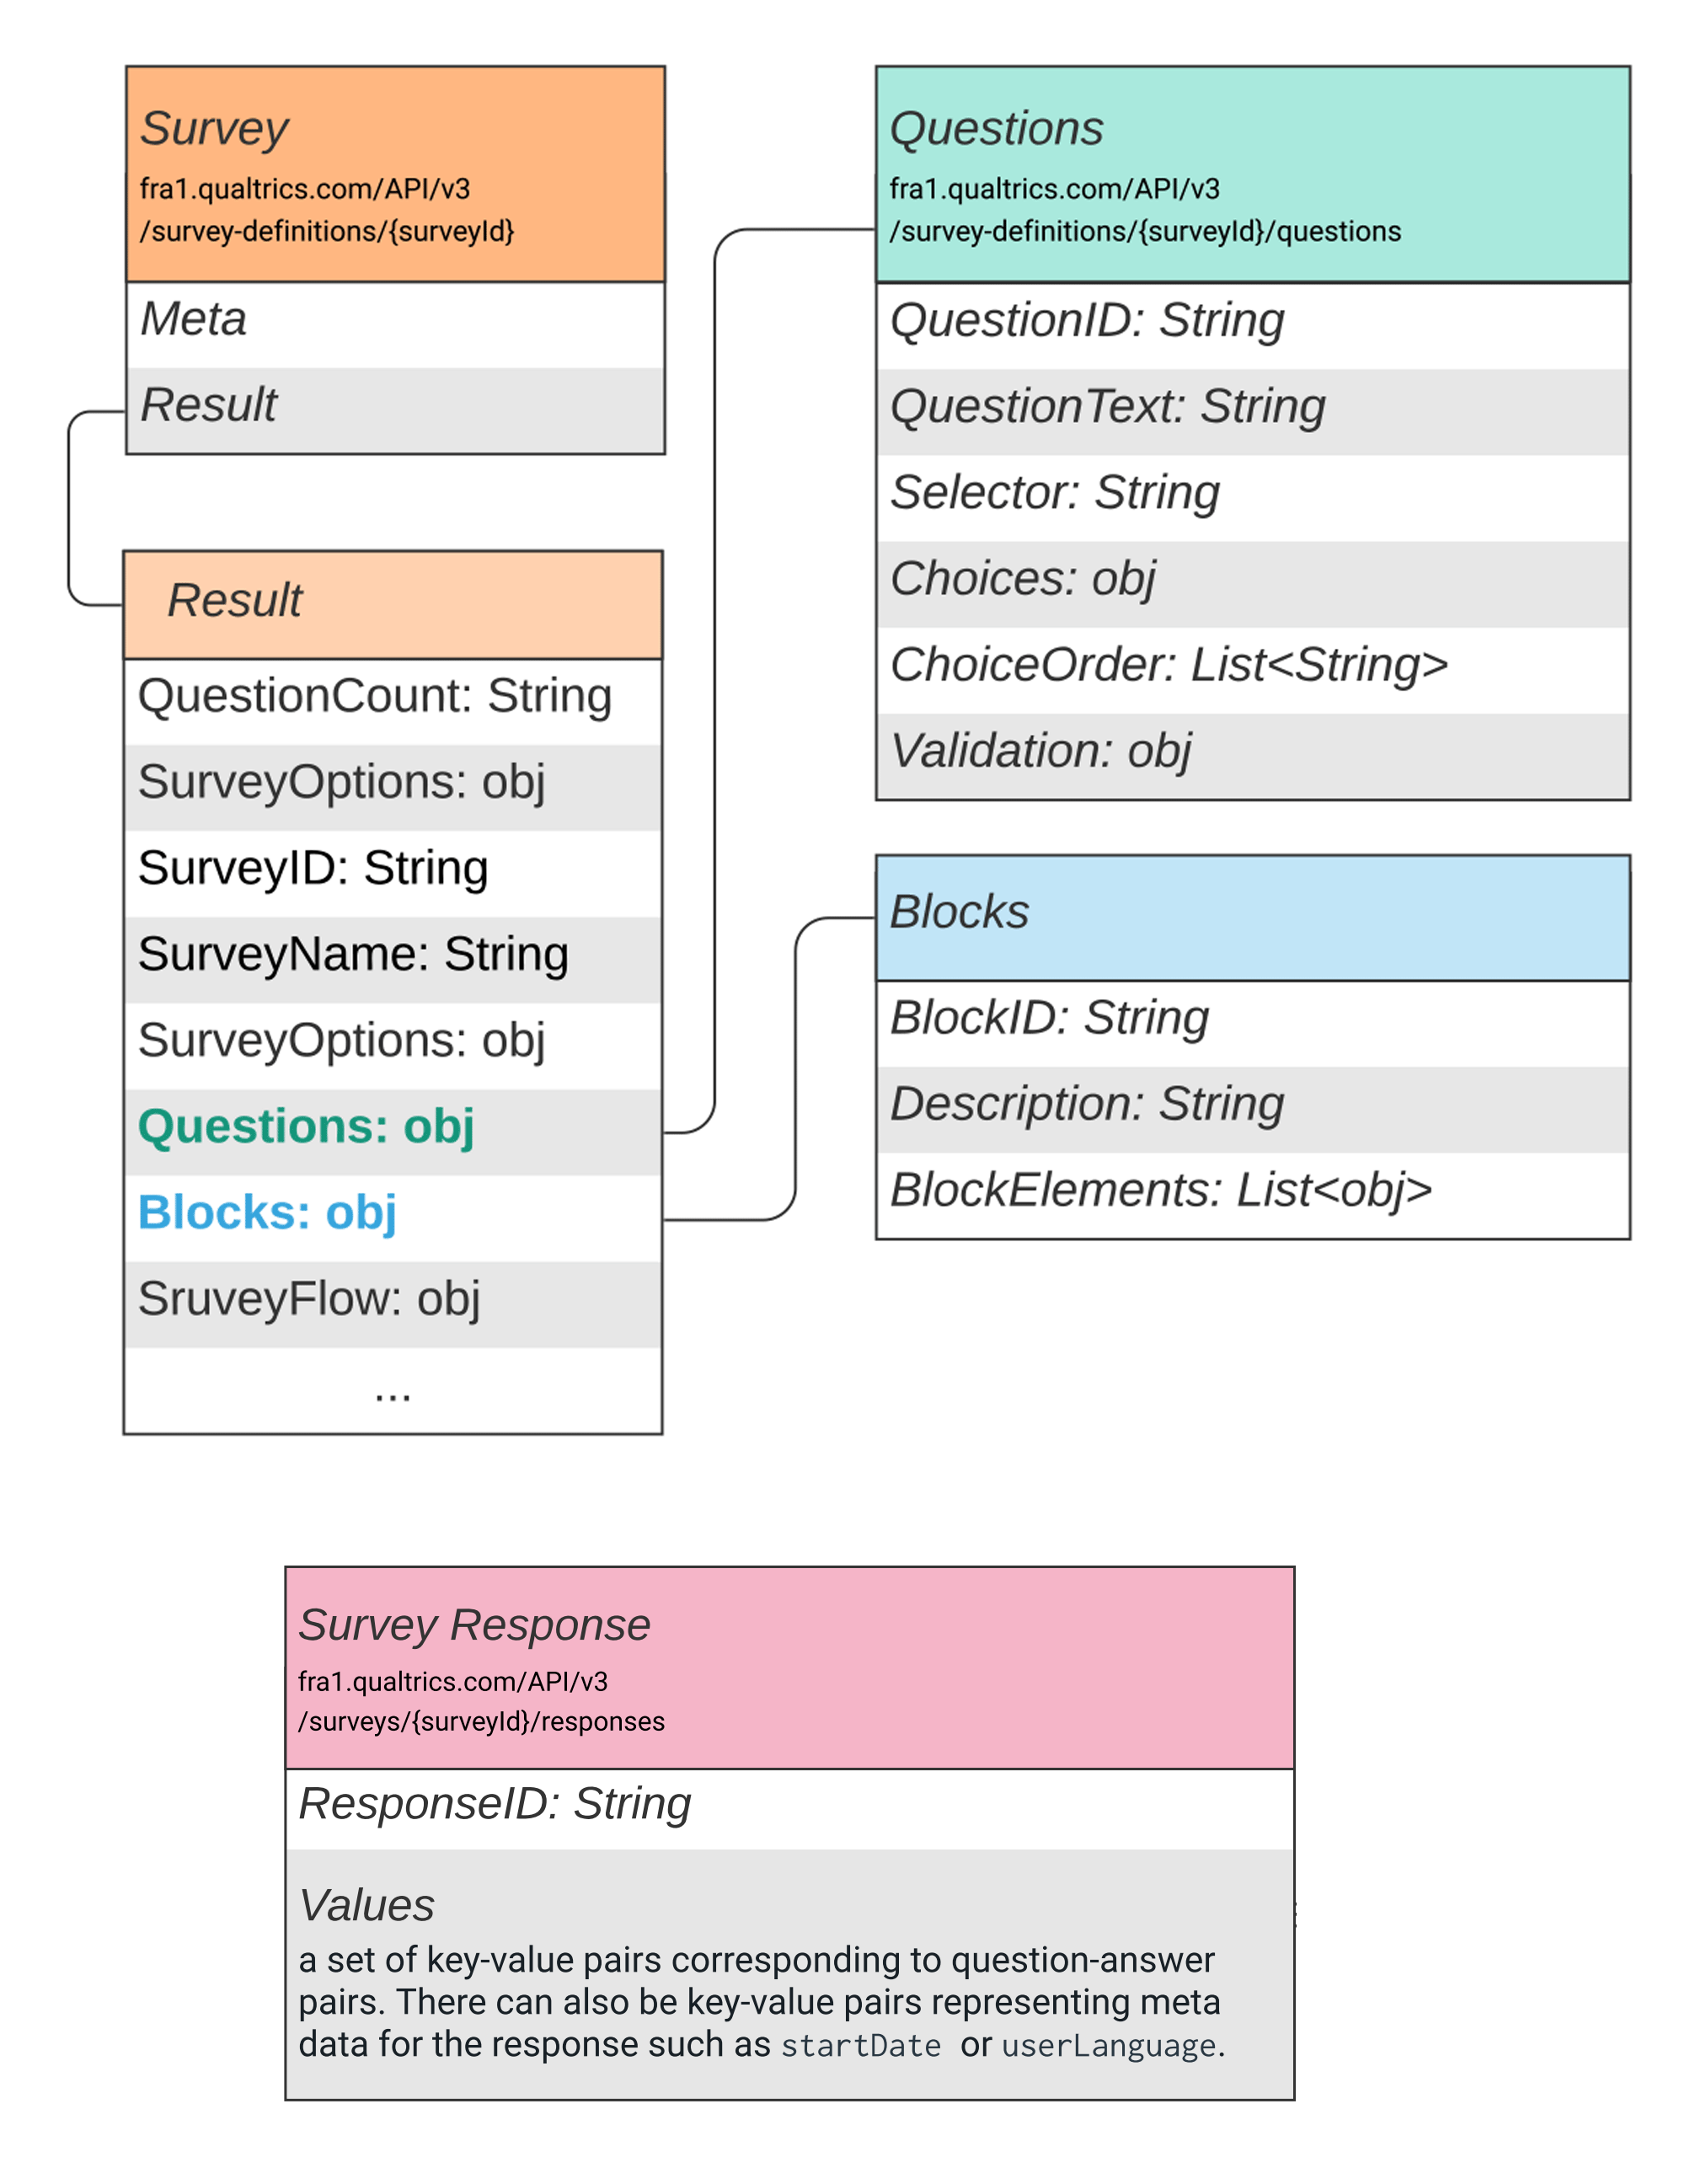
\includegraphics[width=\textwidth]{img/modello_semplice_qualtrics}
\caption{Modello dati Qualtrics semplificato}
\label{fig:modello_semplice_qualtrics}
\end{figure}
\chapter{Implementazione}
Dopo la fase di progettazione è stato possibile creare i primi componenti software ed interfacciarsi col backend di Qualtrics. In particolare è stata spesa buona parte del tempo per studiare i dati che fornisce Qualtrics tramite le sue API per poterli poi adattare ad un contesto mobile e alla creazione di custom widget che consumassero tali dati e li presentassero all'utente.

\section{Endpoint utilizzati}
La prima fase di studio si è concentrata nell'identificare quali chiamate sarebbero state necessarie per il funzionamento dell'applicazione; sono state necessarie varie chiamate per l'autenticazione al servizio di Qualtrics, per recuperare le domande e per inviare le risposte. Inoltre, alcune chiamate sono state utilizzate solo a scopo di test poiché Qualtrics restituisce già tutti i dati necessari per un determinato questionario in un'unica chiamata, seppur in una maniera poco leggibile; effettuare chiamate specifiche per reperire le domande e le informazioni di un determinato blocco permette di avere gli stessi dati in maniera più leggibile. Queste chiamate sono state necessarie \textit{(seppur non implementate nell'applicazione)} poiché purtroppo la documentazione di Qualtrics non fornisce dettagli sulla struttura dei dati delle varie domande e delle risposte; tramite queste chiamate è stato possibile effettuare una sorta di reverse engineering di questi dati.
Possiamo vedere un elenco riassuntivo delle chiamate interessanti nella \autoref{table:api}.

\begin{table}[ht!]
\def\arraystretch{1.5}
\begin{tabular}{| m{3em} | m{12em} | m{17em} |}
 \hline
 \textbf{TIPO} & \textbf{ENDPOINT} & \textbf{DESCRIZIONE} \\
 \hline \hline
 
 POST & /oauth2/token & Restituisce un token Oauth2 con determinati permessi che possa autenticare le chiamate future. \\ 
 \hline
 
 GET & /surveys & Restituisce tutti i questionari presenti nell'ambiente Qualtrics. \\
 \hline
 
 GET & /survey-definitions\newline / \textbf{\{\{surveyID\}\}} & Restituisce i dati completi relativi al questionario \textbf{\{\{surveyID\}\}} come il numero di domande, i blocchi, meta-dati per la visualizzazione web, le domande e i blocchi \textit{(seppur in maniera poco leggibile)}. \\
 \hline
 
 GET & /survey-definitions\newline /\textbf{\{\{surveyID\}\}}/questions & Restituisce tutte le domande del questionario \textbf{\{\{surveyID\}\}} \textit{(senza distinzione fra blocchi)} sotto forma di lista di oggetti e senza ulteriori meta-dati legati alla survey, rendendo i dati molto più leggibili. Questa è una delle chiamate eseguite solo in fase di test ed è stata utilizzata unicamente per osservare e studiare il formato dei dati delle varie domande tramite Postman. \\
 \hline
 
 GET &
 /survey-definitions\newline /\textbf{\{\{surveyID\}\}}\newline /\textbf{\{\{blockID\}\}} &
 Restituisce i dati relativi al blocco\newline \textbf{\{\{blockID\}\}}, tra i quali anche gli ID delle domande facenti parte di quel blocco. Anche questa chiamata è stata utilizzata unicamente a scopo di test. \\
 \hline

 POST & /survey-definitions\newline /\textbf{\{\{surveyID\}\}}/responses & Invia le risposte al questionario \textbf{\{\{surveyID\}\}} al server. \\
 \hline
 
\end{tabular}
\caption{Elenco riassuntivo chiamate API}
\label{table:api}
\end{table}

\textbf{Nota}: il punto di accesso alle API è \texttt{fra1.qualtrics.com/API/v3}, dove \texttt{fra1} è l'identificativo del data center europeo di Qualtrics.

\newpage

\subsection{Autenticazione}
Prima di poter fare qualsiasi tipo di chiamata alle API di Qualtrics è necessario ottenere un token di autenticazione: in particolare Qualtrics permette di ottenere una chiave API direttamente dall'ambiente di creazione dei sondaggi \textit{(meno sicura in quanto offre tutti i permessi a chi ne è in possesso)} oppure di richiedere, tramite la chiamata \texttt{POST fra1.qualtrics.com/oauth2/token}\footnote{\url{api.qualtrics.com/guides/docs/Instructions/oauth-authentication.md}} un \textbf{bearer token}, molto più sicuro di una chiave in quanto è possibile definire per esso solo determinati permessi \textit{(nel nostro caso serviranno solo i permessi per leggere i sondaggi e per scrivere le risposte)}.
Per richiedere tale token è necessario specificare nel campo \texttt{Authentication} della richiesta un \texttt{ClientID} ed un \texttt{ClientSecret}, entrambi generabili dall'ambiente Qualtrics ai quali verranno poi effettivamente assegnati i permessi necessari, mentre nel campo \texttt{Body} sarà necessario specificare il tipo di autenticazione e gli scope richiesti per il token tramite i parametri \texttt{grant\_type=client\_credentials\&scope=\{scope\}}. È interessante notare che è possibile richiedere solo un sottoinsieme di scope disponibili per la coppia <\texttt{ClientID}, \texttt{ClientSecret}>.

Possiamo vedere com'è fatta la risposta a questa chiamata nel \autoref{json:token-res}.

\begin{json}
\usemintedstyle[JSON]{trac}
\begin{minted}[]{JSON}
{
	"access_token": "xxxxxxxx-xxxx-xxxx-xxxx-xxxxxxxxxxxx",
	"token_type": "Bearer",
	"expires_in": 3599,
	"scope": "read:surveys"
}
\end{minted}
\caption{Risposta a chiamata /oauth2/token}
\label{json:token-res}
\end{json}

Una volta ottenuta tale risposta è possibile usare il bearer token presente nel campo \texttt{access\_token} nel campo \texttt{Authentication} delle future richieste per autenticarle.

\textbf{Nota}: com'è possibile vedere anche nella risposta stessa, il bearer token ha una durata limitata nel tempo e scade in un'ora. Quando il token scade sarà necessario dunque richiederne uno nuovo.

\newpage
\subsection{Sondaggi}
A questo punto è possibile consumare effettivamente i dati forniti dalle API di Qualtrics e per far ciò un buon punto di partenza è recuperare i dati relativi ai sondaggi disponibili nello spazio di lavoro di Qualtrics tramite la chiamata \\ \texttt{GET fra1.qualtrics.com/API/v3/surveys} che restituisce una lista di oggetti, ognuno dei quali rappresenta un sondaggio. Possiamo vedere un esempio semplificato di risposta a tale chiamata nel \autoref{json:surveys} \textit{(in cui è riportato solo un sondaggio senza ulteriori meta-dati per semplicità)}, in particolare notiamo che i parametri che ci interessano maggiormente sono il campo \texttt{id}, tramite il quale potremmo ottenere ulteriori informazioni sul sondaggio \textit{(come le sue domande)} e il campo \texttt{name}.

\begin{json}
\usemintedstyle[JSON]{trac}
\begin{minted}[]{JSON}
{
    "result": {
        "elements": [
            {
                "id": "SV_xxxxxxxxxxxxxxx",
                "name": "nome_sondaggio",
                "ownerId": "UR_xxxxxxxxxxxxxxx",
                "lastModified": "2021-06-29T16:34:06Z",
                "creationDate": "2021-04-08T19:40:33Z",
                "isActive": true
            },
        ],
}
\end{minted}
\caption{Risposta a chiamata /surveys}
\label{json:surveys}
\end{json}

\newpage
\subsection{Sondaggio: domande, blocchi e flow}
Usando gli id restituiti dalla prima chiamata possiamo a questo punto ottenere ulteriori informazioni su ogni sondaggio tramite la chiamata \\ \texttt{GET fra1.qualtrics.com/API/v3/survey-definitions/\{\{surveyID\}\}}.
In particolare, come è possibile osservare nel \autoref{json:surveyID} questa chiamata ci fornirà informazioni più dettagliate sul sondaggio come il numero di domande, i blocchi presenti nel sondaggio e il \texttt{SurveyFlow}, ovvero l'ordine dei blocchi.

\vskip 5em
\subsubsection{Domande}
Si può notare che questa chiamata ci fornisce già anche le domande; nell'applicazione, per questione di ottimizzazione di dati e chiamate, viene effettivamente fatta solo questa chiamata per impostare un determinato sondaggio. La particolarità però è che questa chiamata fornisce le domande come un oggetto con all'interno altri oggetti \textit{(le domande stesse)}, il tutto corredato con i dati specifici al questionario stesso: essendo le domande anch'esse degli oggetti relativamente complessi \textit{(non sono mostrate in questo esempio perché ne parleremo dopo distinguendole per tipo)}, può risultare difficile per una persona leggere questi dati, anche se un programma non ha questo problema.

Come detto prima, per risolvere questo inconveniente è stata usata la chiamata \texttt{GET /survey-definitions/\{\{surveyID\}\}/questions} che restituisce solo una lista con gli oggetti rappresentanti le domande, molto più facile da leggere per capire quali parametri servono per implementare la domanda stessa.
Discorso analogo vale anche per i blocchi che sono già forniti in questa chiamata e che possono essere ottenuti in un formato più leggibile tramite la chiamata \texttt{GET /survey-definitions/\{\{surveyID\}\}/\{\{blockID\}\}}.

Anche in questo caso il JSON di esempio riportato è semplificato; sono stati omessi alcuni campi che non vengono utilizzati in ogni caso dall'applicazione.

\newpage
\begin{json}
\usemintedstyle[JSON]{trac}
\begin{minted}[]{JSON}
{
    "result": {
        "QuestionCount": "246",
        "SurveyID": "SV_xxxxxxxxxxxxxxx",
        "Questions": { "*oggetti domande*" }
        "Blocks": {
            "BL_xxxxxxxxxxxxxxx": {
                "Type": "Default",
                "Description": "nome_blocco",
                "ID": "BL_xxxxxxxxxxxxxxx",
                "BlockElements": [
                    {
                        "Type": "Question",
                        "QuestionID": "QID235"
                    }
                ],
            },
            "BL_xxxxxxxxxxxxxxx": {
                "Type": "Trash",
                "Description": "Trash / Unused Questions",
                "ID": "BL_xxxxxxxxxxxxxxx",
                "BlockElements": [],
            },
        "SurveyFlow": {
            "Flow": [
                {
                    "ID": "BL_xxxxxxxxxxxxxx1",
                },
                {
                    "ID": "BL_xxxxxxxxxxxxxx2",
                },
            ],
        },
}
\end{minted}
\caption{Risposta a chiamata /surveys}
\label{json:surveyID}
\end{json}

\subsection{Response}
La chiamata \texttt{POST /survey-definitions/\{\{surveyID\}\}/responses} è, escludendo la chiamata necessaria ad ottenere il bearer token, l'unica chiamata col metodo \texttt{POST} che l'applicazione andrà ad utilizzare per inviare al server di Qualtrics le risposte di un determinato questionario.
Anche in questo caso la documentazione ufficiale di Qualtrics non era molto chiara a proposito di come dovevano effettivamente essere strutturati i dati da inviare, ma è stato tuttavia possibile creare delle risposte di testing e, utilizzando una richiesta \texttt{GET}, recuperare la struttura delle risposte per i diversi tipi di domanda. Possiamo osservare un esempio di risposta nel \autoref{json:response}. Non entriamo nei dettagli delle risposte vere e proprie adesso poiché dipendono dal tipo di domanda e ne parleremo dunque dopo. Notiamo però che ci sono molti meta-dati, tra i quali anche quelli legati alla localizzazione \textit{(ottenuta tramite IP)} che però, al fine di mantenere l'anonimato dei nostri utenti, noi non forniremo considerando che sono opzionali. Quello che verrà effettivamente inviato al server sono delle coppie \texttt{"QuestionID": "Response"} inserite nel campo \texttt{values} \textit{(similmente a quanto detto nella \autoref{subsection:risposte} del capitolo precedente}) senza alcun meta-dato.

\begin{json}
\usemintedstyle[JSON]{trac}
\begin{minted}[]{JSON}
{
    "result": {
        "responseId": "R_xxxxxxxxxxxxxxx",
        "values": {
            "startDate": "2021-07-02T17:59:35Z",
            "endDate": "2021-07-02T17:59:35Z",
            "status": 2,
            "progress": 100,
            "duration": 0,
            "finished": 1,
            "recordedDate": "2021-07-02T17:59:35.863Z",
            "locationLatitude": "45.3197937012",
            "locationLongitude": "8.42129516602",
            "distributionChannel": "test",
        }
    }
}
\end{minted}
\caption{Esempio di oggetto response creato automaticamente da Qualtrics}
\label{json:response}
\end{json}

\newpage
\section{Gestione blocchi}
Abbiamo detto che i blocchi sono degli sotto-insiemi di domande da mostrare separatamente: per fare ciò tuttavia sono necessarie alcune operazioni preliminari atte a ordinare i blocchi e successivamente ad associare le domande che essi contengono ai relativi blocchi.

\subsection{Ordine blocchi}
Possiamo notare nel \autoref{json:survey_flow} come l'oggetto \texttt{SurveyFlow} contenga, in ordine di presentazione, gli ID dei blocchi da mostrare. Per rispettare tale ordine è necessario un incrocio di dati: leggendo i dati del campo \texttt{SurveyFlow} possiamo accedere all'oggetto \texttt{Blocks}, di cui possiamo osservare la struttura nel \autoref{json:blocks}, nel giusto ordine, utilizzando il \texttt{BlockID} come chiave di accesso.

\begin{json}
\usemintedstyle[JSON]{trac}
\begin{minted}[]{JSON}
"SurveyFlow": {
   "Flow": [
      {
         "ID": "BL_xxxxxxxxxxxxxx1",
      },
      {
         "ID": "BL_xxxxxxxxxxxxxx2",
      },
   ],
}
\end{minted}
\caption{Oggetto SurveyFlow}
\label{json:survey_flow}
\end{json}

\newpage
\subsection{Domande appartenenti al blocco}
Allo stesso modo possiamo notare nel \autoref{json:blocks} come i blocchi presentino solo l'ID delle domande che contengono ed è quindi nuovamente necessario, come detto anche nella \autoref{subsection:blocchi} del capitolo precedente, incrociare i dati per assegnare poi a livello di applicazione le domande ai relativi blocchi: leggendo il campo \texttt{BlockElements} si accede agli ID delle domande interessate e, utilizzandoli come chiave per accedere all'oggetto \texttt{Questions}, si possono ottenere solo le domande di un determinato blocco.

\begin{json}
\usemintedstyle[JSON]{trac}
\begin{minted}[]{JSON}
"Blocks": {
   "BL_xxxxxxxxxxxxxxx": {
      "Type": "Default",
      "Description": "nome_blocco",
      "ID": "BL_xxxxxxxxxxxxxxx",
      "BlockElements": [
         {
            "Type": "Question",
            "QuestionID": "QID235"
         }
      ],
   },
   "BL_xxxxxxxxxxxxxxx": {
      "Type": "Trash",
      "Description": "Trash / Unused Questions",
      "ID": "BL_xxxxxxxxxxxxxxx",
      "BlockElements": [],
   },
  }
\end{minted}
\caption{Oggetto Blocks}
\label{json:blocks}
\end{json}

\subsection{Trash}
Particolare attenzione va prestata ad uno specifico blocco, ovvero quello con il parametro \texttt{"Type": "Trash"}: questo particolare blocco è il cestino delle domande cancellate dal sondaggio e, se non svuotato, presenterà degli ID di domande che però non devono essere visualizzate. Il modo più semplice per gestire questo blocco è saltarlo direttamente controllando il campo \texttt{Type}.

\section{Memorizzazione dati}
In questa sezione saranno discusse le modalità in cui l'applicazione salva e ordina i dati ottenuti dalle API, in modo da poter poi costruire i widget necessari.

\subsection{Struttura dati}
Le strutture dati scelte per questa applicazione sono le mappe \textit{(o Hash Tables, Hash Maps)}, questo perché abbiamo osservato che ogni entità fornita da Qualtrics è provvista di un ID e, in particolare, generalmente gli ID non seguono un ordine preciso \textit{(fanno eccezione i \texttt{QuestionID} che sono numerati in ordine di creazione, ma creando ed eliminando domande possono presentare comunque salti)}. Essendo poi gli ID univoci conviene sicuramente utilizzare una mappa per salvare i dati, utilizzando gli ID come chiave di ogni entità: in questo modo è possibile accedere velocemente ad una qualsiasi entità salvata utilizzando il suo ID, questo perché l'accesso ai valori di una mappa, conoscendo la chiave, richiede un tempo \textbf{O(1)}, ovvero costante\cite{hashmaps}.
Inoltre, spesso i dati assumono strutture diverse \textit{(ad esempio i diversi tipi di domanda)} e poiché Dart permette, tramite la keyword \texttt{dynamic}, di avere oggetti di tipo diverso come valore di una mappa è sicuramente più semplice utilizzare delle mappe piuttosto che degli array per salvare questi dati.

\subsection{Organizzazione dati}
Per quanto riguarda l'organizzazione dei dati, per semplicità e per come sarebbero poi stati visualizzati i dati, si è scelto di creare una mappa esterna le cui chiavi sono i \texttt{SurveyID} e i valori delle ulteriori mappe che rappresentano i blocchi di ogni sondaggio.

I blocchi, anch'essi delle mappe con chiave il \texttt{BlockID}, contengono a loro volta delle terze mappe, le più interne, che rappresentano le domande e che quindi hanno come chiave il \texttt{QuestionID} e come valore i vari parametri propri a ciascuna domanda.
È stata scelta questa organizzazione dei dati anche perché le domande possono cambiare radicalmente in termini di parametri, quindi definire un tipo specifico per tutte le domande non sarebbe stato possibile. In questo modo inoltre ogni componente accede solo ad un livello dei dati: la pagina che contiene i vari sondaggi accede al primo livello, la pagina principale del sondaggio al secondo e la pagina effettiva delle domande al terzo.

\section{Domande}
In questa sezione saranno analizzati i vari tipi di domande che Qualtrics mette a disposizione, come sono fatte, come sono codificate dalle API e come vengono tradotte nell'applicazione mobile.

\subsection{Text Entry - "QuestionType": "TE"}
La più semplice domanda utilizzabile nel contesto di Qualtrics è la Text Entry: una domanda che mette a disposizione un campo di testo dove scrivere una risposta aperta.
Possiamo osservare la struttura dati semplificata di questo tipo di domande nel \autoref{json:text_entry}. Notiamo in particolare, oltre al \texttt{QuestionText} e al \texttt{QuestionType} che definisce il tipo di domanda, che c'è anche un oggetto \texttt{Validation}: questo oggetto è presente in ogni domanda e serve per definire delle regole secondo le quali una risposta è giusta o meno, ne parleremo in modo più dettagliato successivamente.
Qualtrics permette anche di definire se la risposta dovrebbe essere corta, media o lunga, modificando la dimensione del campo di testo: questa distinzione viene fatta tramite il campo \texttt{Selector} che vale \texttt{"SL"} \textit{(Single Line)} se la risposta è corta, \texttt{"ML"} \textit{(Multi Line)} se è media e \texttt{ESTB} \textit{(Essay Text Box)} se è lunga. Nell'applicazione viene letto questo campo e viene impostata una dimensione rispettivamente di una, 5 o 10 righe del campo di input. È importante notare tuttavia che questo limite non è fortemente restrittivo: seppur la dimensione del campo di input sia limitata, l'utente può comunque inserire una risposta più lunga, si tratta per lo più di una feature di quality of life. Possiamo osservare com'è renderizzata questa domanda rispettivamente nella webview di Qualtrics e nell'applicazione Flutter nella \autoref{fig:text_entry}.

\subsubsection{Response}
La risposta a questo tipo di domande è del tipo\\ \texttt{\{"QuestionID": "testo risposta"\}}, ovvero viene inserita come risposta la stringa stessa inserita dall'utente nel campo di input.

\newpage
\begin{json}
\usemintedstyle[JSON]{trac}
\begin{minted}[]{JSON}
{
        "QuestionText": "testo_domanda",
        "QuestionID": "QID247",
        "QuestionType": "TE",
        "Selector": "SL",
        "Validation": {},
}
\end{minted}
\caption{Oggetto domanda Text Entry}
\label{json:text_entry}
\end{json}

\begin{figure}[h]
\centering
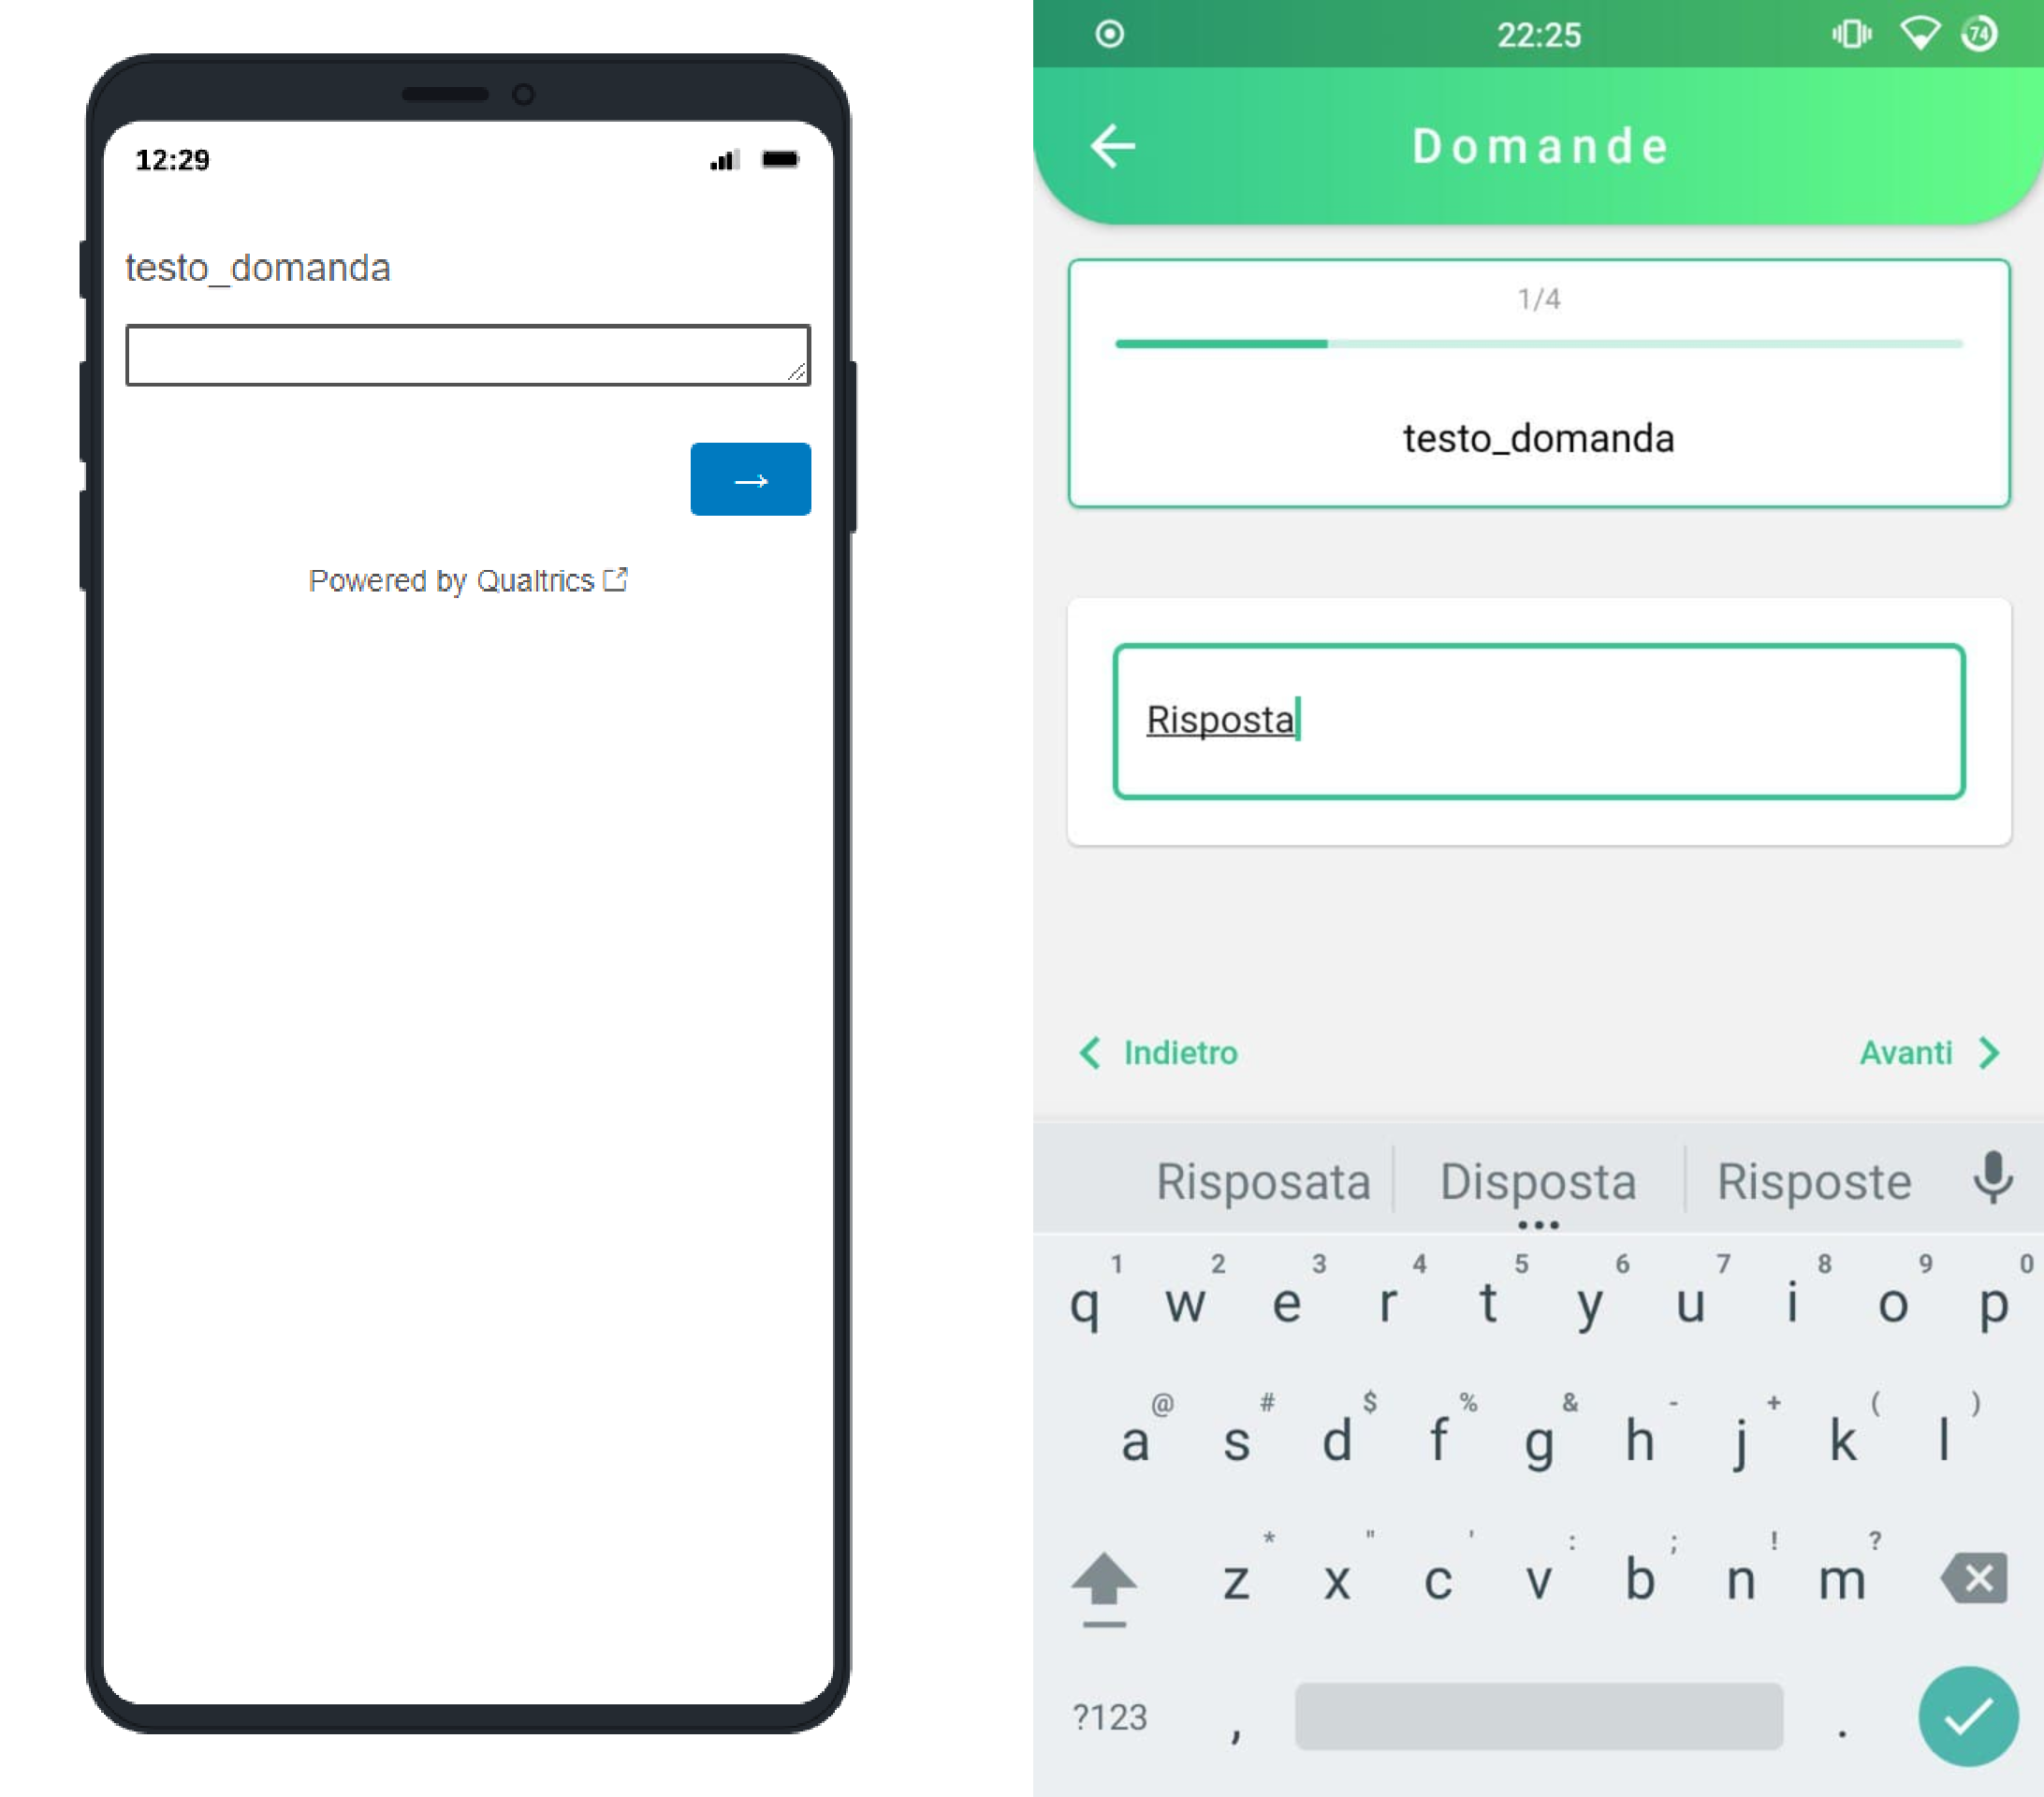
\includegraphics[width=0.7\textwidth]{img/text_entry_flutter}
\caption{Text Entry}
\label{fig:text_entry}
\end{figure}

\newpage
\subsection{Multiple Choice - "QuestionType": "MC"}
Un'altra domanda semplice e che ci si aspetta di trovare in qualsiasi applicazione che faccia uso di questionari è la Multiple Choice: la classica domanda a risposta chiusa che mette a disposizione dell'utente delle risposte predefinite da scegliere. Possiamo osservare la struttura semplificata di questo tipo di domanda nel \autoref{json:mc}. Anche in questo caso Qualtrics mette a disposizione un \texttt{Selector} che però, a differenza di prima, cambia maggiormente la domanda. Questo selettore può essere \texttt{SAVR}, \texttt{SAHR} o \texttt{SACOL} per le domande a risposta singola \textit{(SA = Single Answer)} che, sul web, possono essere visualizzate verticalmente, orizzontalmente o in colonna. Tuttavia nell'applicazione, per questioni di spazio disponibile, le risposte saranno visualizzate sempre verticalmente. Per le domande a risposta singola il selettore può assumere anche il valore \texttt{DL} \textit{(Dropdown List)} che permette di scegliere la risposta tramite un menù a tendina.

Allo stesso modo il selettore può assumere anche i valori \texttt{MAVR}, \texttt{MAHR} e \texttt{MACOL} \textit{(MA = Multiple Answers)} che permette alla domanda di avere più di una risposta scelta, influenzando così anche la risposta generata. Di conseguenza, come possiamo vedere nella \autoref{fig:mc}, in base al \texttt{Selector} l'applicazione costruirà diversi widget: uno per le risposte singole, uno col menù a tendina o uno per le risposte multiple.

Possiamo anche notare che tra i vari dati della domanda ci sono le \texttt{Choices}, ovvero le possibili risposte col proprio testo opportunamente identificate \textit{(notiamo anche che gli ID sono in ordine di creazione, non di presentazione)}. Osserviamo anche il campo \texttt{ChoiceOrder} che contiene gli ID delle choices in ordine di presentazione \textit{(che può essere diverso dall'ordine nel quale sono presenti nel campo \texttt{Choices})}: sarà necessario anche in questo caso incrociare i dati come fatto precedentemente con i blocchi e le domande.

\subsubsection{Media nelle opzioni}
Come abbiamo visto prima, le opzioni di una domanda a risposta chiusa sono di fatto un oggetto: questo perché Qualtrics permette di inserire nelle scelte delle immagini o delle caselle di testo \textit{(per esempio per implementare un'opzione "Altro")} aggiungendo all'oggetto relativo alla Choice interessata rispettivamente i parametri \texttt{"Image": \{\}} \textit{(che conterrà l'url dell'immagine)} e \texttt{"TextEntry": "true"}.
Possiamo osservare un esempio di questo tipo di risposte nella \autoref{fig:mc_media}.

\subsubsection{Response}
La risposta a queste domande è diversa nel caso di risposta singola e nel caso di risposte multiple: se la domanda accetta solo una risposta è del tipo \texttt{\{"QuestionID": ChoiceID\}}, ovvero è l'ID della risposta scelta reperibile dal campo \texttt{Choices} \textit{(notare l'assenza di apici)}, mentre se la domanda accetta risposte multiple è del tipo \texttt{\{"QuestionID": ["ChoiceID\_1", "ChoiceID\_2"]\}}, ovvero una lista con gli ID delle risposte scelte. Se l'opzione scelta contiene una text entry inoltre, nella risposta sarà presente anche il campo \texttt{"QuestionID\_TEXT": "testo risposta"}.

\begin{json}
\usemintedstyle[JSON]{trac}
\begin{minted}[]{JSON}
{
    "QuestionText": "testo_domanda",
    "QuestionID": "QID247",
    "QuestionType": "MC",
    "Selector": "SAVR",
    "Choices": {
        "4": {
            "Display": "Risposta 1"
        },
        "5": {
            "Display": "Risposta 2"
        },
        "6": {
            "Display": "Risposta 3"
        }
    },
    "ChoiceOrder": [
        "4",
        "5",
        "6"
    ],
    "Validation": {},
}
\end{minted}
\caption{Oggetto domanda Multiple Choice}
\label{json:mc}
\end{json}

\begin{figure}[ht!]
\centering
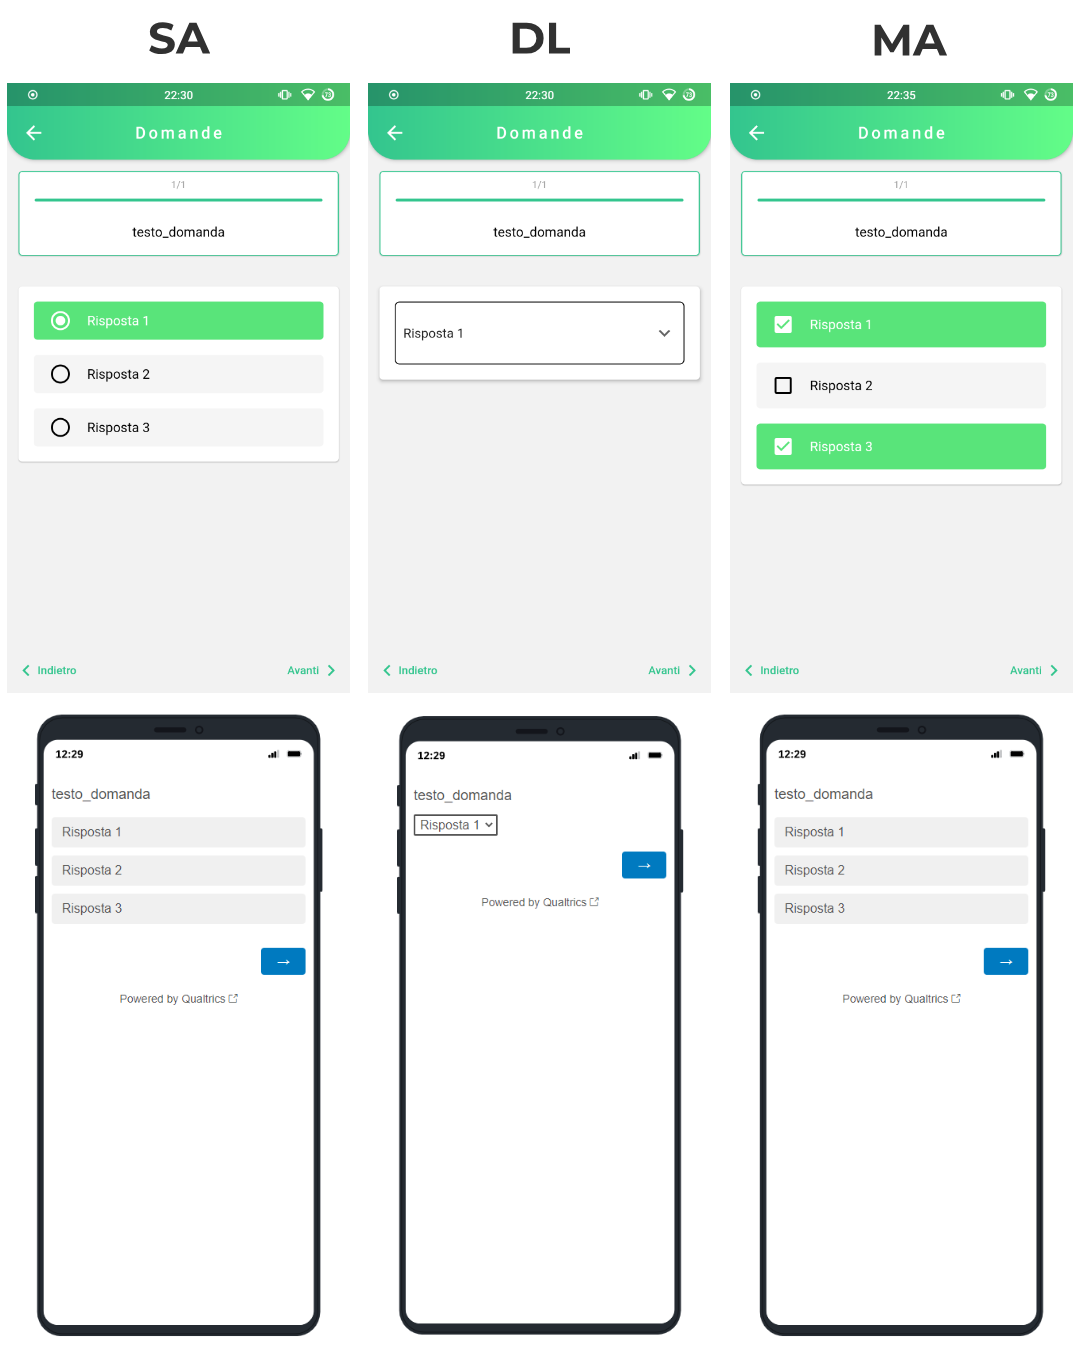
\includegraphics[width=\textwidth]{img/mc_flutter}
\caption{Multiple Choices}
\label{fig:mc}
\end{figure}

\begin{figure}[ht!]
\centering
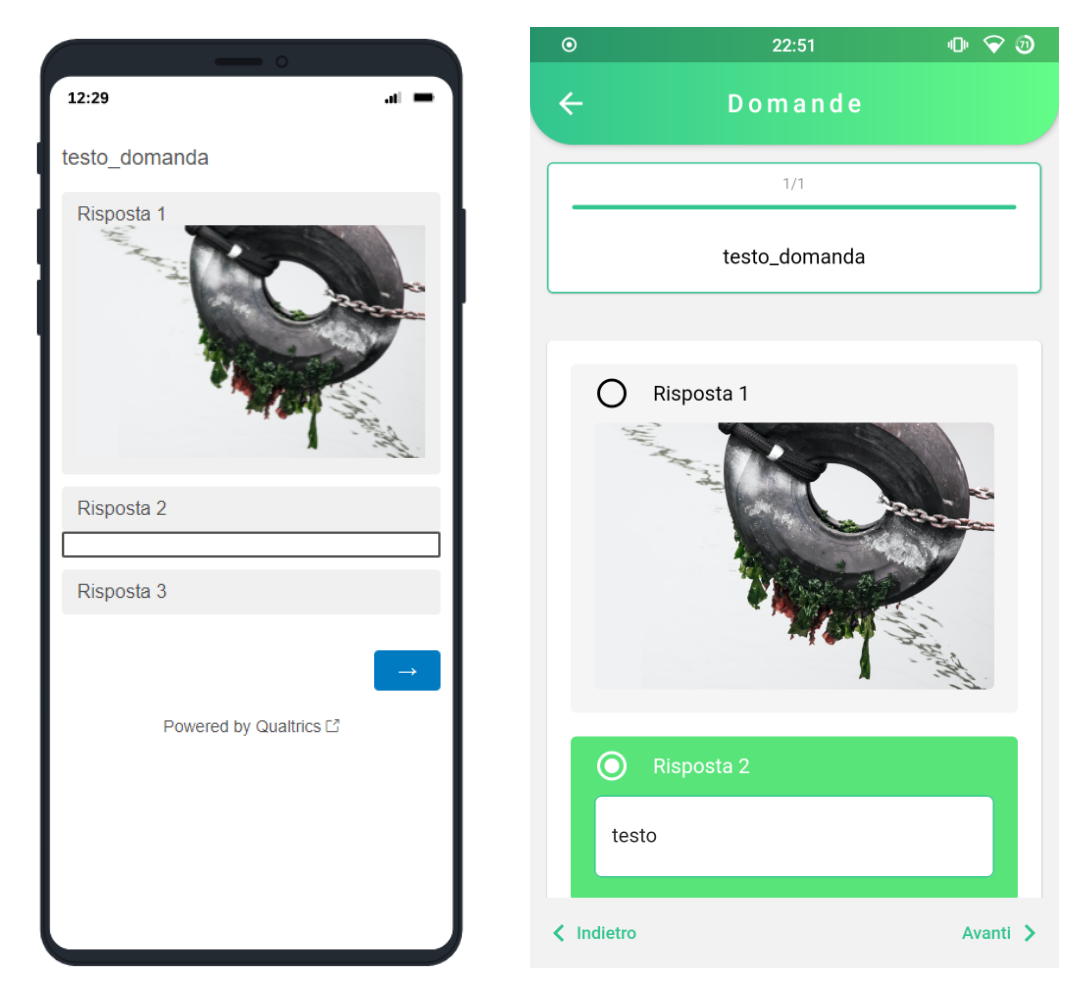
\includegraphics[width=0.7\textwidth]{img/mc_media}
\caption{Domanda con media e text entry nelle opzioni}
\label{fig:mc_media}
\end{figure}

\clearpage
\subsection{NPS - "QuestionType": "MC"}
Un tipo particolare di domanda Multiple Choice che viene però trattato da Qualtrics come un tipo separato è il \textbf{Net Promoter Score}, una domanda che richiede di assegnare un punteggio da 0 a 10 a un qualcosa. Possiamo osservarne la struttura nel \autoref{json:nps} e notiamo che quello che la distingue dalle altre domande di tipo MC è il \texttt{Selector} di tipo \texttt{NPS}, e che contiene delle label nel campo \texttt{ColumnLabels} utili a dare un'idea del giudizio che si sta dando. Possiamo osservare un esempio di questa domanda nella \autoref{fig:nps}.

\subsubsection{Response}
La risposta a questo tipo di domanda è del tipo \texttt{\{"QuestionID": numero\}}.

\begin{json}
\usemintedstyle[JSON]{trac}
\begin{minted}[]{JSON}
{
    "QuestionText": "testo_domanda",
    "QuestionType": "MC",
    "Selector": "NPS",
    "Choices": [
        {
            "Display": "0"
        },
        ...
        {
            "Display": "10"
        }
    ],
    "ChoiceOrder": [],
    "ColumnLabels": [
        {
            "Display": "Not at all likely",
        },
        {
            "Display": "Extremely likely",
        }
    ],
            }
\end{minted}
\caption{Oggetto domanda NPS}
\label{json:nps}
\end{json}

\begin{figure}[ht!]
\centering
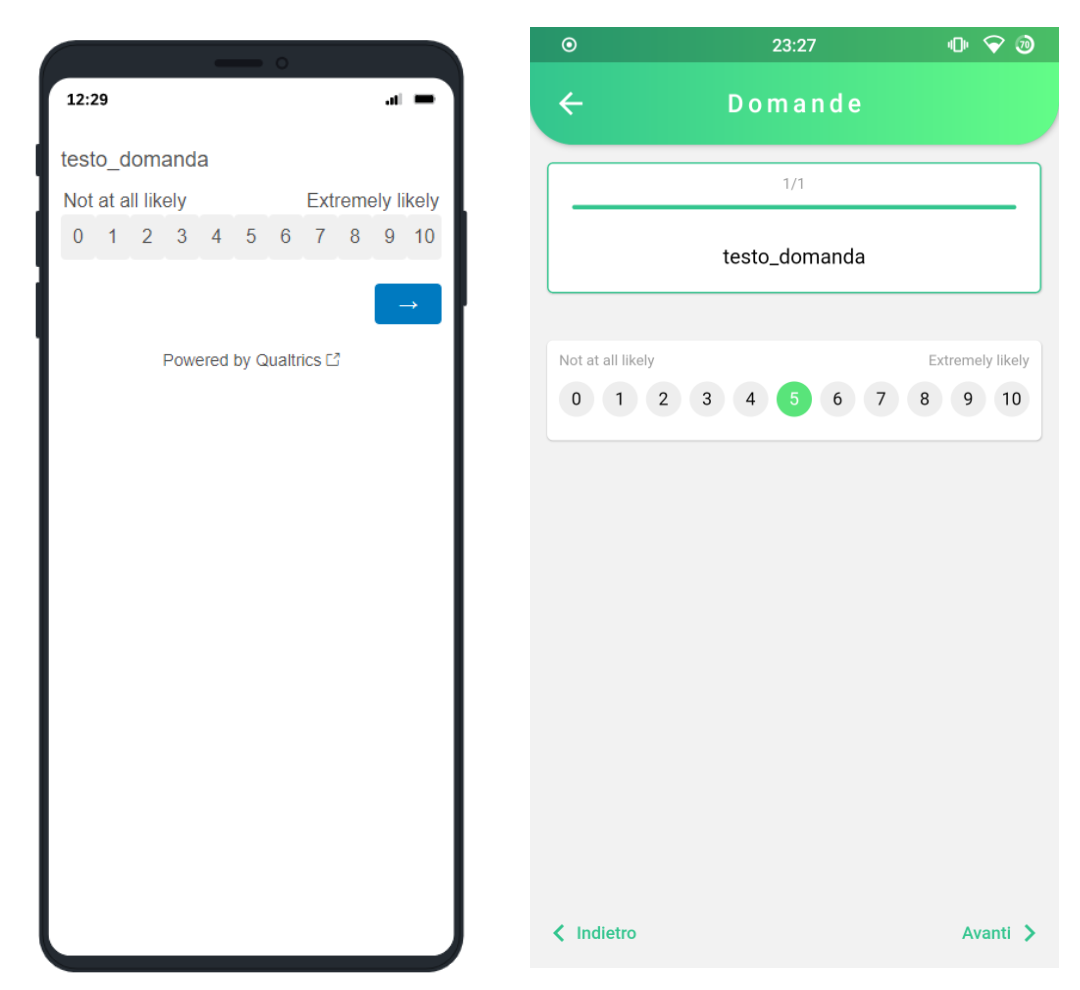
\includegraphics[width=0.7\textwidth]{img/nps}
\caption{Domanda Net Promoter Score}
\label{fig:nps}
\end{figure}

\clearpage
\subsection{Matrix Table - "QuestionType": "Matrix"}
Uno dei tipi più complessi di domanda messi a disposizione da Qualtrics è il tipo Matrix: una serie di diverse domande che però hanno le stesse risposte \textit{(o lo stesso tipo di risposta)}. Questo tipo di domande sono utili per quando sono necessarie più domande che dovrebbero essere valutate su una stessa scala. Possiamo osservare la struttura di queste domande nel \autoref{json:matrix}. Notiamo che, almeno in parte, somiglia molto ad una domanda di tipo Multiple Choices: anche la matrice presenta delle \texttt{Choices} ordinate secondo un \texttt{ChoiceOrder}, ma presenta anche un secondo gruppo di elementi, le \texttt{Answers}, ordinate anch'esse secondo un \texttt{AnswerOrder}.
Possiamo pensare alle \texttt{Choices} come alle risposte vere e proprie, uguali per tutte le domande, e alle \texttt{Answers} come alle domande da valutare \textit{(la scelta dei nomi da parte di Qualtrics non è delle migliori in questo caso)}. Un altro modo per visualizzare il tutto è pensare ad una tabella	dove le \texttt{Choices} identificano le colonne e le \texttt{Answers} le righe \textit{(che è anche il metodo in cui Qualtrics mostra, nella variante web, queste domande)}. Le matrici inoltre, come le NPS, supportano le label.

Nel JSON possiamo anche notare, oltre al "classico" \texttt{Selector} già visto in precedenza, anche un \texttt{SubSelector} che svolge la funzione del \texttt{Selector} di prima, ovvero permette di scegliere il tipo di risposta che la domanda accetta. Mentre il \texttt{Selector} delle matrici serve a cambiare radicalmente il sotto-tipo di domanda: Qualtrics mette a disposizione diversi tipi di matrice, oltre che diversi tipi di risposte per esse.

\subsubsection{Media}
Come per le Multiple Choice, anche in queste domande è possibile inserire delle immagini e delle text entry nelle \texttt{Choices}, mentre per le \texttt{Answers} è possibile solo inserire delle immagini.

\subsubsection{Response}
In questo caso le response sono identificate, oltre che dal \texttt{QuestionID}, anche dal \texttt{ChoiceID}, la chiave difatti è \texttt{QuestionID\_ChoiceID}. La risposta vera e propria tuttavia cambia, oltre che in base al tipo di risposta che accetta la matrice, anche in base al tipo stesso di matrice.

\begin{json}
\usemintedstyle[JSON]{trac}
\begin{minted}[]{JSON}
{
    "QuestionText": "testo_domanda",
    "QuestionType": "Matrix",
    "Selector": "Likert",
    "SubSelector": "SingleAnswer",
    "Choices": {
        "1": {
            "Display": "Riga 1"
        },
        "2": {
            "Display": "Riga 2"
        },
        "3": {
            "Display": "Riga 3"
        }
    },
    "ChoiceOrder": [
        "1",
        "2",
        "3"
    ],
    "Answers": {
        "1": {
            "Display": "Colonna 1"
        },
        "2": {
            "Display": "Colonna 2"
        },
        "3": {
            "Display": "Colonna 3"
        }
    },
    "AnswerOrder": [
        "1",
        "2",
        "3"
    ],
}
\end{minted}
\caption{Oggetto domanda Matrix}
\label{json:matrix}
\end{json}

\subsubsection{Matrix: "Selector": "Likert"}
Il primo tipo di matrice messo a disposizione da Qualtrics è la matrice likert, una matrice che contiene di fatto delle domande simili alle multiple choice. Tramite il \texttt{Subselector} è possibile stabilire anche se le risposte debbano essere singole (\texttt{SingleAnswer}), multiple (\texttt{MultipleAnswer}) o singole con menù a tendina (\texttt{DL}). Possiamo osservare un esempio di questo tipo di domande nella \autoref{fig:matrix_likert}; in particolare è possibile notare come è stato scelto di mantenere un design coerente con le multiple choice, in modo da richiamare quel tipo di domande anche dal punto di vista del design, oltre che per le funzionalità. Questo tipo di matrici supporta anche un formato \texttt{Profile} che permette di avere delle risposte diverse per ogni sotto-domanda \textit{(ma devono tuttavia essere dello stesso tipo)}.

\paragraph{Response:}
Le risposte sono del tipo \texttt{\{"QuestionID\_ChoiceID": AnswerID\}} nel caso di risposta singola e del tipo \texttt{\{"QuestionID\_ChoiceID": ["AnswerID\_1", "AnswerID\_2"]\}} nel caso di risposta multipla. Nel caso un'opzione prevedesse una text entry, la risposta a tale texte entry è del tipo \texttt{\{"QuestionID\_ChoiceID\_TEXT": "testo"\}}.

\begin{figure}[h!]
\centering
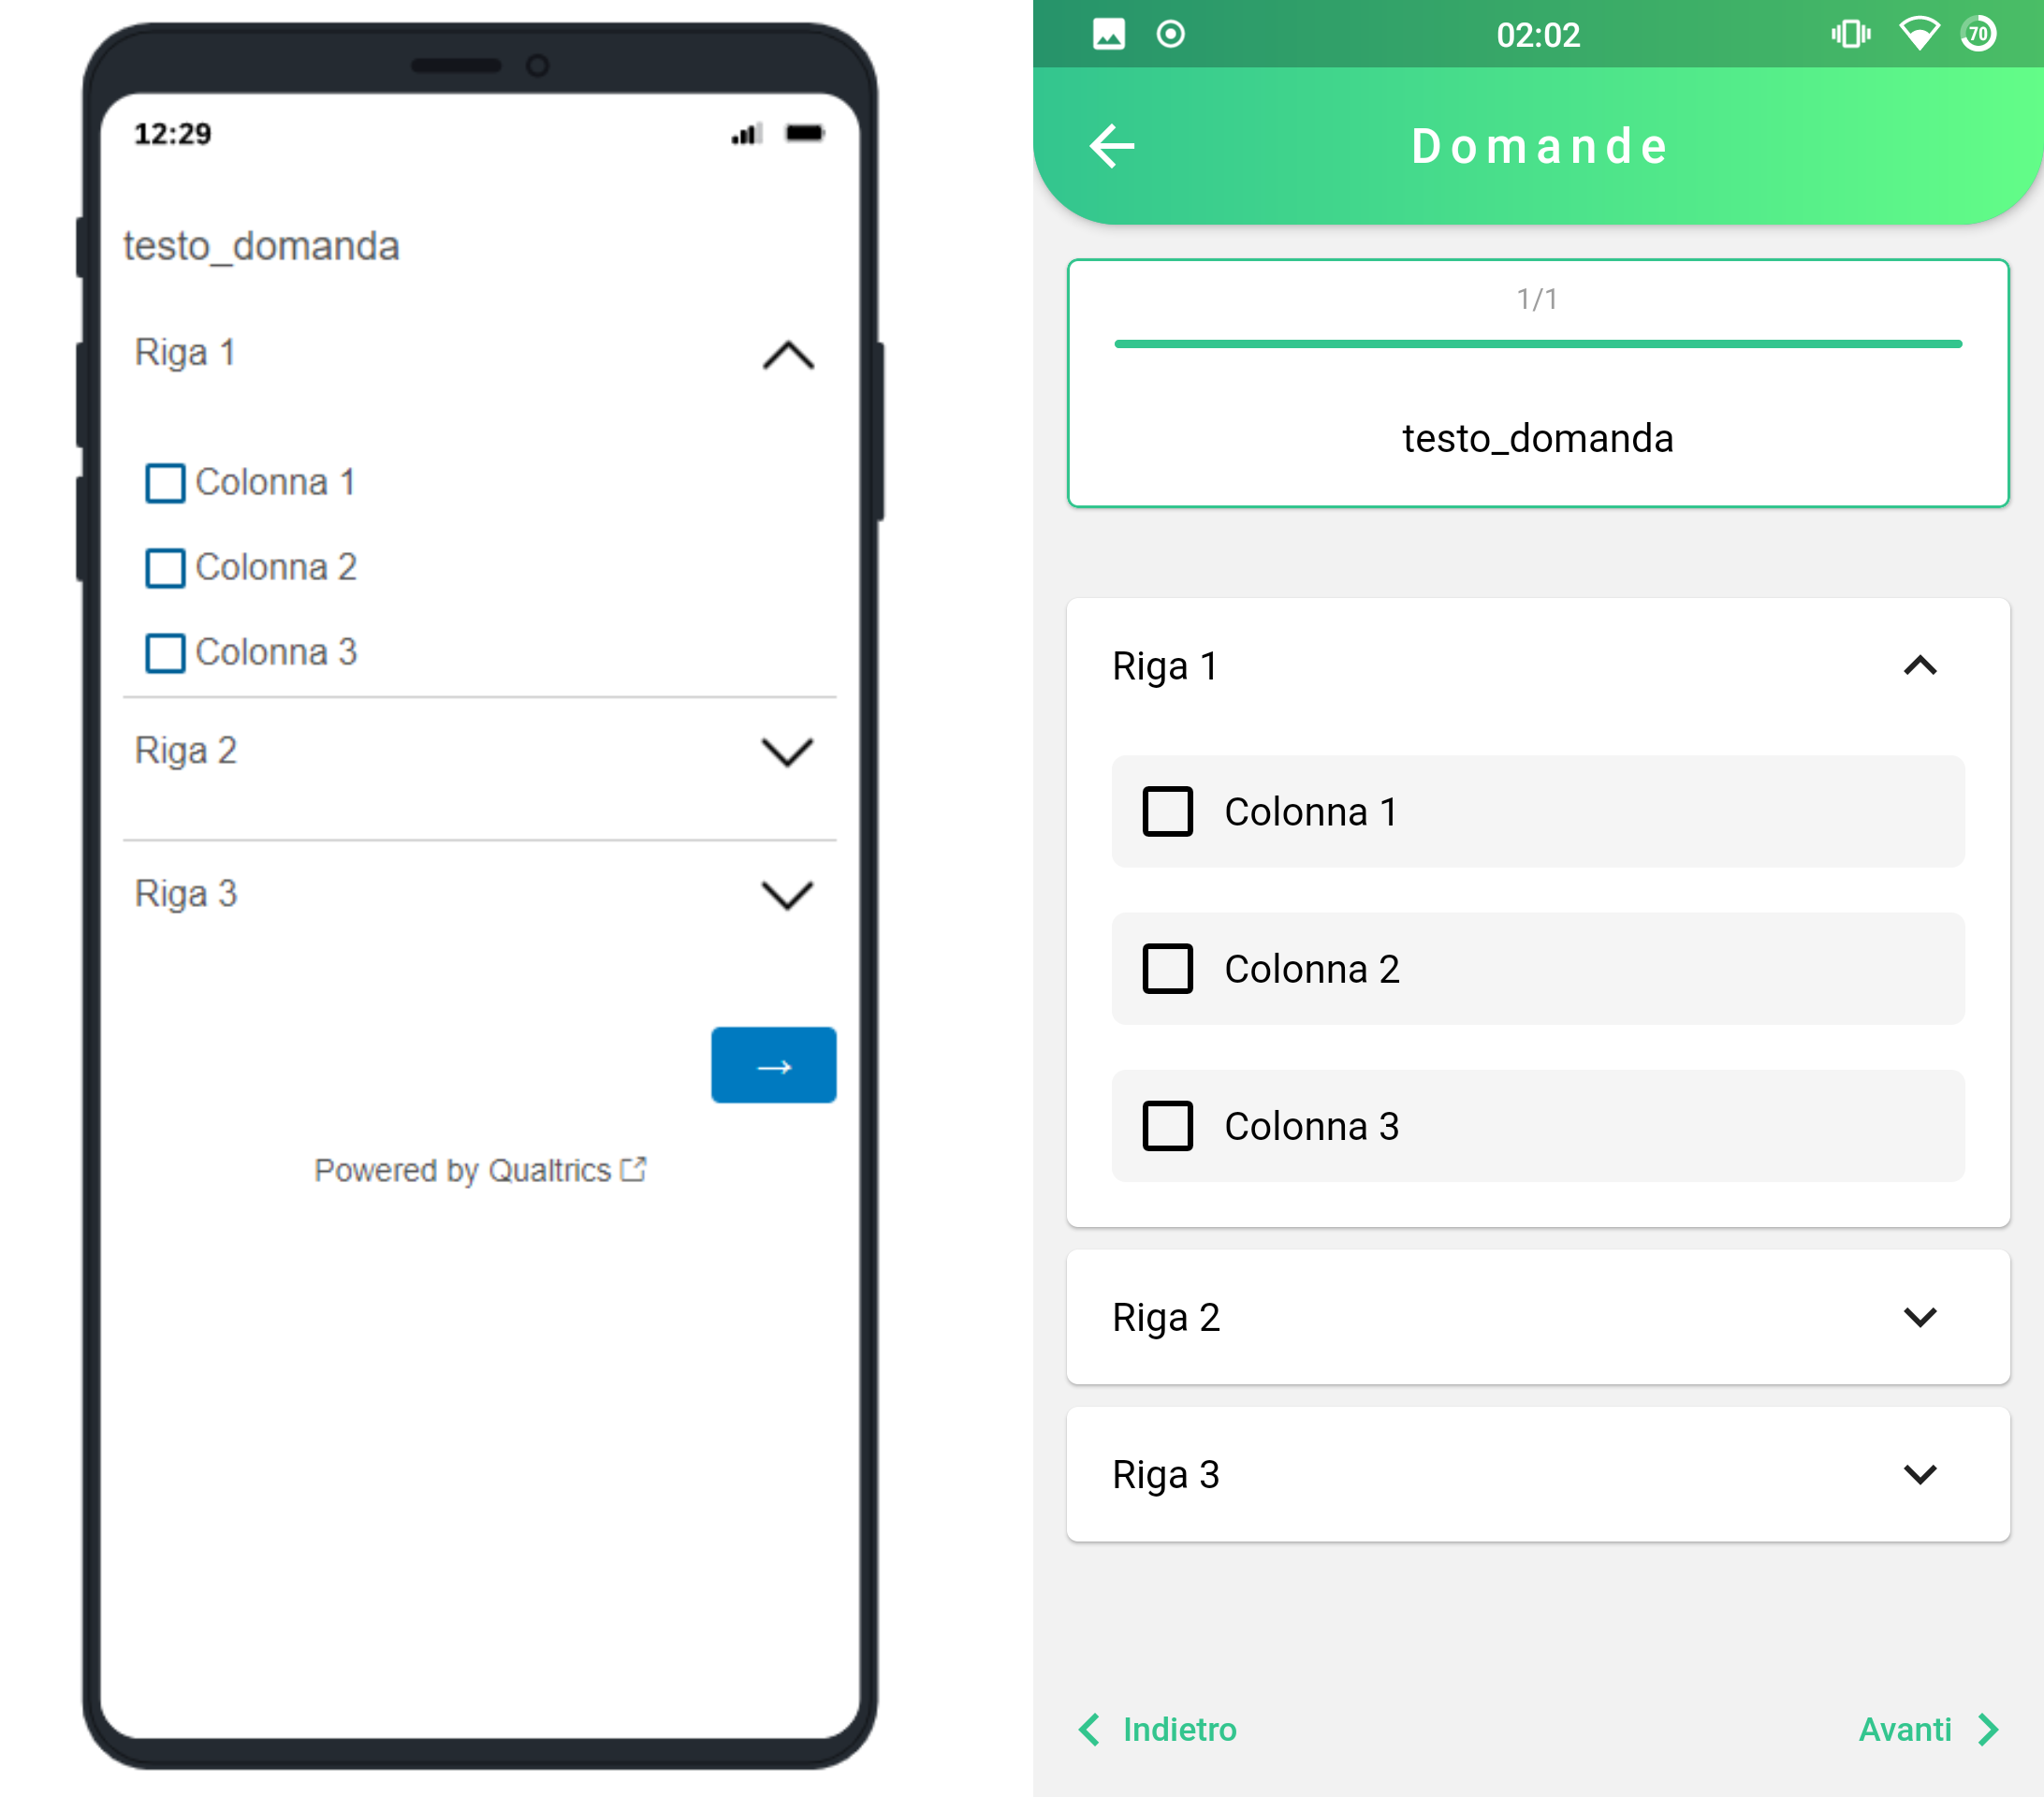
\includegraphics[width=0.7\textwidth]{img/matrix_likert}
\caption{Matrix Likert}
\label{fig:matrix_likert}
\end{figure}

\subsubsection{Matrix: "Selector": "Bipolar"}
Le matrici di tipo Bipolar permettono di selezionare una risposta che si avvicini di più ad una di due possibili scelte. Permettono dunque solo risposte singole. Il testo delle \texttt{Choice} tuttavia è "separato" in due parti utilizzando il carattere ':'. Se viene utilizzato tale carattere nel testo stesso delle scelte tuttavia questo viene preceduto da una coppia di caratteri di escape da Qualtrics. È stato dunque necessario identificare e trattare nel modo desiderato tale escaping nell'applicazione, operazione eseguita tramite delle espressioni regolari che, nel caso trovassero una espressione '\textbackslash\textbackslash:' rimuovessero i caratteri di escape e stampassero il ':', mentre nel caso trovassero un ':' senza escaping dividessero la stringa in due, in modo da avere parte destra e sinistra del testo della scelta. Possiamo osservare un esempio di questa domanda nella \autoref{fig:matrix_bipolar} dove possiamo anche osservare come la webview mobile di Qualtrics non sia ottimale e non sopporti nemmeno le label.

\paragraph{Response:}
Le risposte, essendo una matrice che accetta solo risposte singole, sono del tipo \texttt{\{"QuestionID\_ChoiceID": AnswerID\}}.

\begin{figure}[h!]
\centering
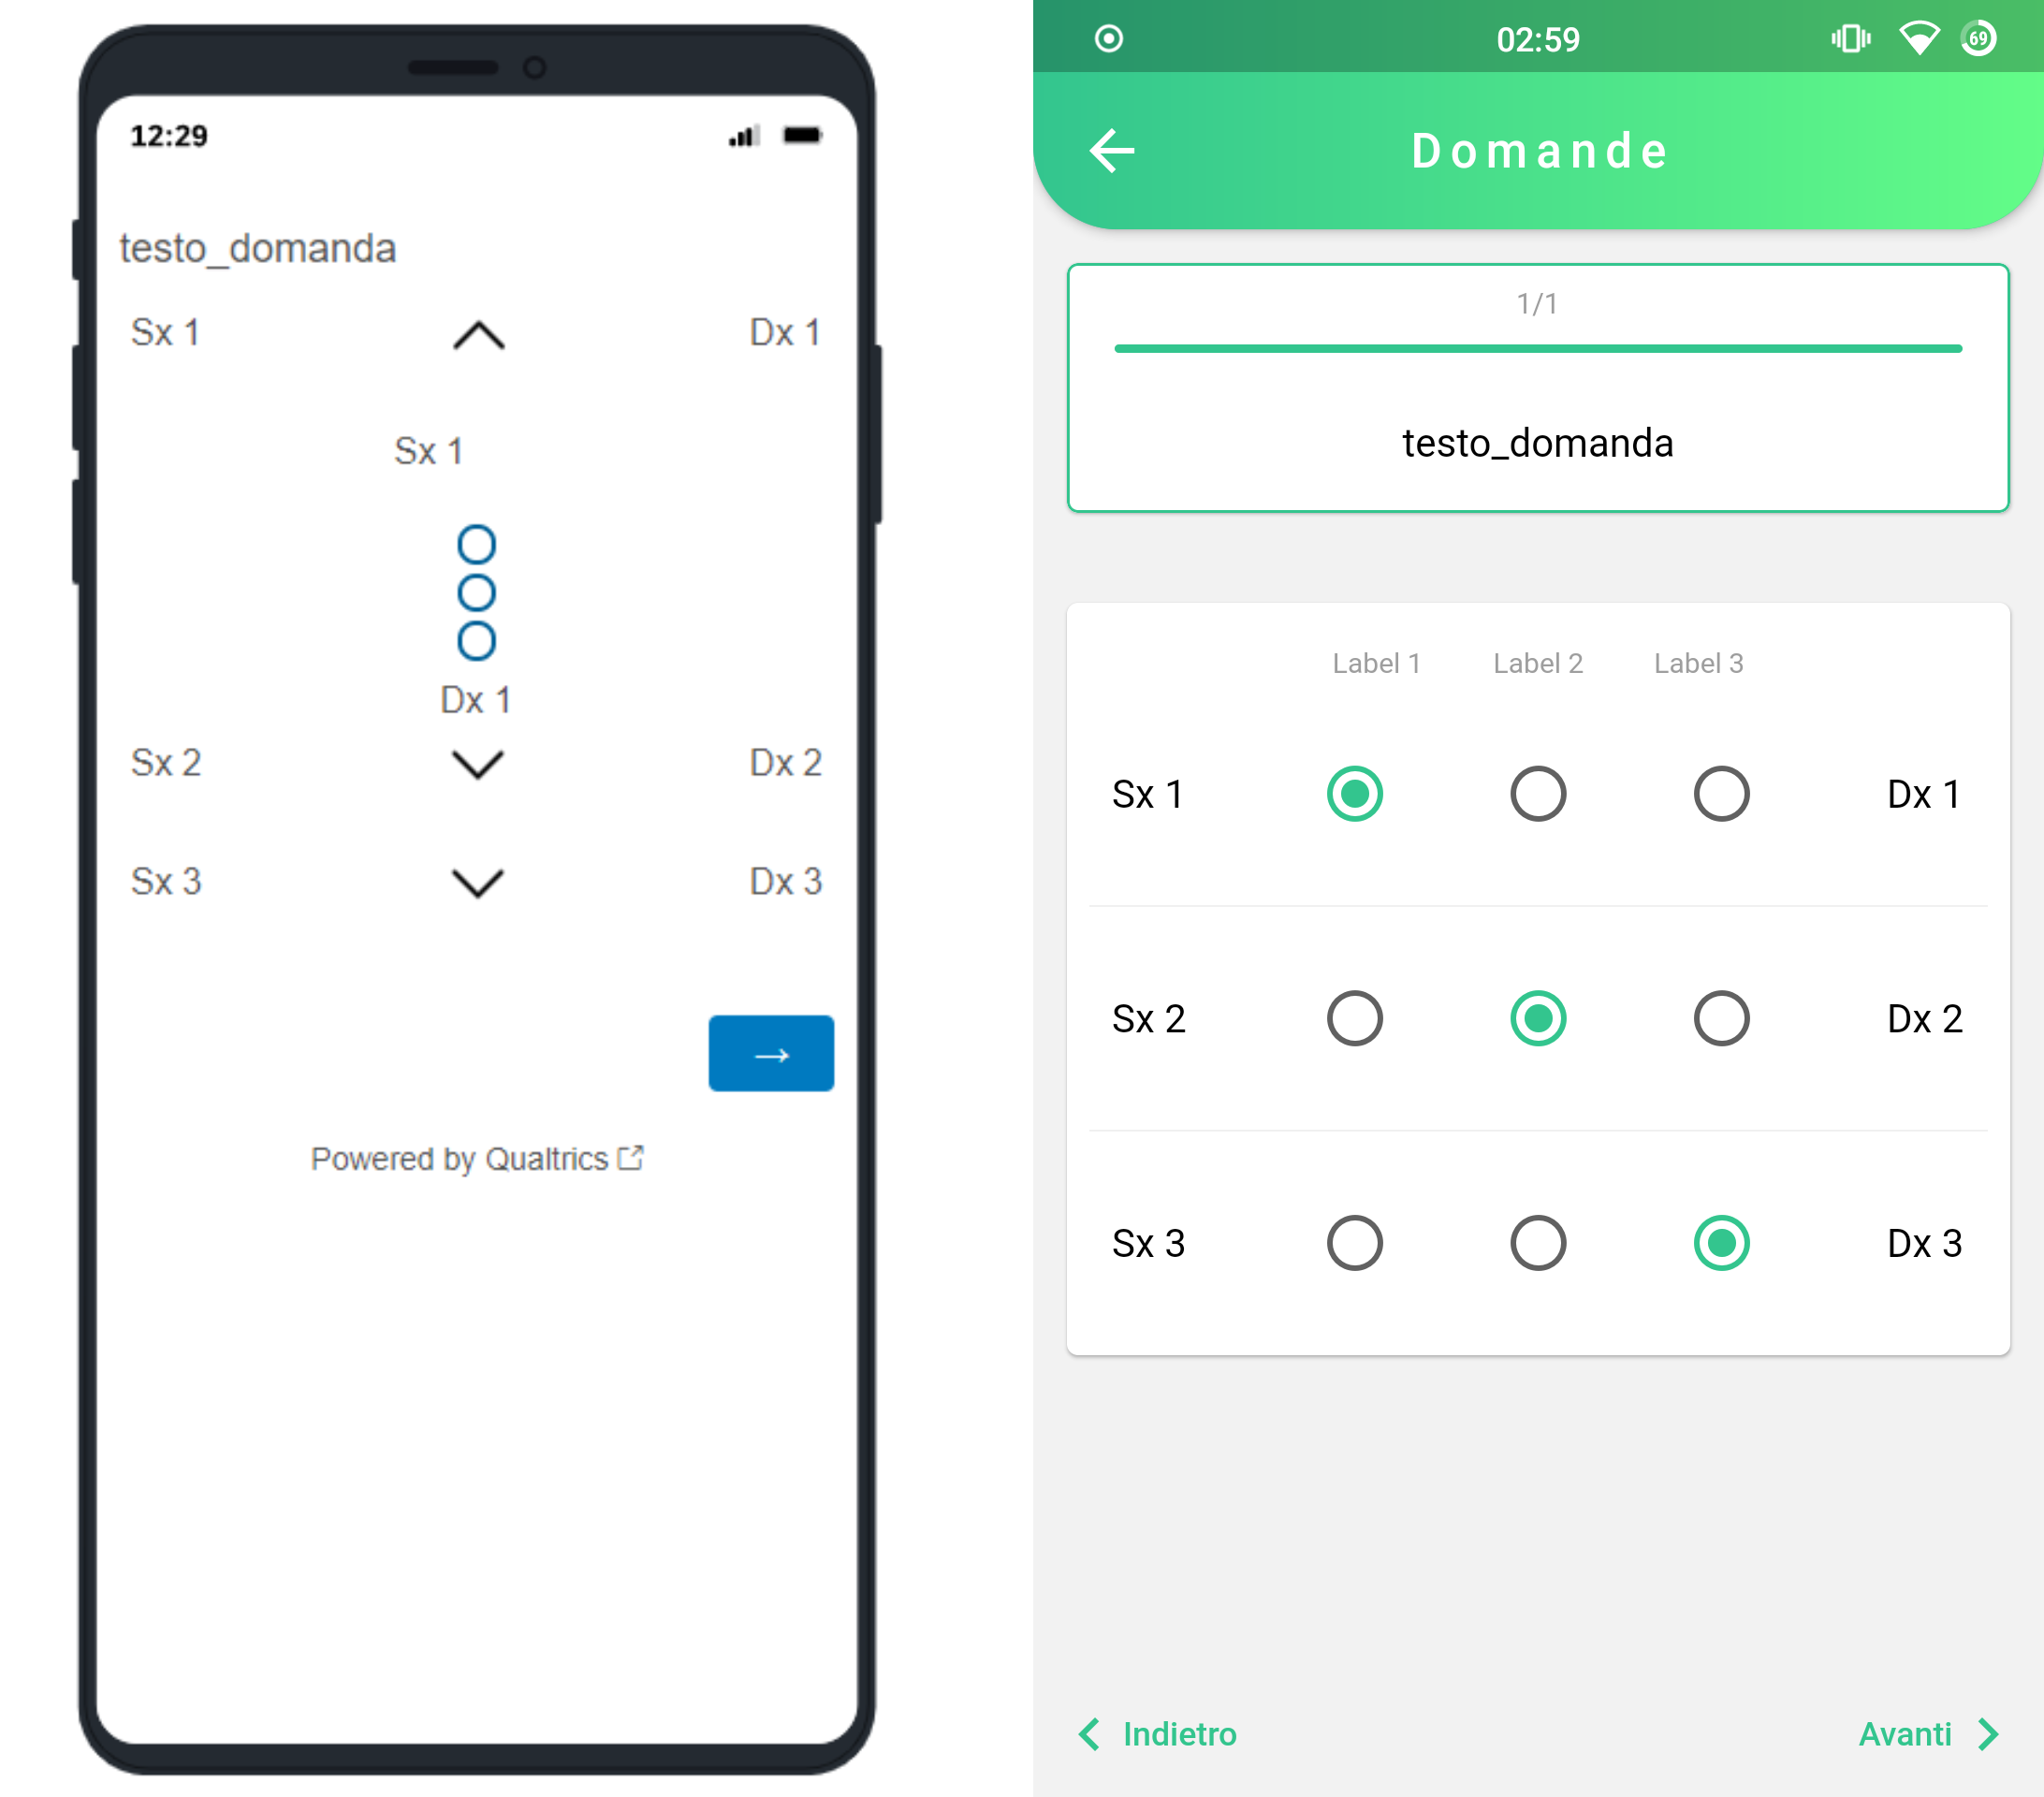
\includegraphics[width=0.7\textwidth]{img/matrix_bipolar}
\caption{Matrix Bipolar}
\label{fig:matrix_bipolar}
\end{figure}

\clearpage
\subsubsection{Matrix: "Selector": "MaxDiff"}
Un altro tipo di matrice che supporta solo risposte singole è il MaxDiff che è il sotto-tipo duale delle Bipolar: permette di scegliere solo tra due risposte \textit{(ad esempio Si/No)}. Non hanno il problema della divisione del testo delle opzioni dunque. Possiamo osservare un esempio di questo tipo di domanda nella \autoref{fig:matrix_maxdiff}.

\paragraph{Response:}
Anche in questo caso, essendo una domanda che accetta solo risposte singole, le risposte sono del tipo \texttt{\{"QuestionID\_ChoiceID": AnswerID\}}.

\begin{figure}[h!]
\centering
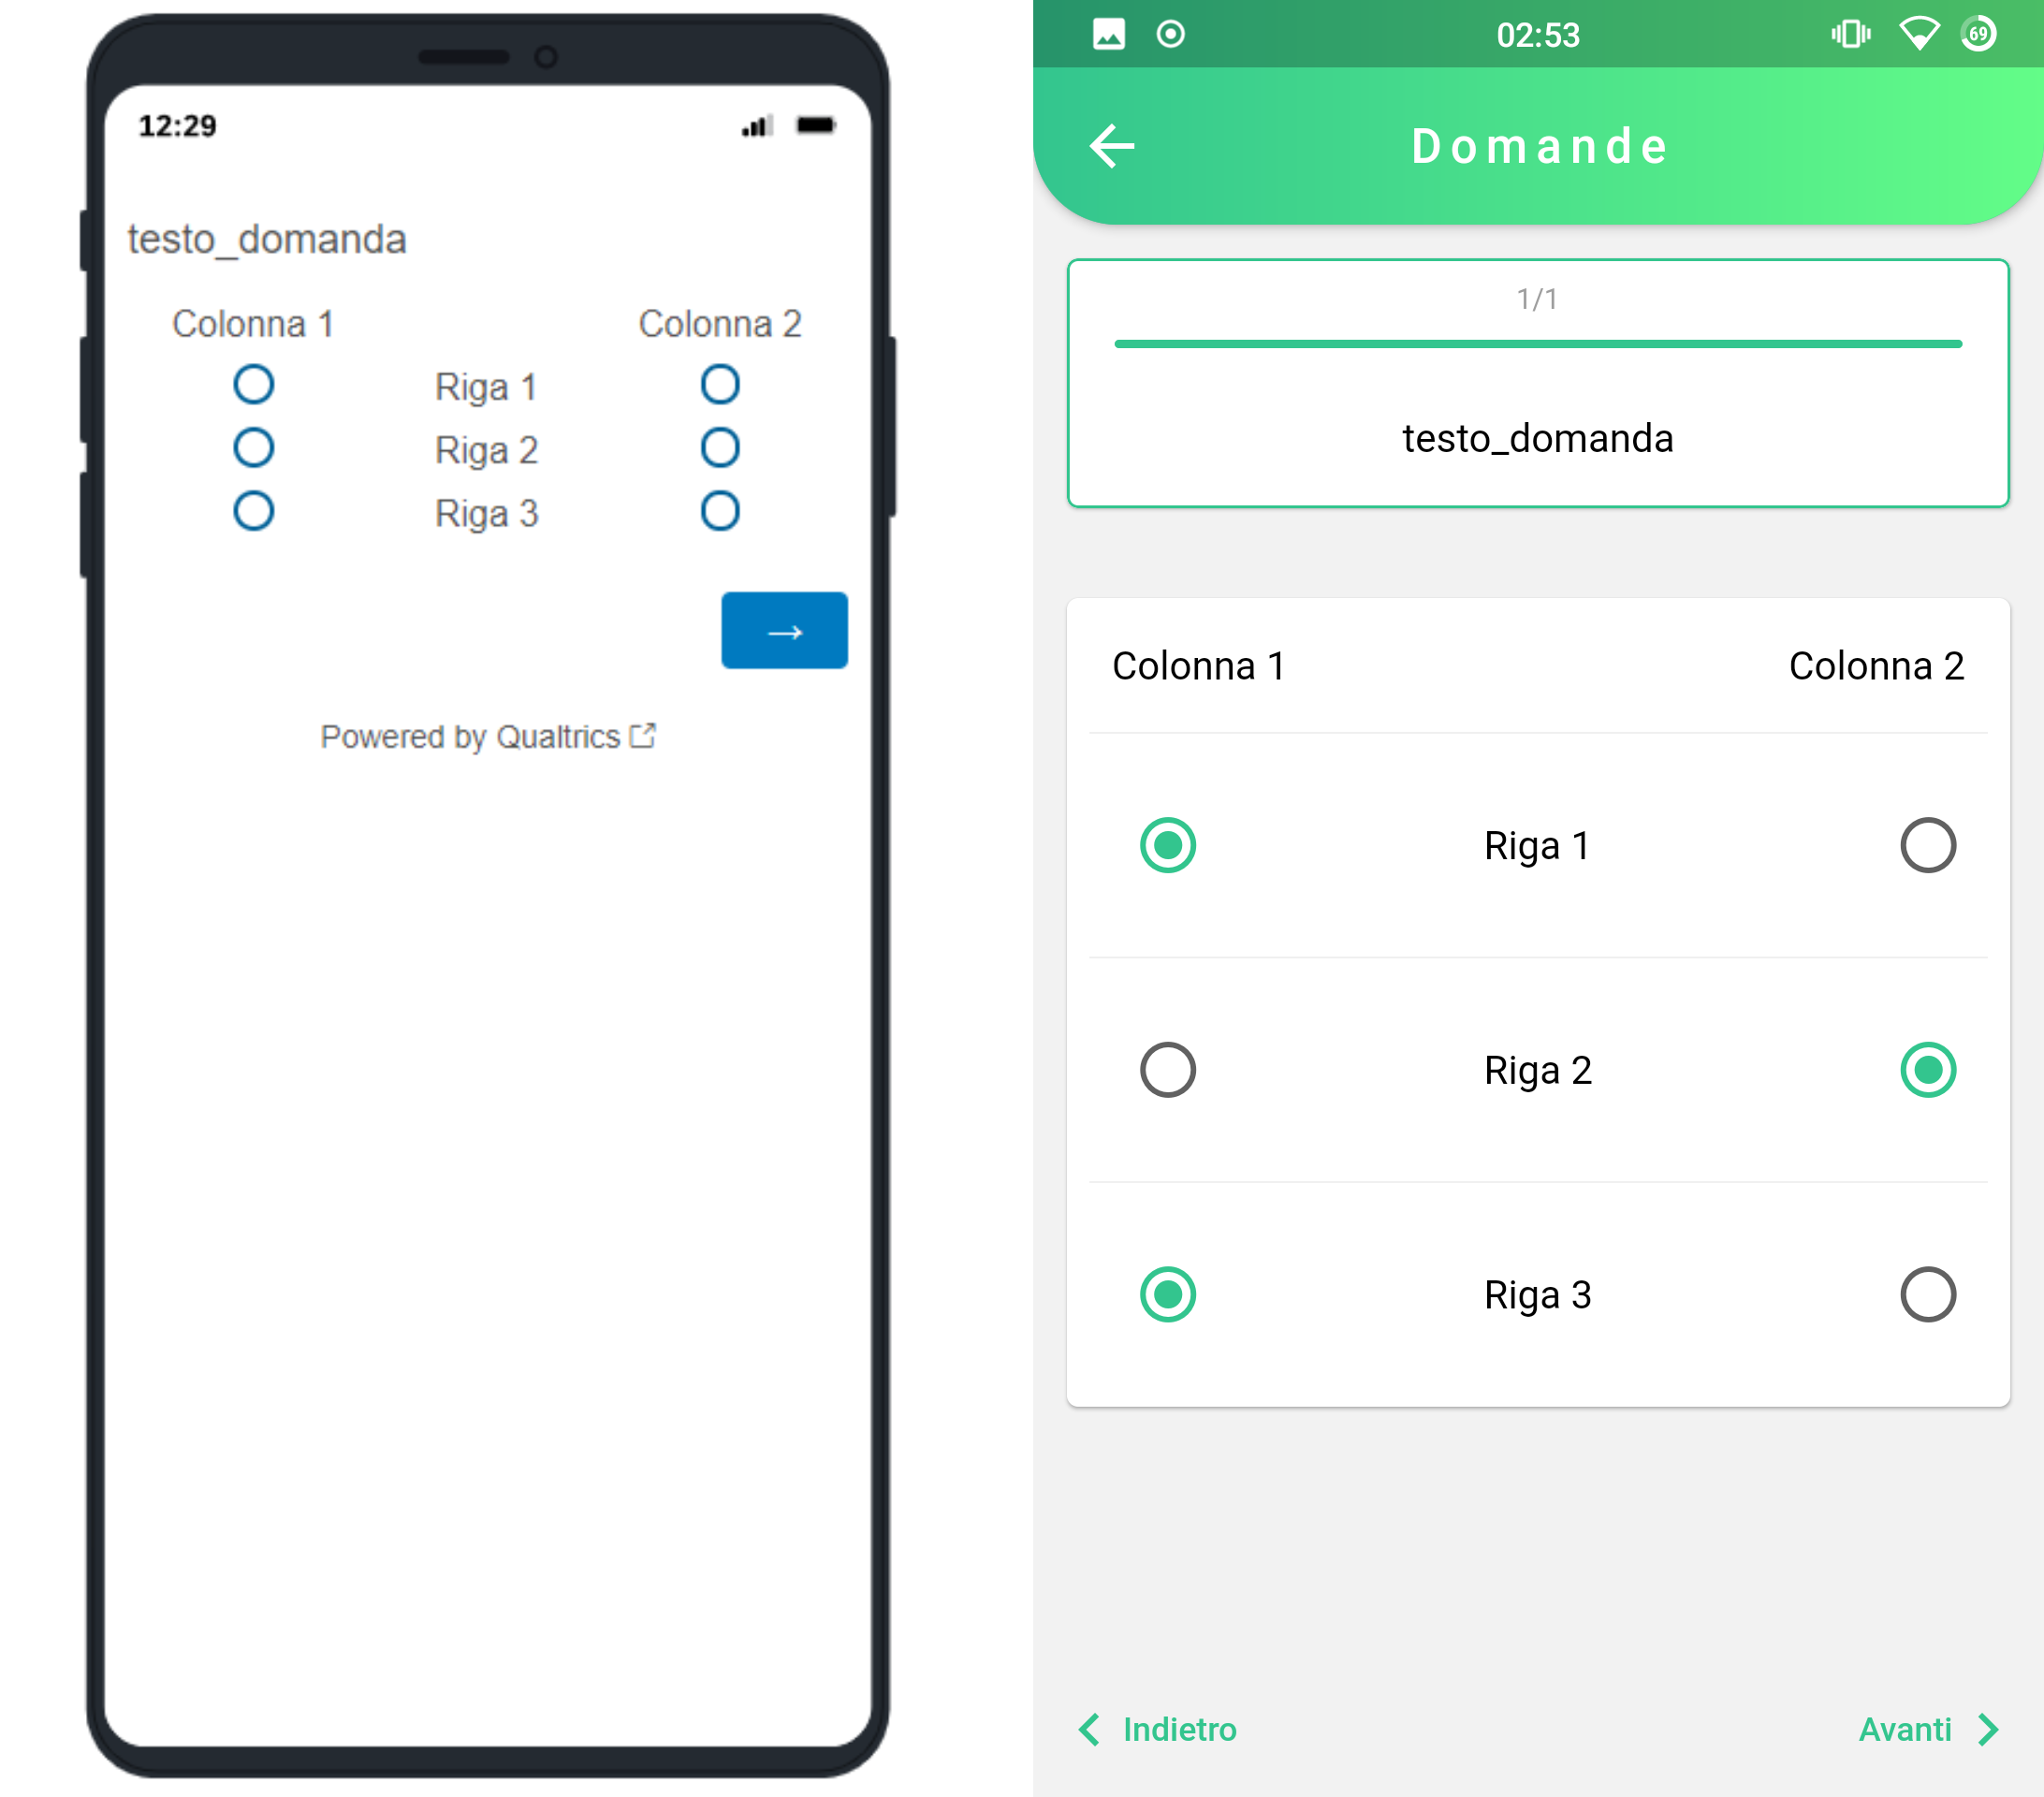
\includegraphics[width=0.7\textwidth]{img/matrix_maxdiff}
\caption{Matrix MaxDiff}
\label{fig:matrix_maxdiff}
\end{figure}

\clearpage
\subsubsection{Matrix: "Selector": "TextEntry"}
Una matrice simile alle Likert è la matrice Text Entry che, invece che avere delle risposte chiuse, permette di scrivere una risposta aperta per ogni sotto-domanda. Possiamo notare in \autoref{fig:matrix_te} come anche lo stile adottato richiama molto le matrici Likert, proprio per creare un design coerente in tutta l'applicazione.

\paragraph{Response:}
Le risposte di questo tipo di domande sono del tipo\\ \texttt{\{"QuestionID\_ChoiceID": "testo"\}}.\\Nel caso un'opzione prevedesse una text entry aggiuntiva, la risposta a tale text entry è del tipo \texttt{\{"QuestionID\_ChoiceID\_TEXT": "testo"\}}.

\begin{figure}[h!]
\centering
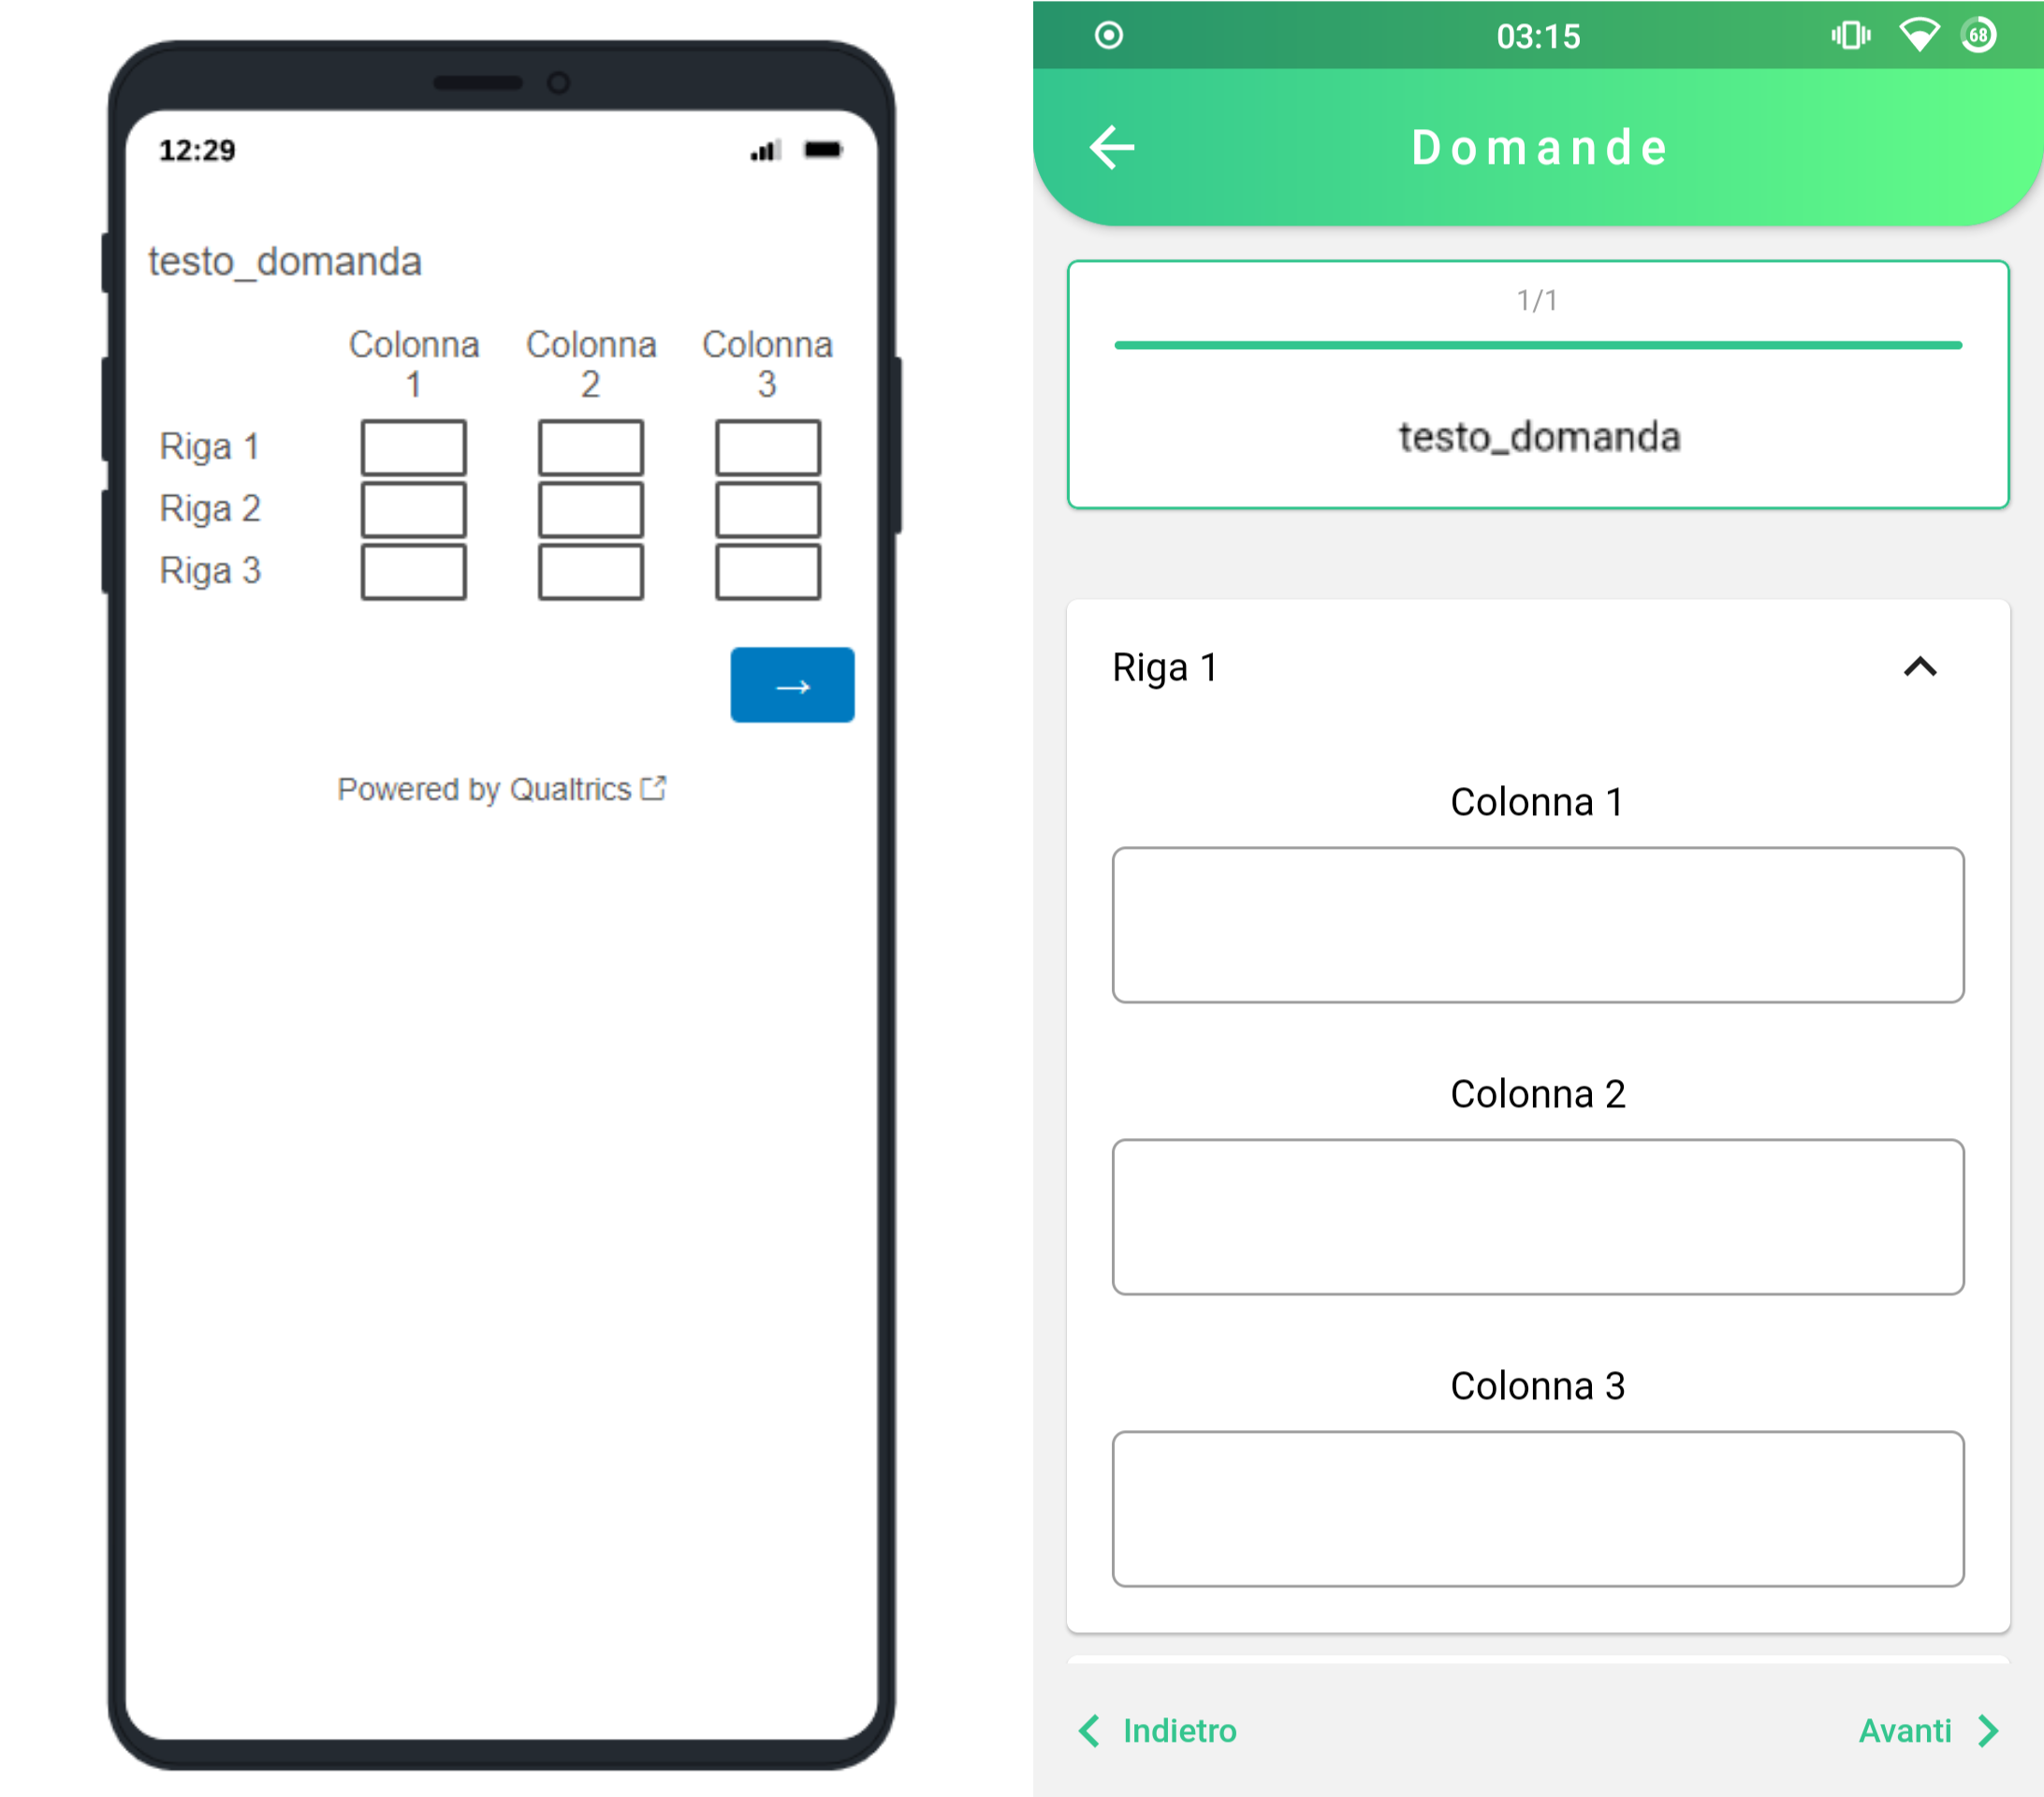
\includegraphics[width=0.7\textwidth]{img/matrix_te}
\caption{Matrix Text Entry}
\label{fig:matrix_te}
\end{figure}

\clearpage
\subsubsection{Matrix: "Selector": "RO"}
Anche le matrici di tipo Rank Order somigliano molto alle matrici Likert, ma hanno un campo di input in cui l'utente può inserire un numero: queste domande richiedono all'utente di definire un ordine tra le varie opzioni assegnando dei numeri interi ad ogni opzione. Possiamo notare nella \autoref{fig:matrix_ro} come lo stile adottato sia molto simile allo stile delle matrici Text Entry ma con un campo di input minore, essendo necessario meno spazio per inserire dei numeri.

\paragraph{Response:}
Le risposte di questo tipo di domande sono del tipo\\ \texttt{\{"QuestionID\_ChoiceID": numero\}}.\\Nel caso un'opzione prevedesse una text entry, la risposta a tale texte entry è del tipo \texttt{\{"QuestionID\_ChoiceID\_TEXT": "testo"\}}.

\begin{figure}[h!]
\centering
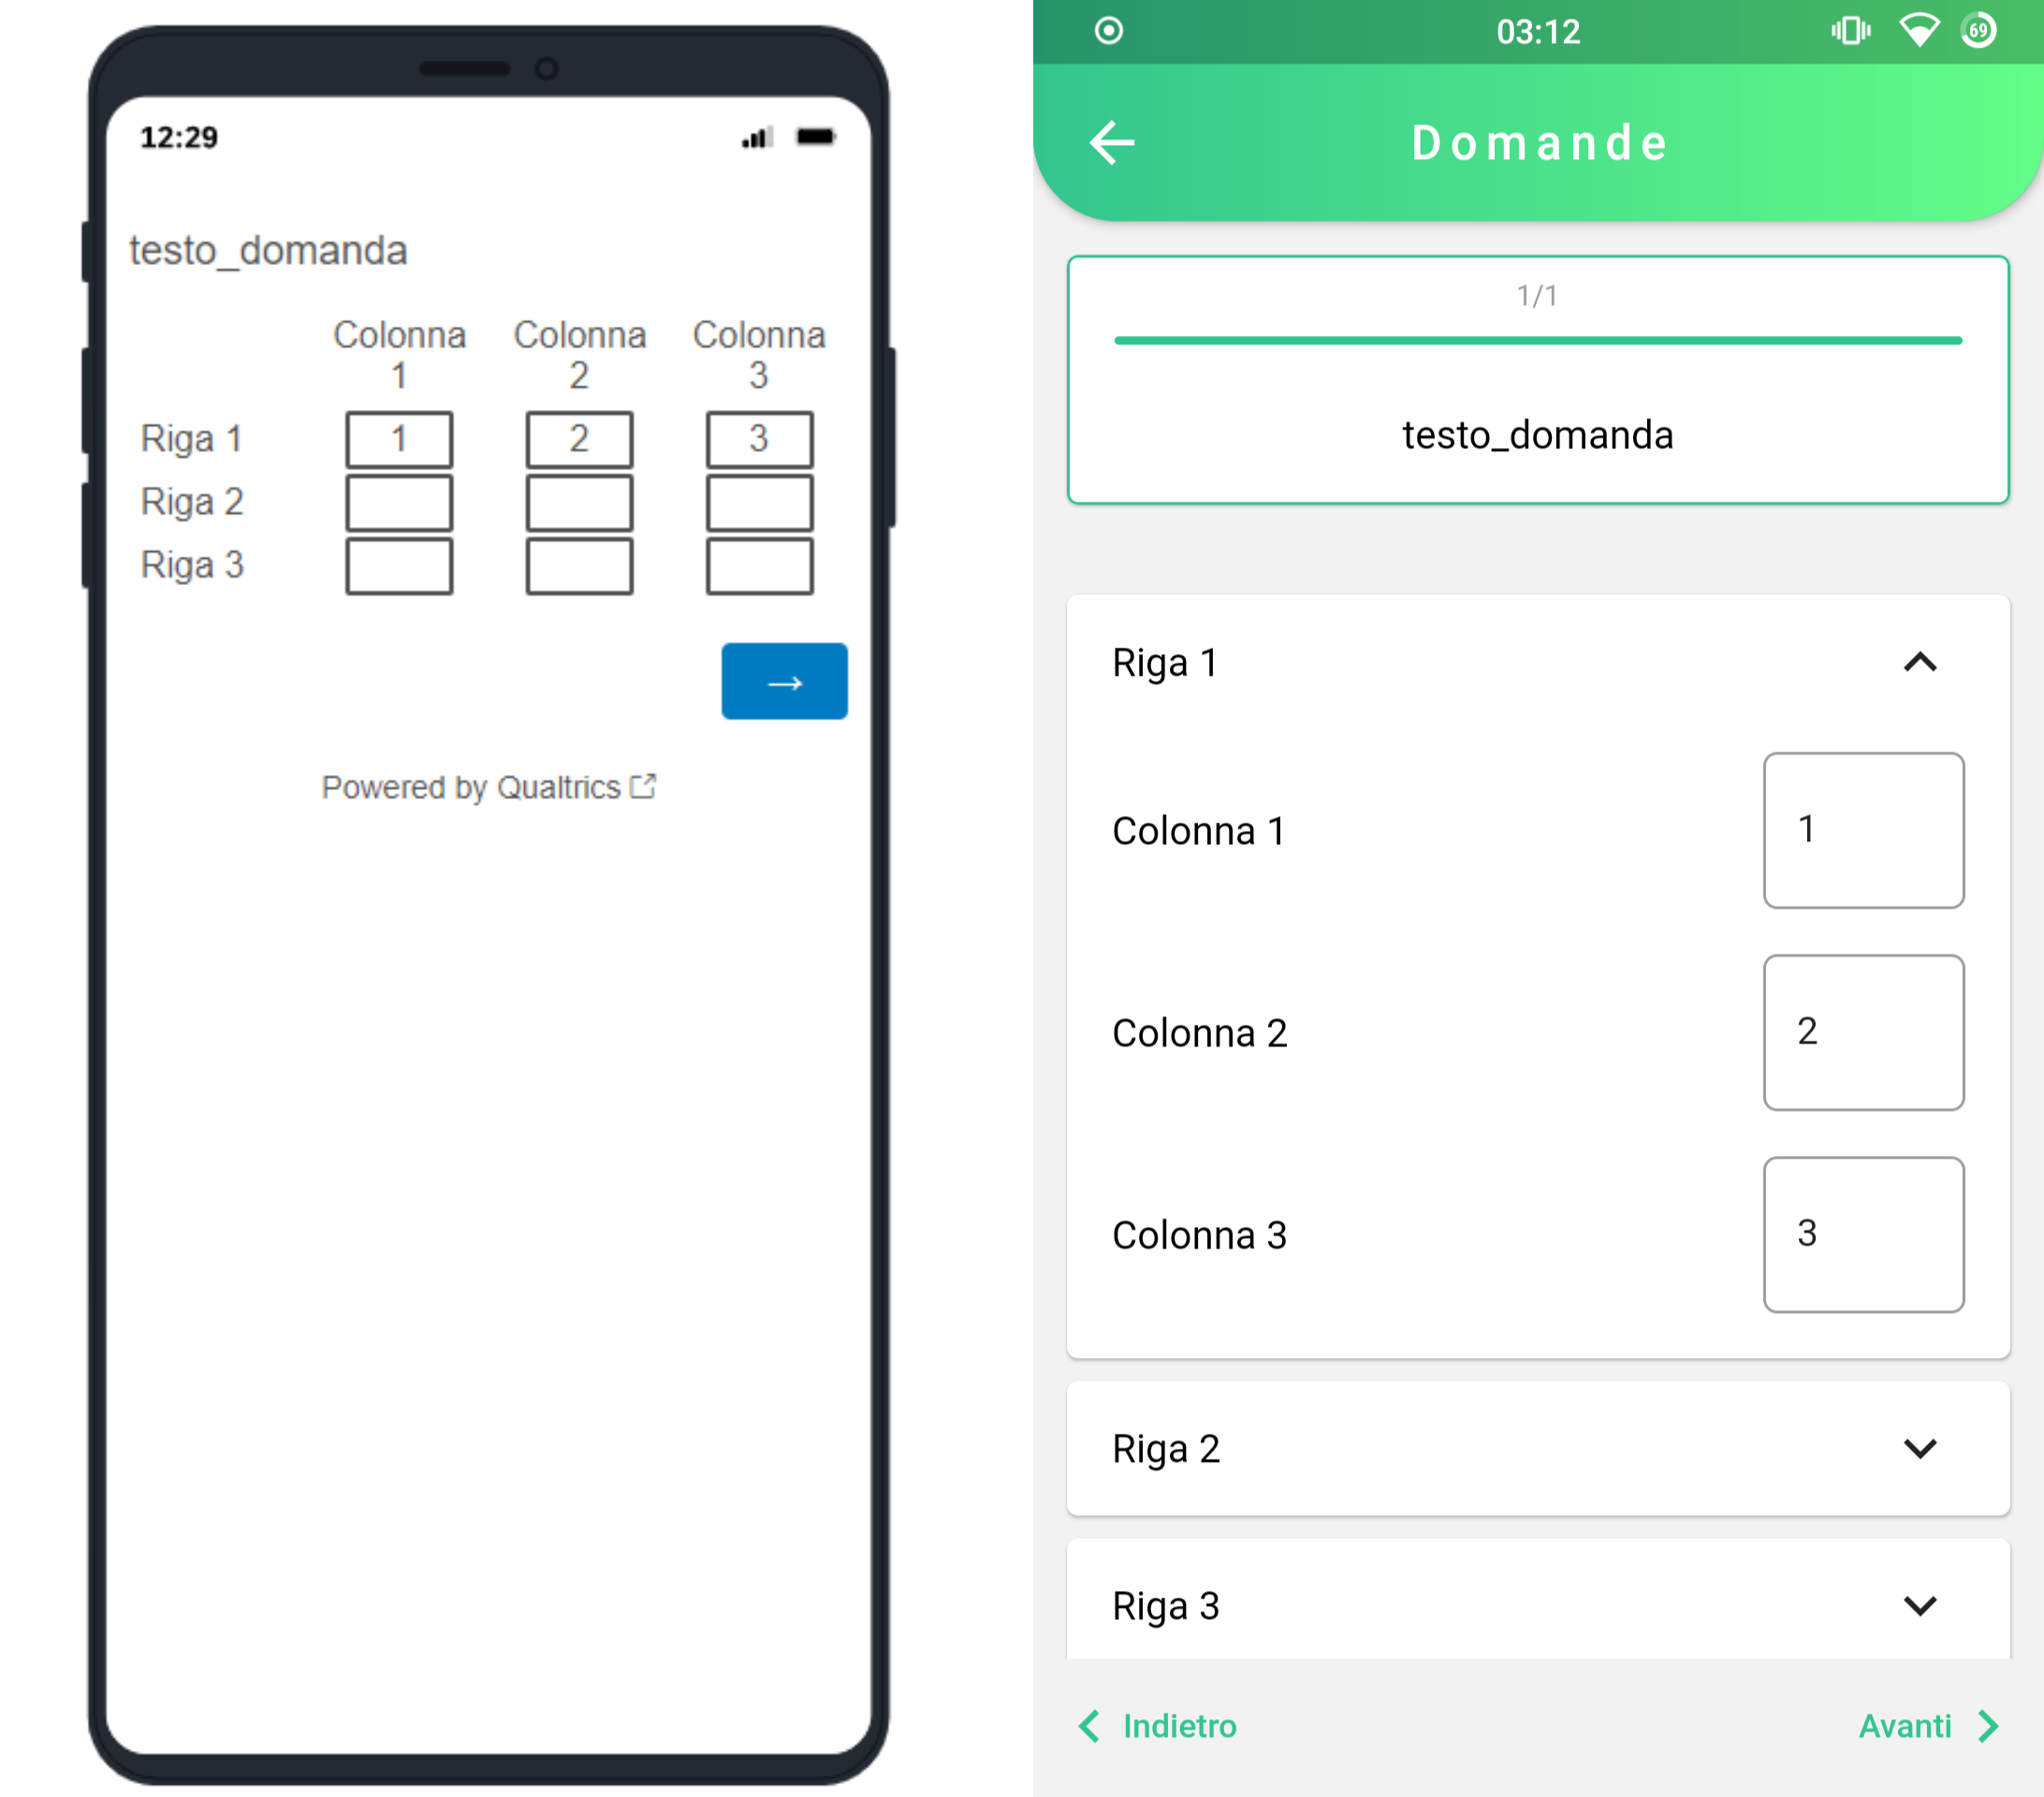
\includegraphics[width=0.7\textwidth]{img/matrix_ro}
\caption{Matrix Rank Order}
\label{fig:matrix_ro}
\end{figure}

\clearpage
\subsubsection{Matrix: "Selector": "CS"}
Anche questo ultimo tipo di matrici è simile alle Text Entry: permette di inserire dei numeri come le Rank Order ma che non hanno lo scopo di ordinare le risposte. Queste matrici riportano infine la somma di tutti i numeri inseriti nelle varie opzioni. È possibile osservare nella \autoref{fig:matrix_cs} come lo stile adottato sia molto simile alle matrici Rank Order, visto che accettano lo stesso tipo di input.

\paragraph{Response:}
Le risposte di questo tipo di domande sono del tipo\\ \texttt{\{"QuestionID\_ChoiceID": numero\}}.\\Nel caso un'opzione prevedesse una text entry, la risposta a tale texte entry è del tipo \texttt{\{"QuestionID\_ChoiceID\_TEXT": "testo"\}}.

\begin{figure}[h!]
\centering
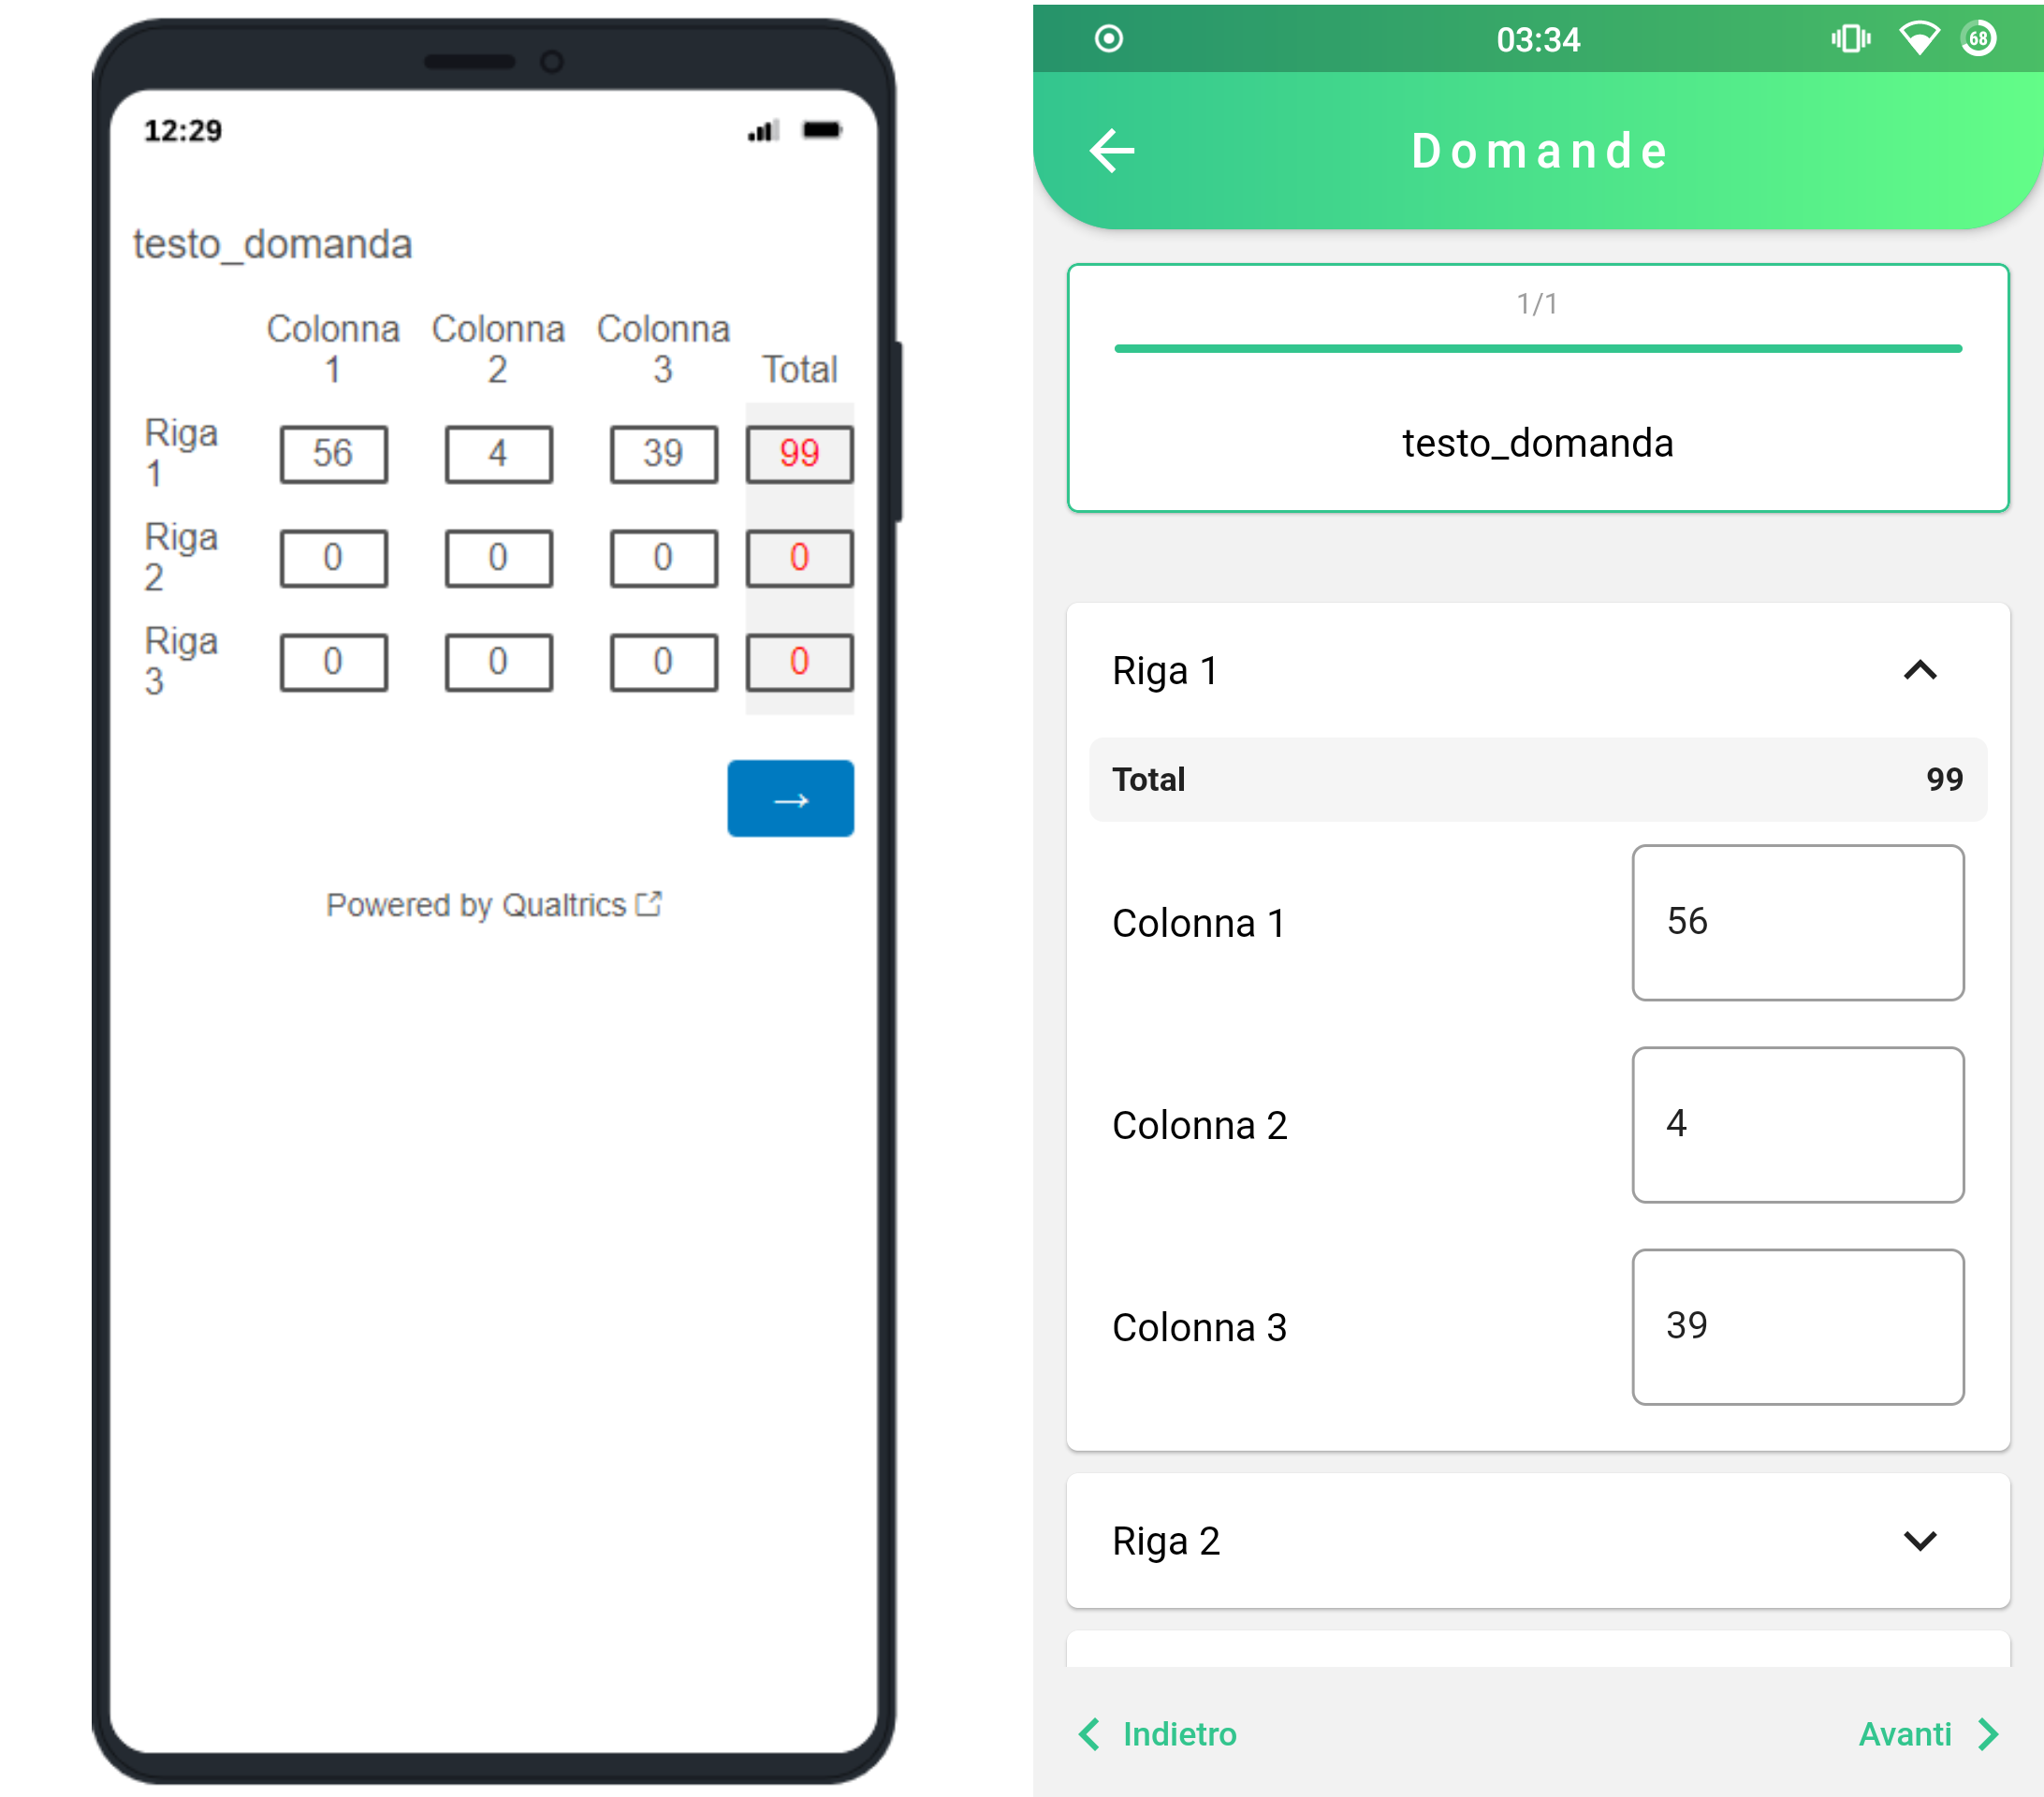
\includegraphics[width=0.7\textwidth]{img/matrix_cs}
\caption{Matrix Costant Sum}
\label{fig:matrix_cs}
\end{figure}

\clearpage
\subsection{Side By Side - "QuestionType": "SBS"}
Il tipo di domanda Side By Side è un'evoluzione delle matrici precedenti: questo tipo di domanda permette di avere domande completamente diverse in un'unica tabella \textit{(quindi che abbiano anche risposte di diverso tipo, oltre che diverse come nelle matrici profile)}. In particolare, i tipi di risposta possono essere Single Answer, SA con menù a tendina, Multiple Answers e Text Entry. Inoltre, come possiamo vedere nella \autoref{fig:sbs}, a differenza delle matrici semplici è possibile anche definire un numero di risposte variabile per ogni sotto-domanda. Possiamo osservare la struttura di questo tipo di domande nel \autoref{json:sbs} ed è subito notabile una particolarità: nell'oggetto \texttt{AdditionalQuestions} vengono salvati effettivamente degli oggetti che descrivono delle matrici come visto precedentemente, ognuna con le proprie \texttt{Answers} \textit{(le \texttt{Choices} sono le stesse dell'oggetto SBS stesso)} e soprattutto ognuna col proprio \texttt{QuestionID}, parametro molto importante per costruire poi le risposte.

\subsubsection{Media}
Come per le matrici, anche le Side By Side supportano immagini su \texttt{Choices} e \texttt{Answers} e text entry aggiuntive sulle \texttt{Choices}.

\subsubsection{Response}
Avendo la domanda più domande interne indipendenti, le risposte sono separate e sono identificate da \texttt{QuestionID\#SubQuestionID\_ChoiceID} \textit{(il SubQuestionID è quello riportarto nel campo QuestionID delle sotto-domande nel campo AdditionalQuestions)}. Le risposte sono dunque del tipo\\ \texttt{\{"QuestionID\#SubQuestionID\_ChoiceID": AnswerID\}} per una risposta singola, \texttt{\{"QuestionID\#SubQuestionID\_ChoiceID": ["AnswerID\_1", "AnswerID\_2"]\}}\\ per risposte multiple e \texttt{\{"QuestionID\#SubQuestionID\_ChoiceID": "testo"\}} nel caso di text entry. \\
Nel caso fossero presenti text entry addizionali sulle \texttt{Choices}, la risposta a tali text entry è del tipo \texttt{\{"QuestionID\#SubQuestionID\_ChoiceID\_TEXT": "testo"\}}.

\newpage
\begin{json}
\usemintedstyle[JSON]{trac}
\begin{minted}[]{JSON}
{
    "QuestionText": "testo_domanda",
    "QuestionID": "QID257",
    "QuestionType": "SBS",
    "Choices": {},
    "AdditionalQuestions": {
        "1": {
            "Choices": {}
            "Answers": {},
            "QuestionText": "Colonna 1",
            "QuestionType": "Matrix",
            "Selector": "Likert",
            "SubSelector": "MultipleAnswer",
            "QuestionID": "QID257#1",
        },
    },
}
\end{minted}
\caption{Oggetto domanda Side By Side}
\label{json:sbs}
\end{json}

\begin{figure}[h!]
\centering
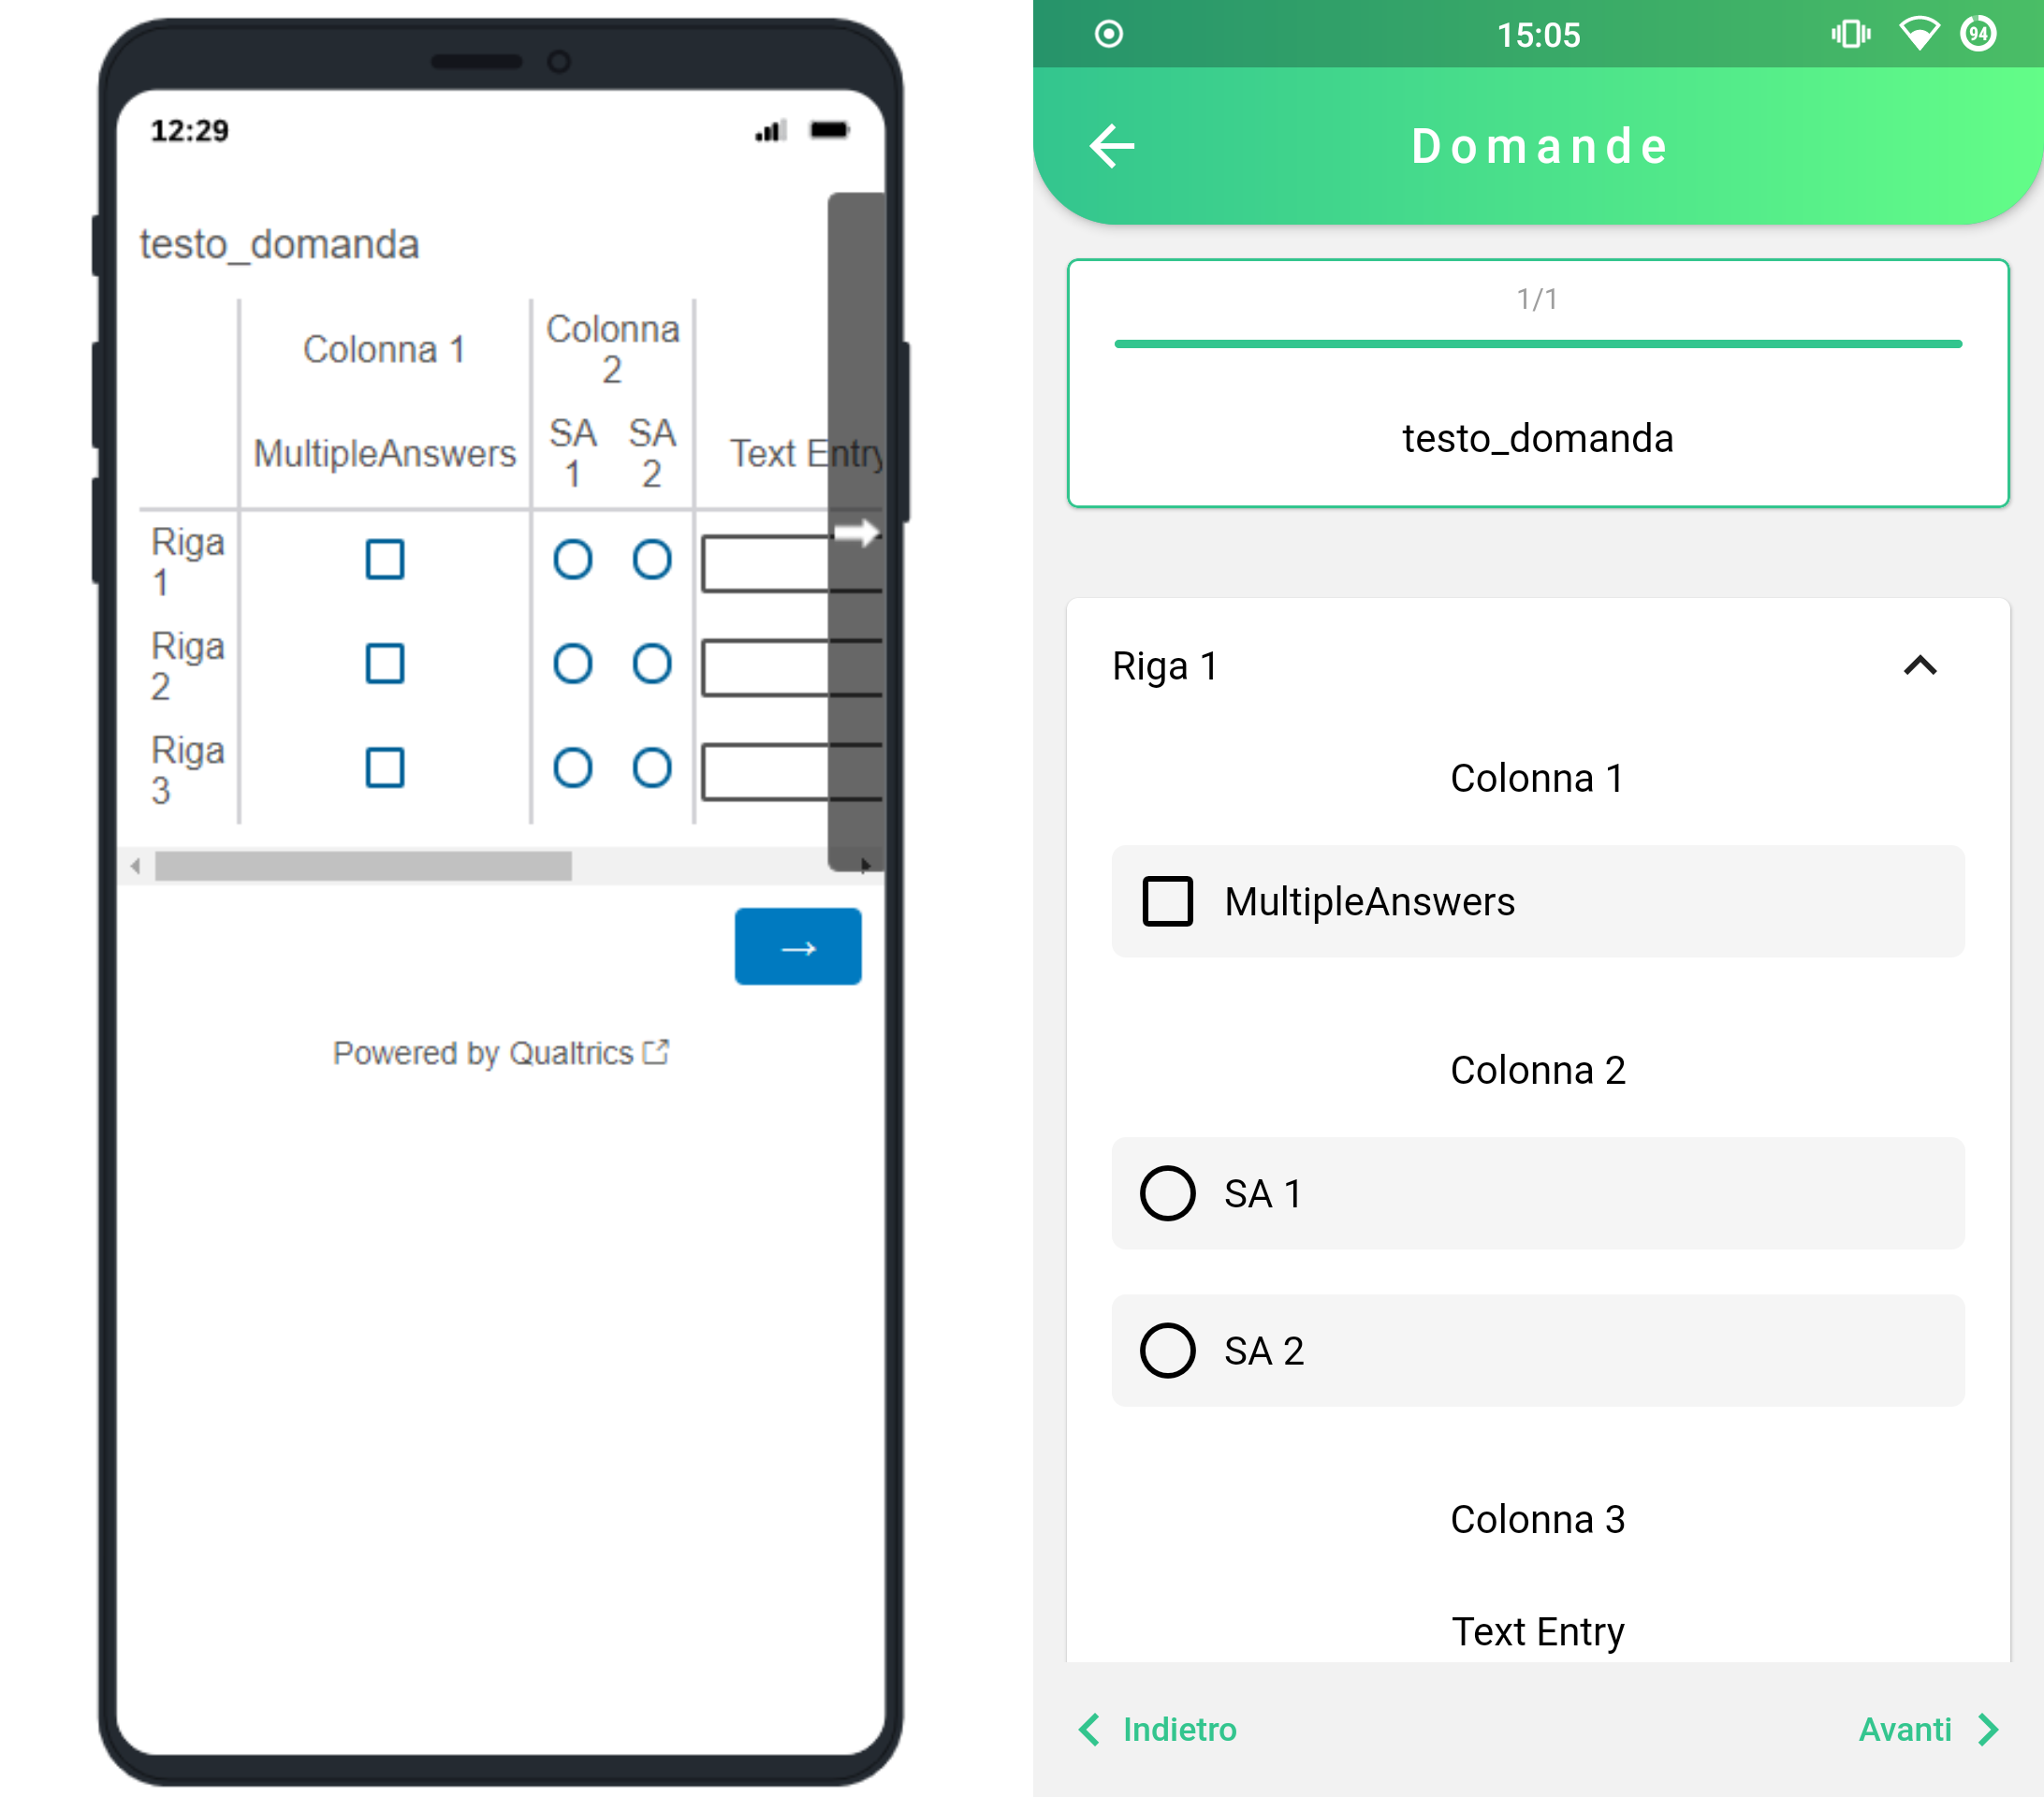
\includegraphics[width=0.66\textwidth]{img/sbs}
\caption{Side By Side}
\label{fig:sbs}
\end{figure}

\clearpage
\subsection{Slider - "QuestionType": "Slider"}
Un tipo di domanda molto utile messo a disposizione da Qualtrics è lo Slider, ovvero una domanda la cui risposta è esprimibile attraverso dei cursori interattivi, utile ad esprimere ad esempio livelli di preferenza o di intensità. Possiamo osservare la struttura di queste domande nel \autoref{json:slider}, in particolare possiamo osservare che una domanda di questo tipo può avere diversi slider, identificati dalle \texttt{Choices} e che, se impostato in modo che assuma solo determinati valori, questi sono presenti nel campo \texttt{Answers}. Di particolare interesse è il campo \texttt{Configuration} che permette di impostare alcuni parametri dello slider come potrebbero essere i valori minimi e massimi, determinati dai campi \texttt{CSSliderMin} e \texttt{CSSliderMax}. Se inoltre l'opzione \texttt{SnapToGrid} è attiva, lo slider assumerà solo i valori delle \texttt{GridLines} (quindi assumerà solo multipli di \texttt{CSSliderMax} / \texttt{GridLines}). Tramite la configurazione possiamo definire anche quali valori iniziali dovrà assumere ciascun slider, contenuti nel campo \texttt{SliderStartPositions}.
Per lo sviluppo di questo widget è stato utilizzato come base lo slider generale messo a disposizione da Flutter modificato in termini di aspetto e di funzionalità per supportare i valori iniziali e lo snap to grid. Possiamo osservare anche come sono visibili le grid lines all'interno dello slider stesso nella \autoref{fig:slider}.

\subsubsection{Media}
Anche in questo caso è possibile associare ad ogni \texttt{Choice} \textit{(quindi ad ogni slider in questo caso)} un'immagine e una text entry aggiuntiva.

\subsubsection{Response}
Le risposte a questo tipo di domande sono del tipo \texttt{\{"QuestionID\_ChoiceID": numero\}}, dove numero è il valore intero assunto dallo slider. Nel caso ci fosse una text entry aggiuntiva, la risposta sarà del tipo \texttt{\{"QuestionID\_ChoiceID\_TEXT": "testo"\}}.

\newpage
\begin{json}
\usemintedstyle[JSON]{trac}
\begin{minted}[]{JSON}
{
    "QuestionText": "testo_domanda",
    "QuestionID": "QID257",
    "QuestionType": "Slider",
    "Configuration": {
        "CSSliderMin": 0,
        "CSSliderMax": 100,
        "GridLines": 10,
        "SnapToGrid": true,
        "SliderStartPositions": {
            "1": 0,
            "2": 0.5
        }
    },
    "Choices": {
        "1": {
            "Display": "Slider 1"
        },
        "2": {
            "Display": "Slider 2"
        }
    },
    "ChoiceOrder": [],
    "Labels": {
        "1": {
            "Display": "Label 1"
        },
    },
    "Answers": {
        "1": {
            "Display": 0
        },
        "11": {
            "Display": 100
        }
    },
}
\end{minted}
\caption{Oggetto domanda Slider}
\label{json:slider}
\end{json}

\begin{figure}[ht!]
\centering
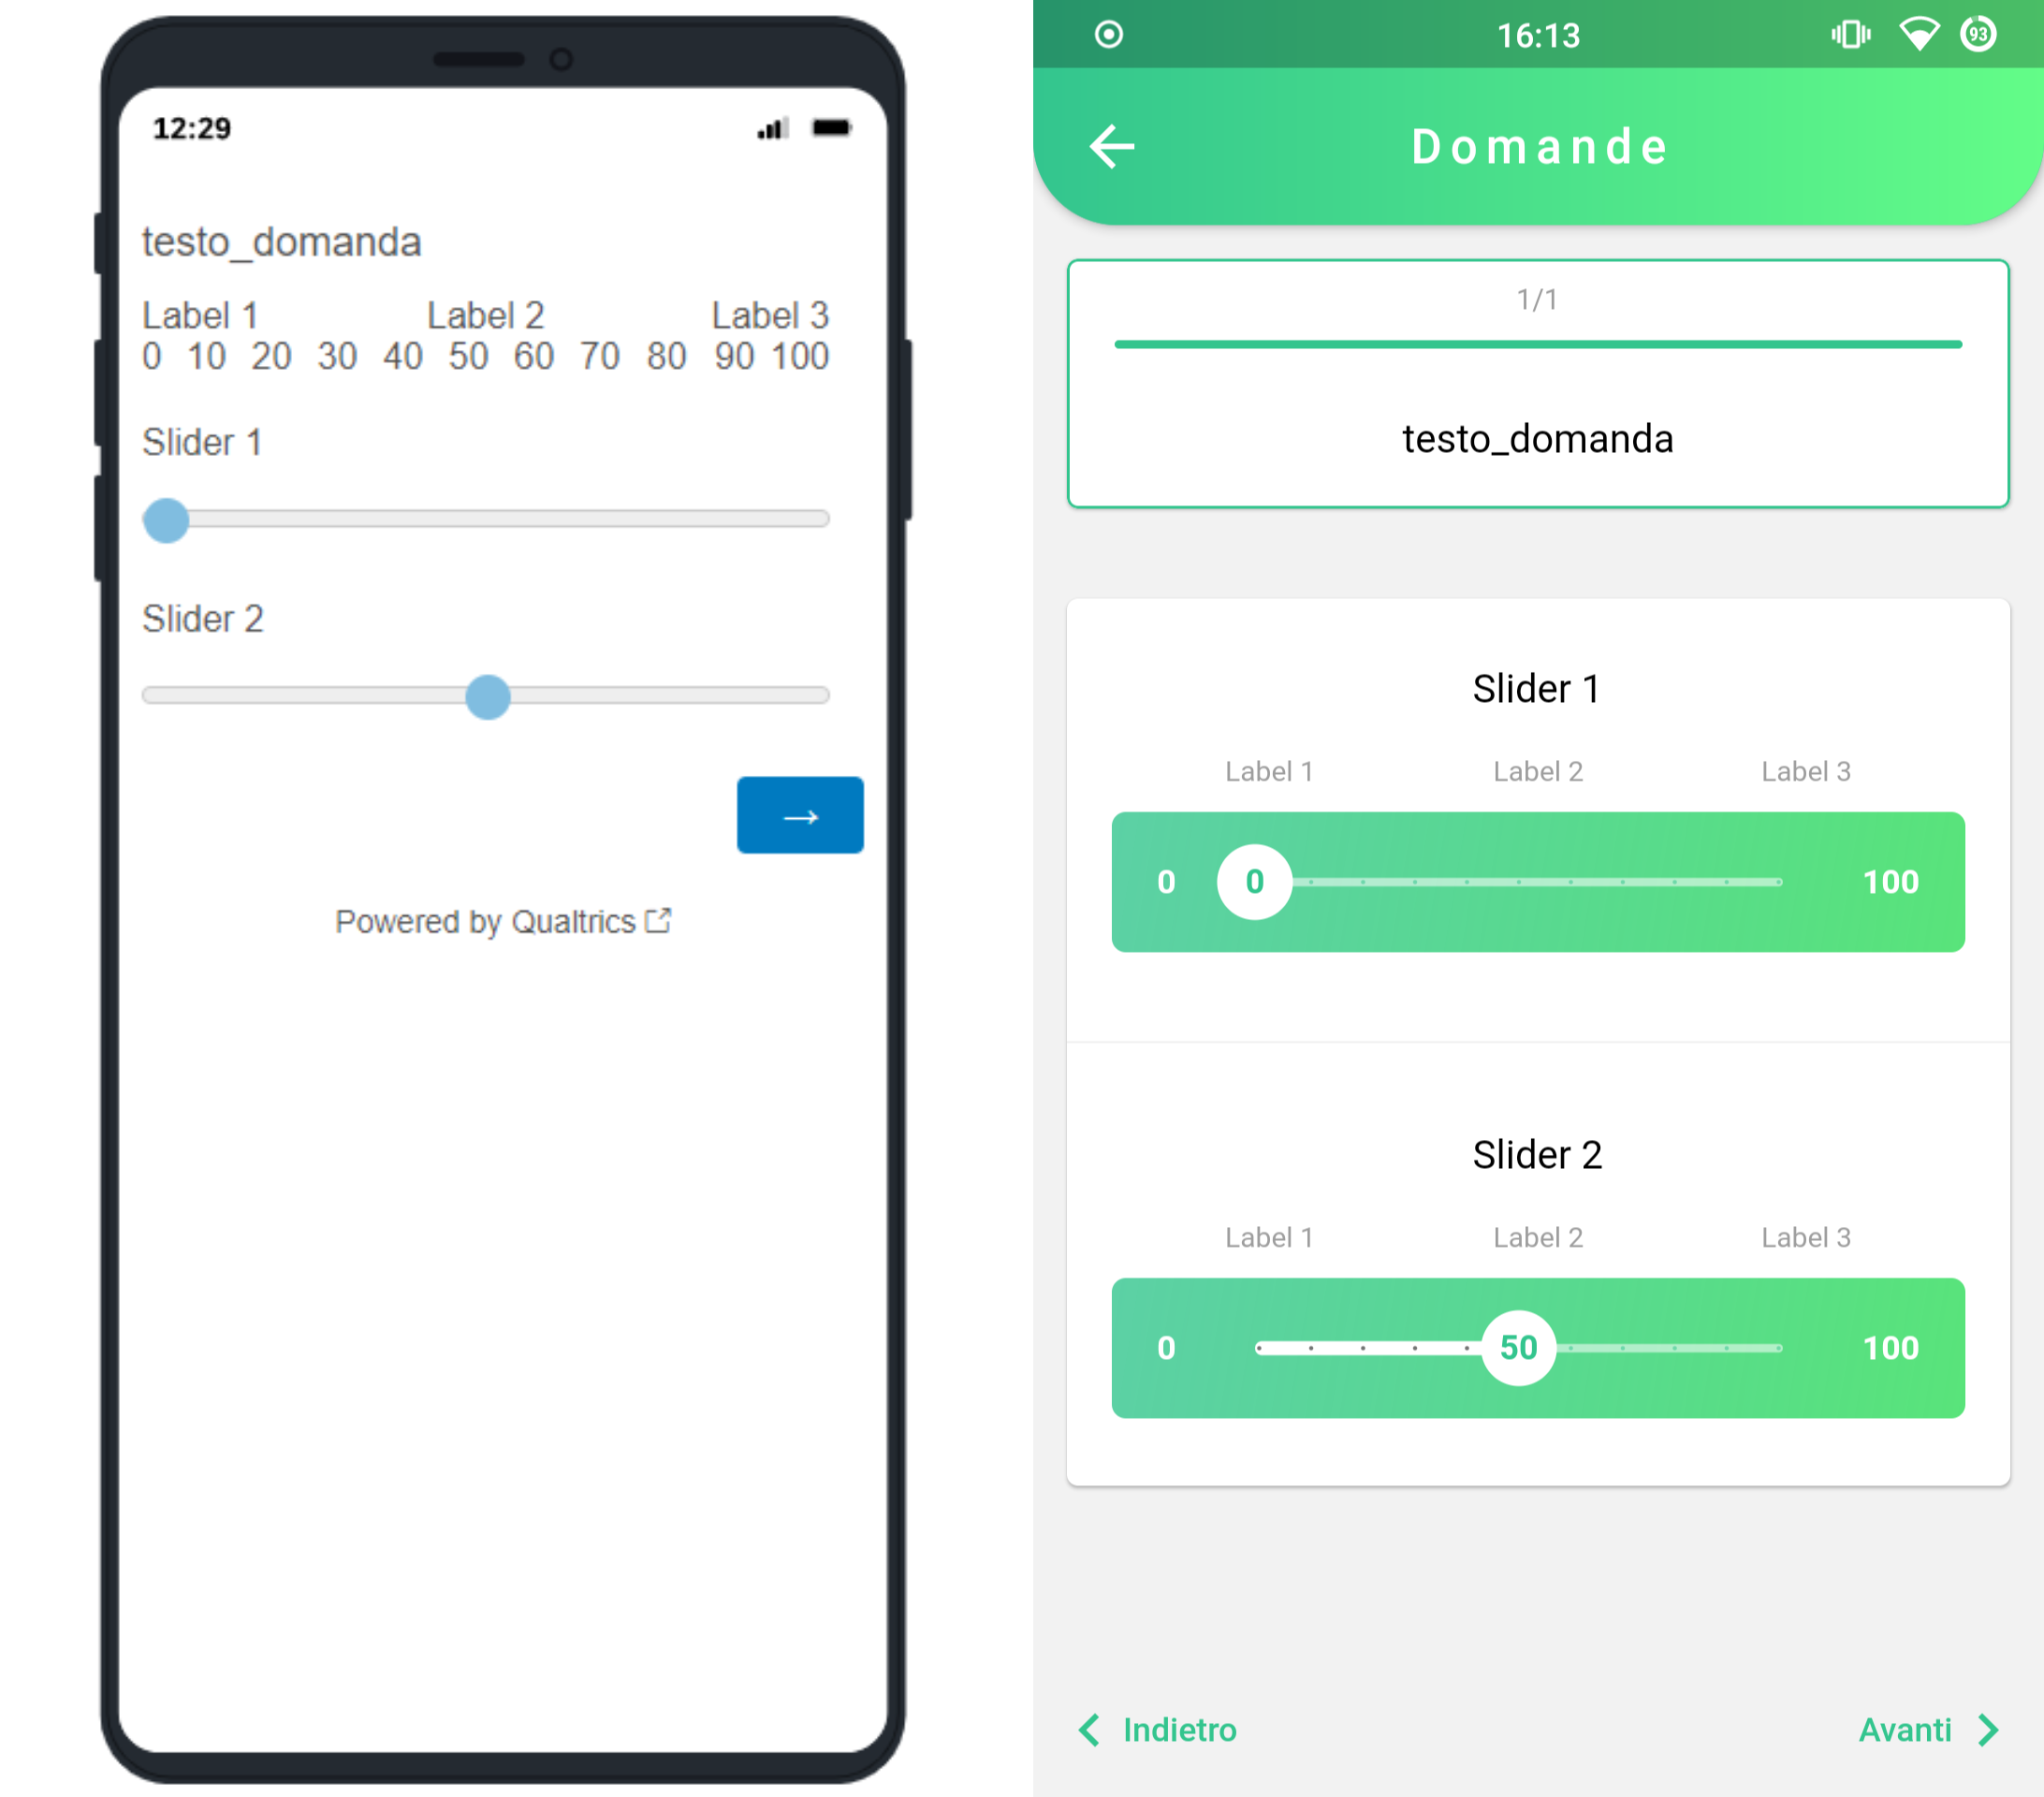
\includegraphics[width=0.7\textwidth]{img/slider}
\caption{Slider}
\label{fig:slider}
\end{figure}

\clearpage
\subsection{Rank Order - "QuestionType": "RO"}
Uno dei tipi di domanda più creativi di Qualtrics è il tipo Rank Order che richiede all'utente, dati degli item, di ordinarli ad esempio per ordine di importanza. Questo ordinamento generalmente viene fatto trascinando gli item l'uno sopra l'altro in una lista: è stato dunque necessario implementare un tipo di lista che permettesse questa interazione. Come possiamo osservare nella \autoref{fig:rank_order}, per evitare ordinamenti accidentali è stato scelto, a differenza di come viene fatto nativamente da Qualtrics, di utilizzare un handler che ricevesse l'input di trascinamento di ogni item. Successivamente, per migliorare ancor di più l'usabilità, è stato scelto di aggiungere anche dei pulsanti che permettessero di scambiare una posizione all'interno della lista in maniera semplice ed efficace. Possiamo osservare la struttura di questa domanda nel \autoref{json:rank_order} e notiamo che di fatto gli item non sono altro che delle \texttt{Choices}.

\subsubsection{Media}
Come visto in precedenza, anche in questo caso è possibile assegnare alle \texttt{Choices} un'immagine e una text entry aggiuntiva.

\subsubsection{Response}
Le risposte a questo tipo di domande sono del tipo \texttt{\{"QuestionID\_ChoiceID": numero\}}, dove numero è il valore intero che rappresenta la posizione nella lista della suddetta choice. Nel caso ci fosse una text entry aggiuntiva, la risposta sarà del tipo \texttt{\{"QuestionID\_ChoiceID\_TEXT": "testo"\}}.

\newpage
\begin{json}
\usemintedstyle[JSON]{trac}
\begin{minted}[]{JSON}
            {
                "QuestionText": "testo_domanda",
                "QuestionID": "QID257",
                "QuestionType": "RO",
                "Choices": {
                    "1": {
                        "Display": "Item 1"
                    },
                    "2": {
                        "Display": "Item 2"
                    },
                    "5": {
                        "Display": "Item 3"
                    }
                },
                "ChoiceOrder": [],
            }
\end{minted}
\caption{Oggetto domanda Rank Order}
\label{json:rank_order}
\end{json}

\begin{figure}[h!]
\centering
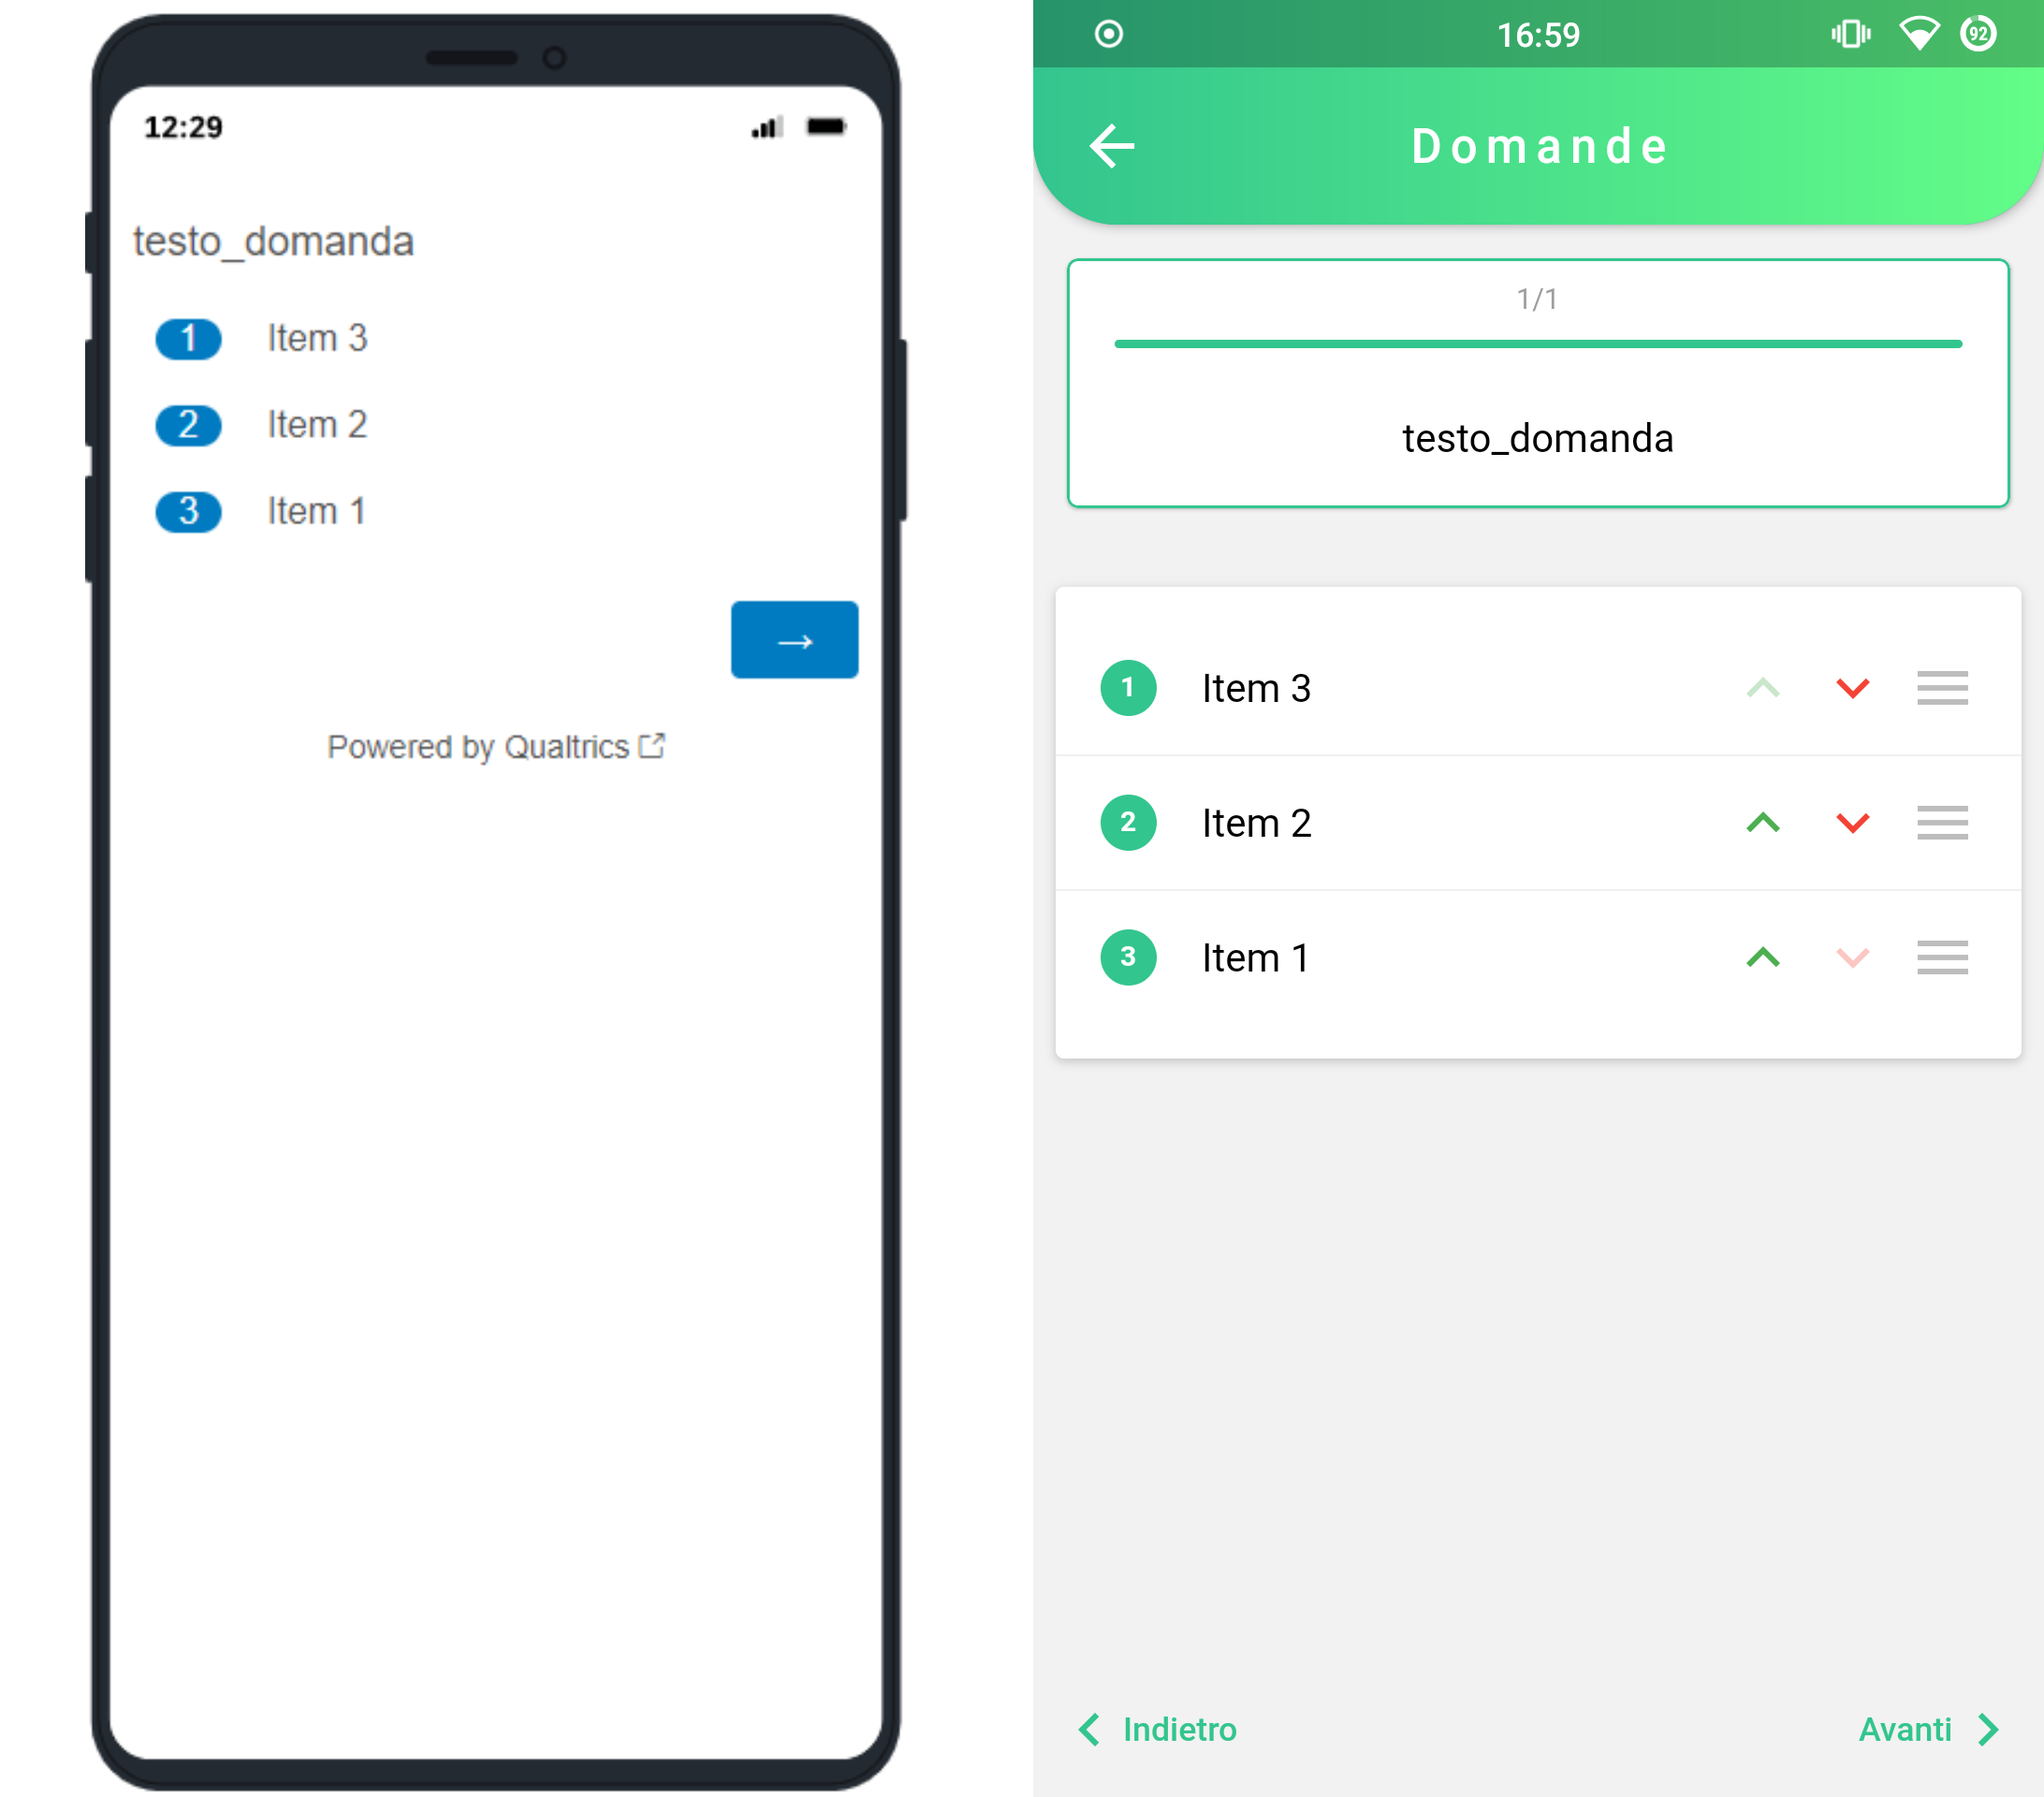
\includegraphics[width=0.66\textwidth]{img/rank_order}
\caption{Rank Order}
\label{fig:rank_order}
\end{figure}

\clearpage
\subsection{Pick, Group and Rank - "QuestionType": "PGR"}
Un'evoluzione delle domande di tipo Rank Order sono le Pick, Group and Rank che sostanzialmente sono sempre delle Rank Order ma con più liste: la domanda richiede, oltre che di ordinare gli item di una lista, di assegnare gli item ad una delle liste disponibili. Come possiamo vedere nella \autoref{fig:PGR}, anche qui sono stati fatti dei cambiamenti per migliorare l'usabilità su mobile: in particolare, per cambiare la lista di un item, non solo è possibile trascinarlo nella lista corrispondente, ma cliccandoci sopra apparirà una finestra di dialogo che permetterà il cambio di lista senza alcun trascinamento. Possiamo osservare la struttura di questo tipo di domanda nel \autoref{json:PGR}; possiamo vedere come sia molto simile alle domande Rank Order con l'aggiunta di un campo \texttt{Groups} che identifica le liste disponibili.

\subsubsection{Media}
Anche in questo caso è possibile assegnare alle \texttt{Choices} un'immagine e una text entry aggiuntiva.

\subsubsection{Response}
Le risposte a questo tipo di domande si suddividono in due parti è sono del tipo \texttt{\{"QuestionID\_index\_GROUP": [ChoiceID\_1, ChoiceID\_2]\}} per indicare quali item fanno parte di quale lista \textit{(o gruppo)} e del tipo\\ \texttt{\{"QuestionID\_Gindex\_ChoiceID\_RANK": numero\}} per indicare l'ordinamento, dove \texttt{Gindex} indica il gruppo di cui fa parte l'item \textit{(ad esempio G0 per il primo gruppo e G1 per il secondo)} e \texttt{numero} indica il rank di quell'item nel suddetto gruppo.
Nel caso ci fosse una text entry aggiuntiva, la risposta sarà del tipo \texttt{\{"QuestionID\_ChoiceID\_TEXT": "testo"\}}.

\newpage
\begin{json}
\usemintedstyle[JSON]{trac}
\begin{minted}[]{JSON}
{
    "QuestionText": "testo_domanda",
    "QuestionID": "QID257",
    "QuestionType": "PGR",
    "Choices": {},
    "ChoiceOrder": [],
    "Groups": [
        "Lista 1",
        "Lista 2"
    ],
}
\end{minted}
\caption{Oggetto domanda Pick, Group and Rank}
\label{json:PGR}
\end{json}

\begin{figure}[h!]
\centering
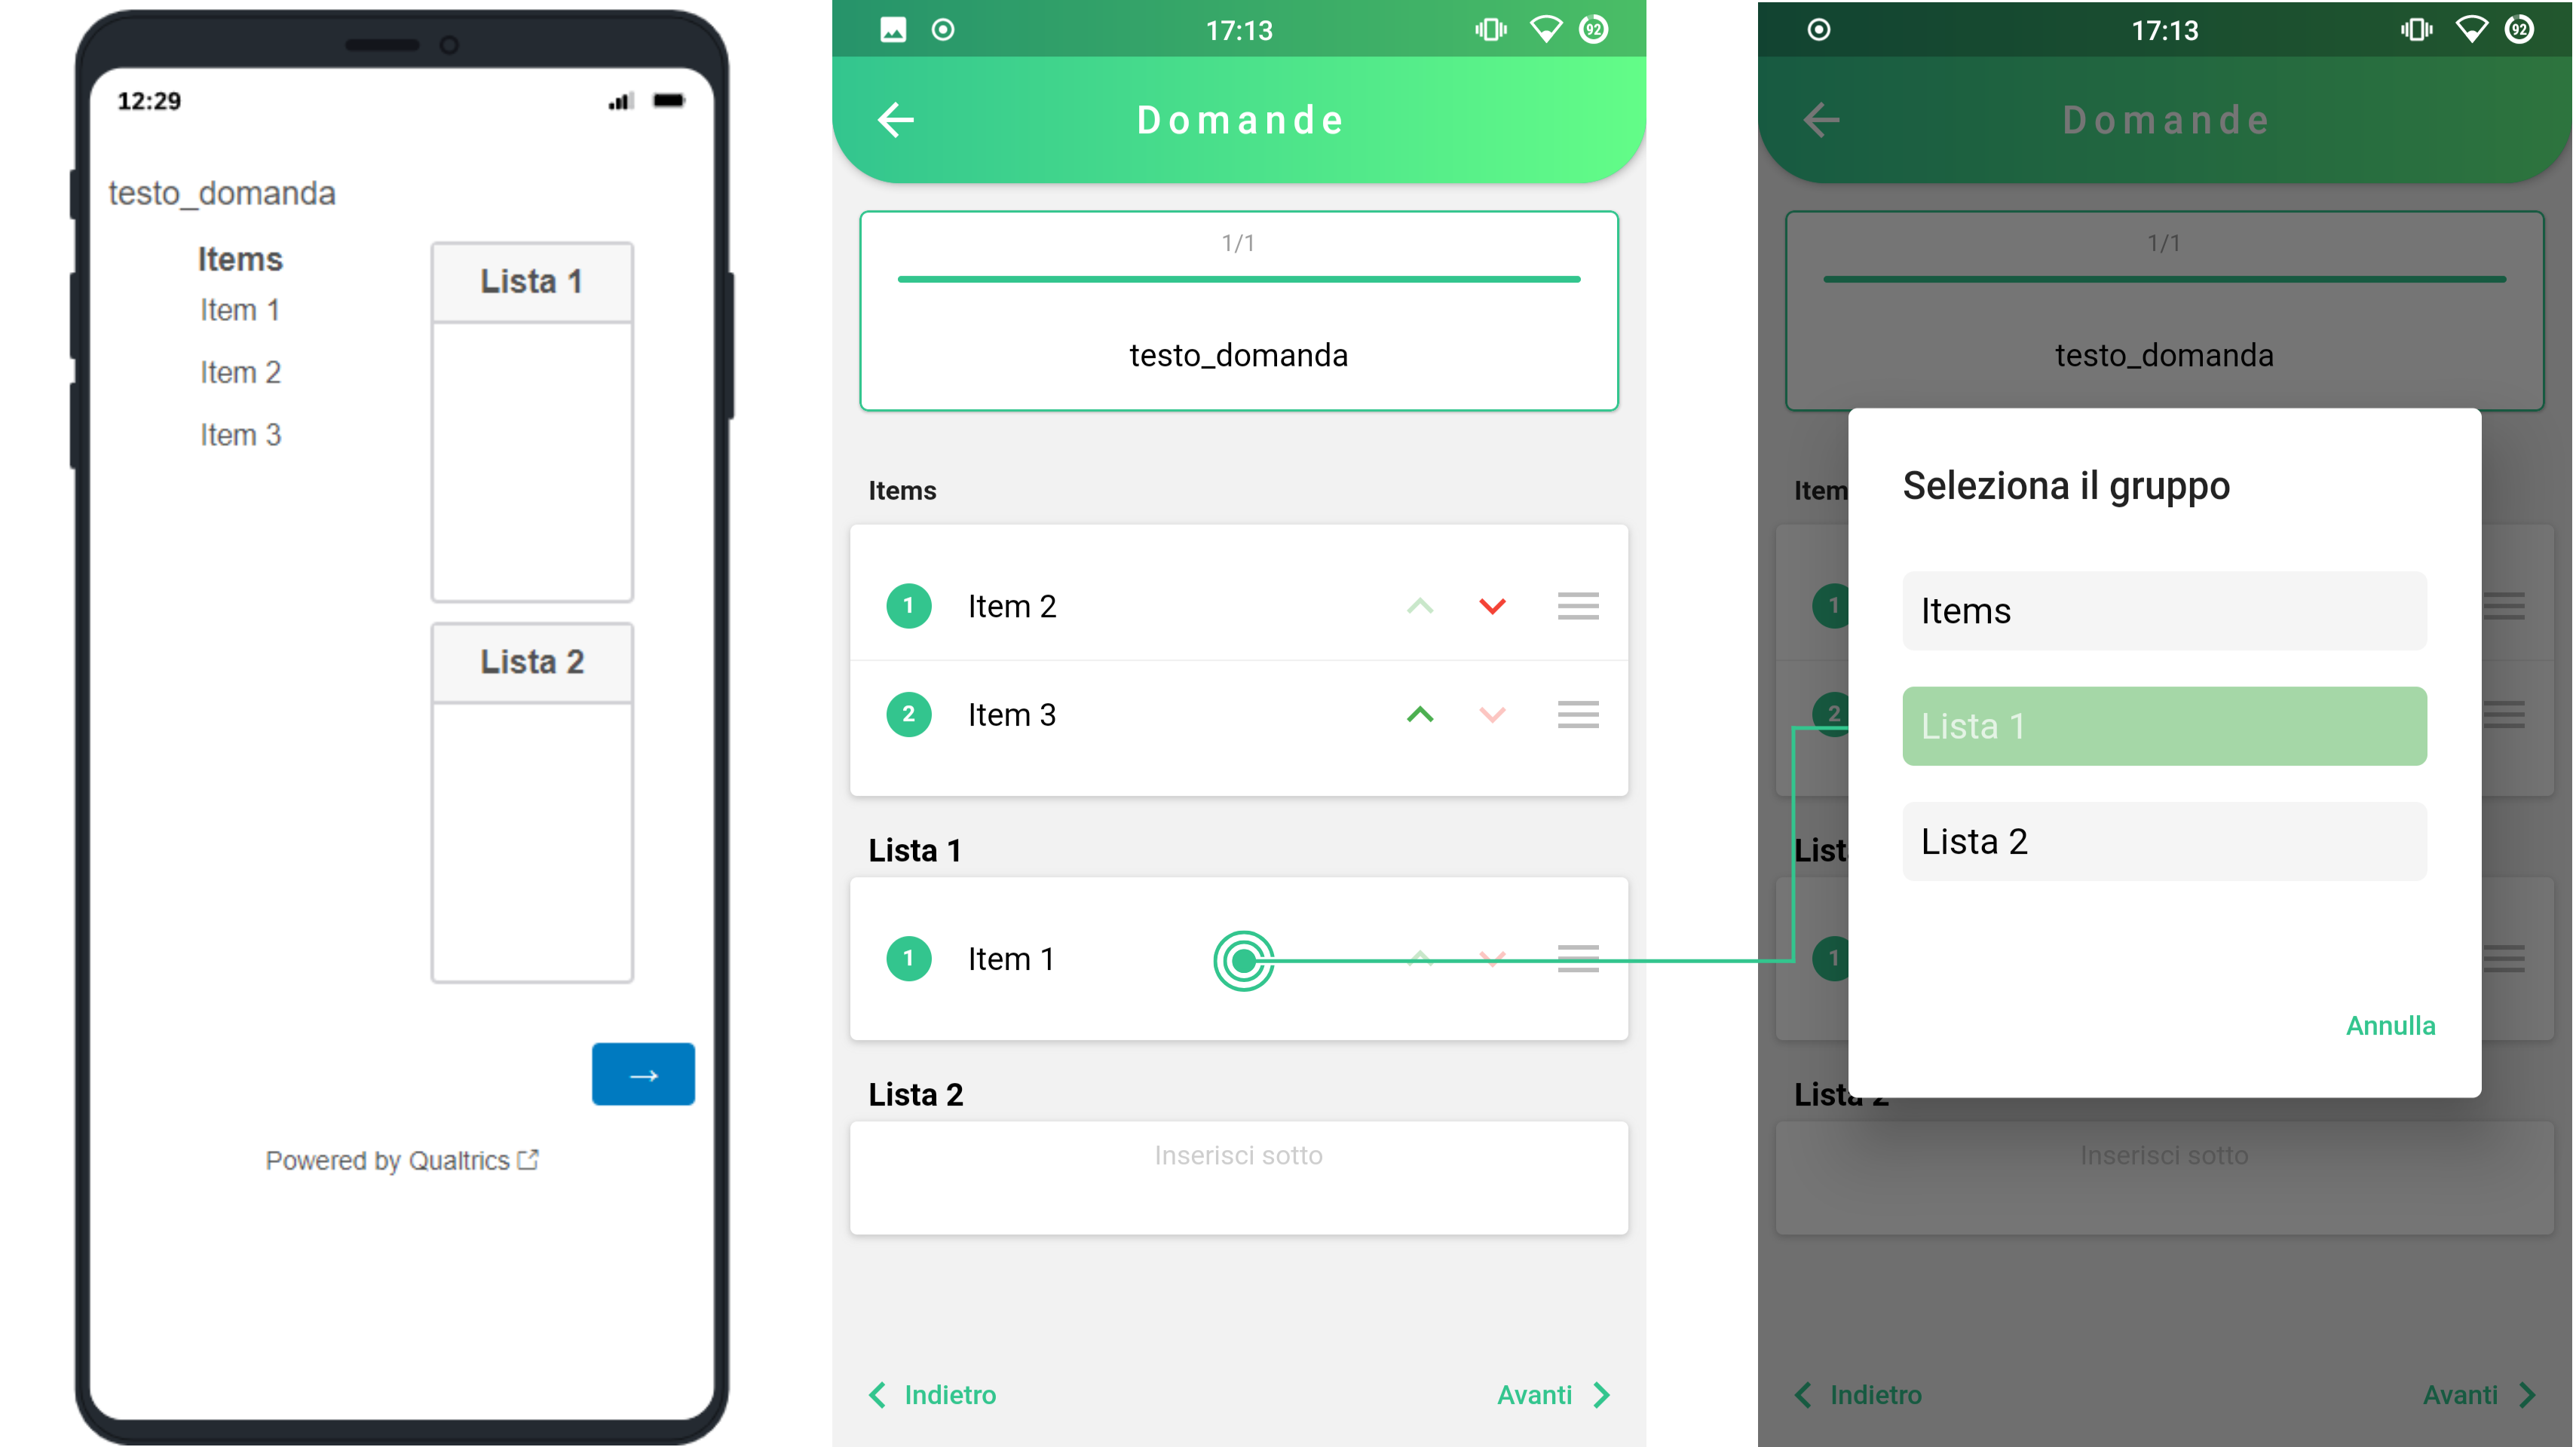
\includegraphics[width=\textwidth]{img/PGR}
\caption{Pick, Group and Rank}
\label{fig:PGR}
\end{figure}

\subsection{Description Box - "QuestionType": "DB"}
Infine, l'ultima entità messa a disposizione da Qualtrics è la Description Box, una "domanda" che contiene solo il testo ed eventualmente dei media \textit{(di cui parleremo nella sezione successiva)}, utile ad esempio per fornire delle spiegazioni all'utente prima che affronti un questionario.

\section{Question Text}
Abbiamo visto nella sezione precedente che c'è un elemento comune a tutte le domande di Qualtrics: tutte presentano un testo di domanda, che a prima vista può sembrare del semplice testo, ma che in realtà è altamente personalizzabile e ha quindi richiesto del codice specifico che lo mostrasse nel modo giusto.

\subsection{Media}
Un aspetto molto utile di questo testo è che Qualtrics permette di inserirvi dei media di accompagnamento come immagini, video e/o audio. A differenza delle domande però, quando viene inserito un media nel testo della domanda questo viene tradotto in un tag \texttt{HTML} adeguato \textit{(in modo che il browser non deva fare nessun lavoro aggiuntivo per visualizzare i media)}; quando viene inserita un'immagine viene creato un tag \texttt{<img src="" />}, per un video viene usato un tag \texttt{<video> <source src="" </source> </video>} mentre per un audio viene usato un tag \texttt{<audio> <source src=""> </source> </audio>}. I tag vengono concatenati all'eventuale plain text.

L'applicazione dunque, prima di mostrare a schermo il testo fornito dalle API, lo analizza in cerca di questi tag e, ogni qual volta ne incontra uno, aggiunge il parametro \texttt{src} ad una lista di sorgenti in base al media da mostrare. Successivamente, utilizzando delle espressioni regolari, l'applicazione elimina completamente i tag media dal testo, in modo che non vengano poi mostrati a schermo. A questo punto, utilizzando le liste di sorgenti siamo in grado di renderizzare i media desiderati insieme al testo "pulito". Possiamo osservare alcuni media nella \autoref{fig:media_vari}.

\begin{figure}[h!]
\centering
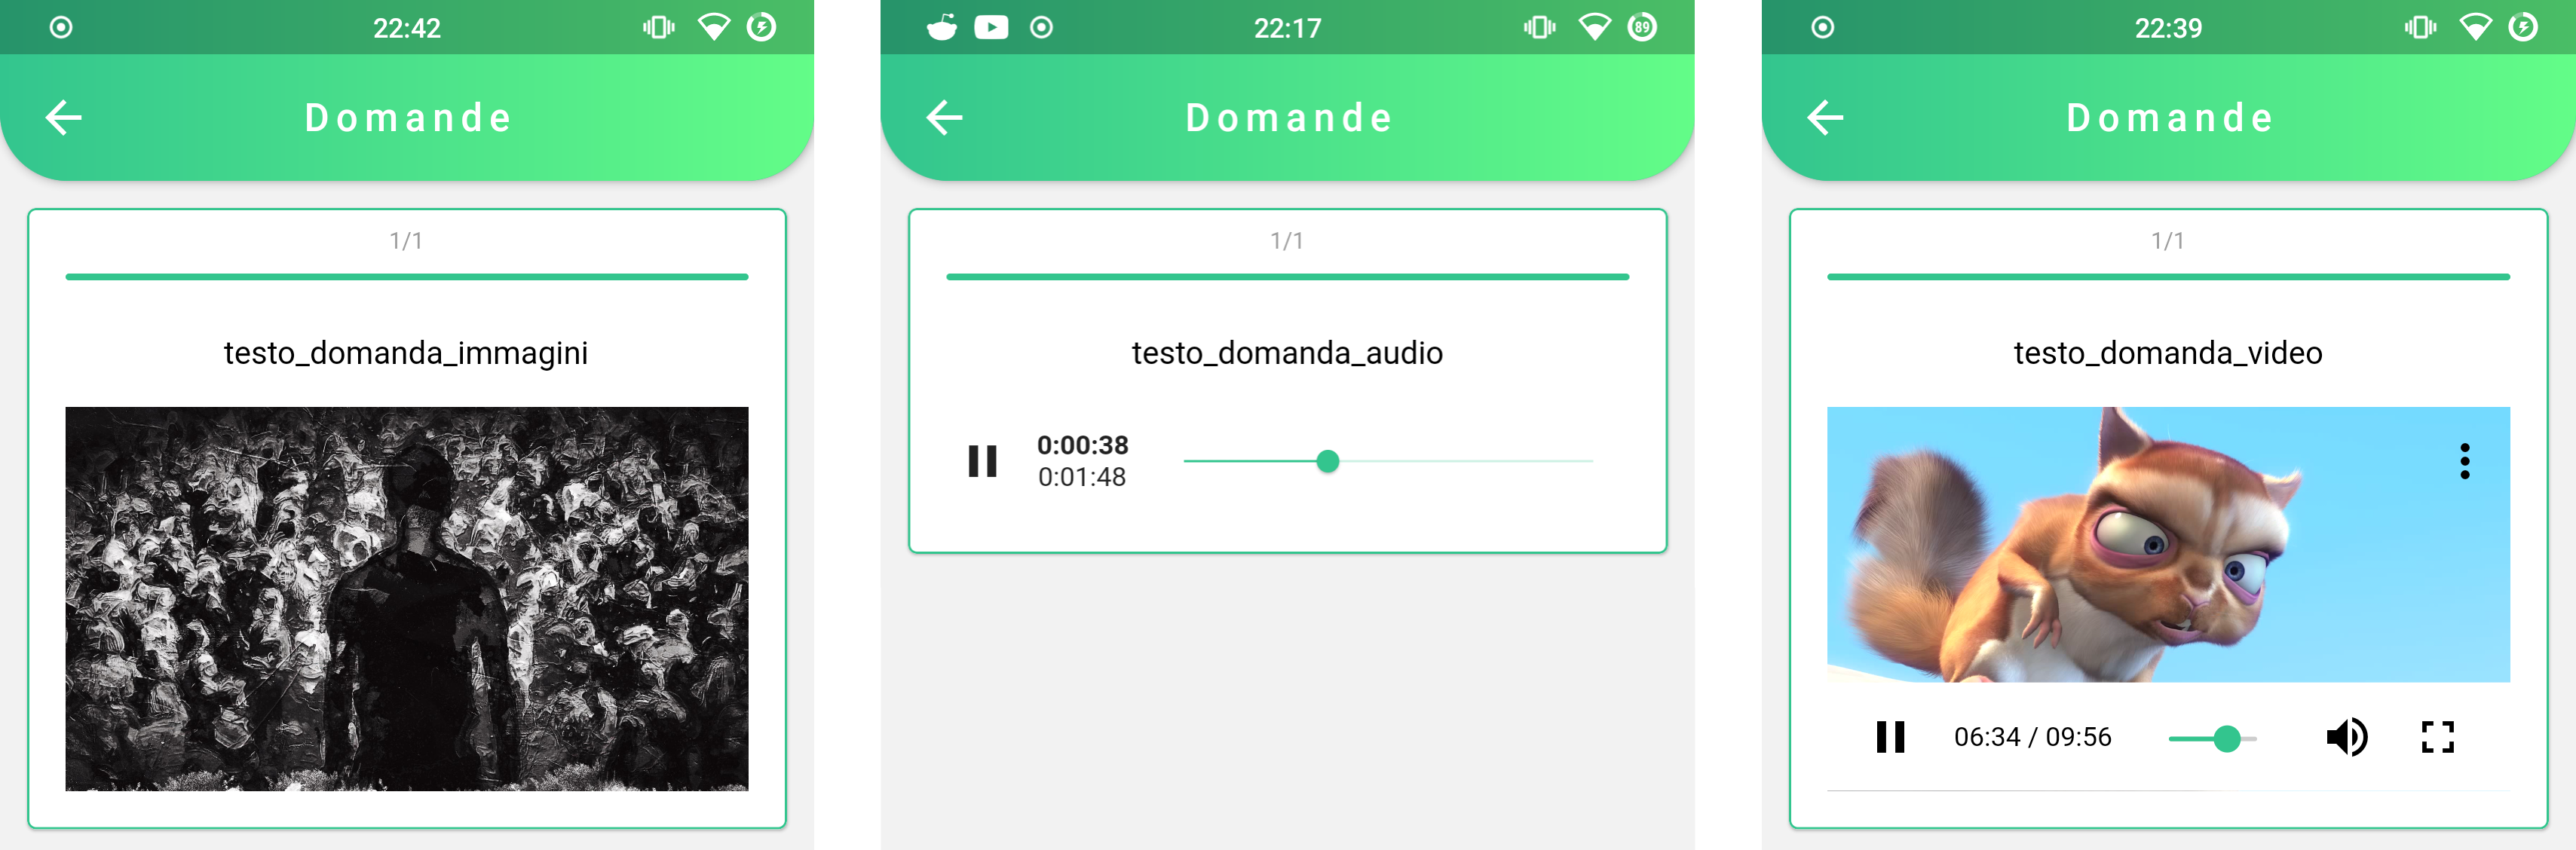
\includegraphics[width=0.95\textwidth]{img/media_vari}
\caption{Vari media nel question text}
\label{fig:media_vari}
\end{figure}

\subsection{YouTube support}
Purtroppo, per quanto riguarda i video, Qualtrics offre poco spazio di archiviazione e la soluzione è caricare i video in un file server dal quale ottenere il link allo stream diretto \textit{(e creando i tag video di prima)}, oppure caricare i vari video su YouTube, inserendo un iframe nella domanda. Sfortunatamente, di base i link di YouTube non sono link diretti allo stream video e di conseguenza non funzionano col lettore video utilizzato per quel tipo di link \textit{(anche se sono ottenibili tramite procedure non ovvie, ma sono stream separati per audio e video e non ho la sicurezza che siano in linea con i termini d'uso di YouTube)}. La soluzione è stata utilizzare un iframe vero e proprio anche nell'applicazione, seppur leggermente mascherato per avere un aspetto più nativo.

\subsection{Rich Text Editor}
Qualtrics permette inoltre di modificare il testo della domanda tramite un rich text editor, ovvero tramite un editor che permette di assegnare dello stile al testo che può essere grassetto, corsivo, sottolineato ma anche colorato, con lo sfondo colorato, in elenco puntato e così via. Questo è il motivo per il quale, in tutti gli screen visti fino ad ora, il testo appare "semplice": la scelta di modificarlo e dargli enfasi è stata lasciata a chi crea le domande, mentre l'applicazione ricrea tale stile.
Per realizzare tutto ciò è stato seguito un approccio simile a quello per i media: per creare questi stili vengono utilizzati dei tag \texttt{HTML} che l'applicazione individua e, utilizzando un widget di tipo \texttt{RichText}, che permette di avere diversi widget \texttt{TextSpan} con diversi stili di testo ciascuno, ricrea lo stile desiderato eliminando dal testo poi i tag. Possiamo osservare un esempio di testo editato nella \autoref{fig:rich_text}.

\begin{figure}[h!]
\centering
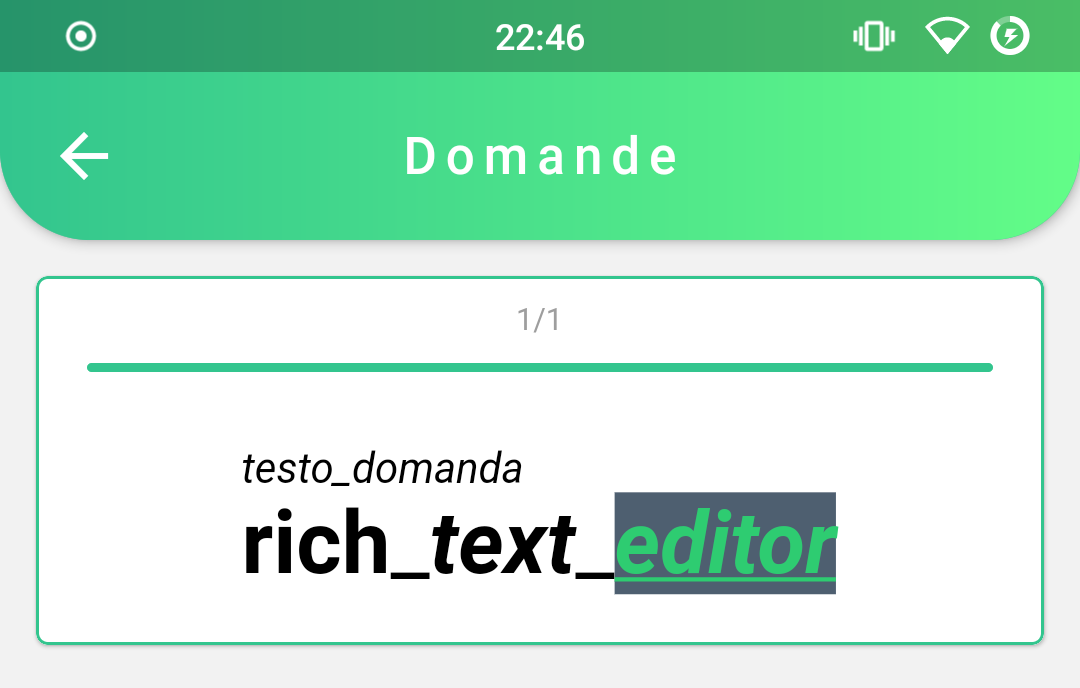
\includegraphics[width=0.5\textwidth]{img/rich_text}
\caption{Esempio di testo editato}
\label{fig:rich_text}
\end{figure}

\section{Validation}
Quando abbiamo parlato di domande abbiamo visto che un altro parametro comune a tutte è la cosiddetta \texttt{Validation}: questo oggetto contiene una serie di regole logiche \textit{(definibili da chi crea le domande tramite l'ambiente Qualtrics)} che definiscono se una certa risposta è giusta o meno. Queste regole sono varie e possono definire delle risposte che devono essere scelte, risposte che non devono essere scelte, un numero minimo di scelte e così via. Un esempio di validation è visibile nel \autoref{json:validation}.

\begin{json}
\usemintedstyle[JSON]{trac}
\begin{minted}[]{JSON}
"Validation": {
    "Logic": {
        "0": {
            "0": {
                "QuestionID": "QID162",
                "Operator": "Selected",
                "LeftOperand": "q://QID162/SelectableChoice/1",
            },
            "1": {
                "QuestionID": "QID162",
                "Operator": "EqualTo",
                "LeftOperand": "q://QID162/SelectedChoicesCount",
                "RightOperand": "1",
                "Conjuction": "And"
            },
            "2": {
                "QuestionID": "QID162",
                "Operator": "GreaterThanOrEqual",
                "QuestionIDFromLocator": "QID162",
                "LeftOperand": "q://QID162/SelectedChoicesCount",
                "RightOperand": "2",
                "Conjuction": "Or"
            },
        },
    },
}
\end{minted}
\caption{Esempio di oggetto Validation}
\label{json:validation}
\end{json}

\subsection{Struttura dati e traduzione}
Possiamo notare come le regole logiche siano identificate da un \texttt{Operator}, che stabilisce cosa va controllato, e da degli operandi: il \texttt{LeftOperand} in particolare è un hyperlink ad un opzione di una domanda piuttosto che al numero di opzioni selezionate e così via da cui però è deducibile a cosa si riferisce. L'applicazione, leggendo l'operatore e gli operandi potrà sapere cosa deve controllare per validare una risposta.

Notiamo però che le regole possono essere multiple e sono legate fra loro da una \texttt{Conjuction}, ovvero da un operatore logico che può essere AND oppure OR: è necessario che l'applicazione valuti l'intero set di regole per poter valutare una risposta. È necessaria dunque una struttura dati che venga valutata implicitamente dall'applicazione.

Ancora una volta sono tornate utili le mappe: ad ogni domanda munita di validation sarebbe stata associata una mappa che al suo interno avrebbe contenuto altre mappe. In particolare, al livello più esterno viene usato come chiave l'id della domanda alla quale è legata la regola e come valore è presente un'altra mappa che come chiave ha una \textbf{posizione}; la posizione determina quali regole sono da considerarsi insieme e quali no. La valutazione implicita viene eseguita qui: tutte le regole con la stessa posizione sono valutate come se fossero in AND logico, mentre tutte le regole con posizione diversa sono valutate in OR logico.
Sotto alle posizioni ci sono poi delle ulteriori mappe che hanno come chiave l'operatore che identifica il tipo di controllo da eseguire e come valore un oggetto con due valori: un \texttt{access} che identifica il \texttt{LeftOperand} \textit{(è la chiave d'accesso alla mappa delle risposte che ritorna il valore da controllare)} e un \texttt{RightOperand} che può essere un numero, del testo o una lista di id di opzioni, a seconda anche dell'operatore utilizzato.

Gli operatori disponibili \textit{(e quindi le chiavi delle mappe più interne)} sono diversi e ognuno implementa un certo tipo di controllo. 

Alcuni operatori sono:
\begin{itemize}
\item \textbf{whitelist} - contiene le scelte che devono essere selezionate
\item \textbf{blacklist} - contiene le scelte che non devono essere selezionate
\item \textbf{minChoices} - almeno \textit{n} scelte selezionate
\item \textbf{maxChoices} - al massimo \textit{n} scelte selezionate
\item \textbf{notEqualLength} - selezionate un numero $\neq$ \textit{n} di scelte
\item \textbf{equalLength} - selezionate esattamente \textit{n} scelte
\item \textbf{equal} - la risposta in corrispondenza della accessKey è uguale al rightOperand
\item \textbf{greaterThanLength} - selezionate un numero > \textit{n} di scelte
\item \textbf{greaterThanEqualLength} - selezionate un numero $\geq$ \textit{n} di scelte
\item \textbf{lessThanLength} - selezionate un numero < \textit{n} di scelte
\item \textbf{lessThanEqualLength} - selezionate un numero $\leq$ \textit{n} di scelte
\end{itemize}

In particolare, l'esempio visto nel \autoref{json:validation} viene tradotto nella struttura visibile nel \autoref{json:validation_tradotta}, ovvero considera in AND le regole \textbf{whitelist} \textit{(must be selected)} e \textbf{equalLength} \textit{(devono esserne selezionate esattamente n)} che hanno come posizione 0, il tutto considerato poi in OR con la regola \textbf{greaterThanEqualLength} \textit{(devono esserne selezionate un numero >= n)} che ha posizione 1.

\begin{json}
\usemintedstyle[JSON]{trac}
\begin{minted}[]{JSON}
"QID162": {
    0: {
        "whitelist": {
            "access": "QID162",
            "rightOperand": [1]
        },
        "equalLength": {
            "access": "QID162",
            "rightOperand": 1
        }
    },
    1: {
        "greaterThanEqualLength": {
        "access": "QID162",
        "rightOperand": 2
        },
    },
}
\end{minted}
\caption{Esempio di mappa di regole logiche}
\label{json:validation_tradotta}
\end{json}

\subsection{Risposta in app}
Per gestire la struttura dati di validazione, che è condivisa fra le varie domande, è stato creato un \texttt{provider} che permettesse così di aggiungere le regole in fase di lettura delle domande dalle API e di consultarle in fase di controllo. In particolare, se il controllo fallisce l'applicazione evidenzia la domanda con un alone rosso come possiamo osservare nella \autoref{fig:validation_errata}.

\begin{figure}[h!]
\centering
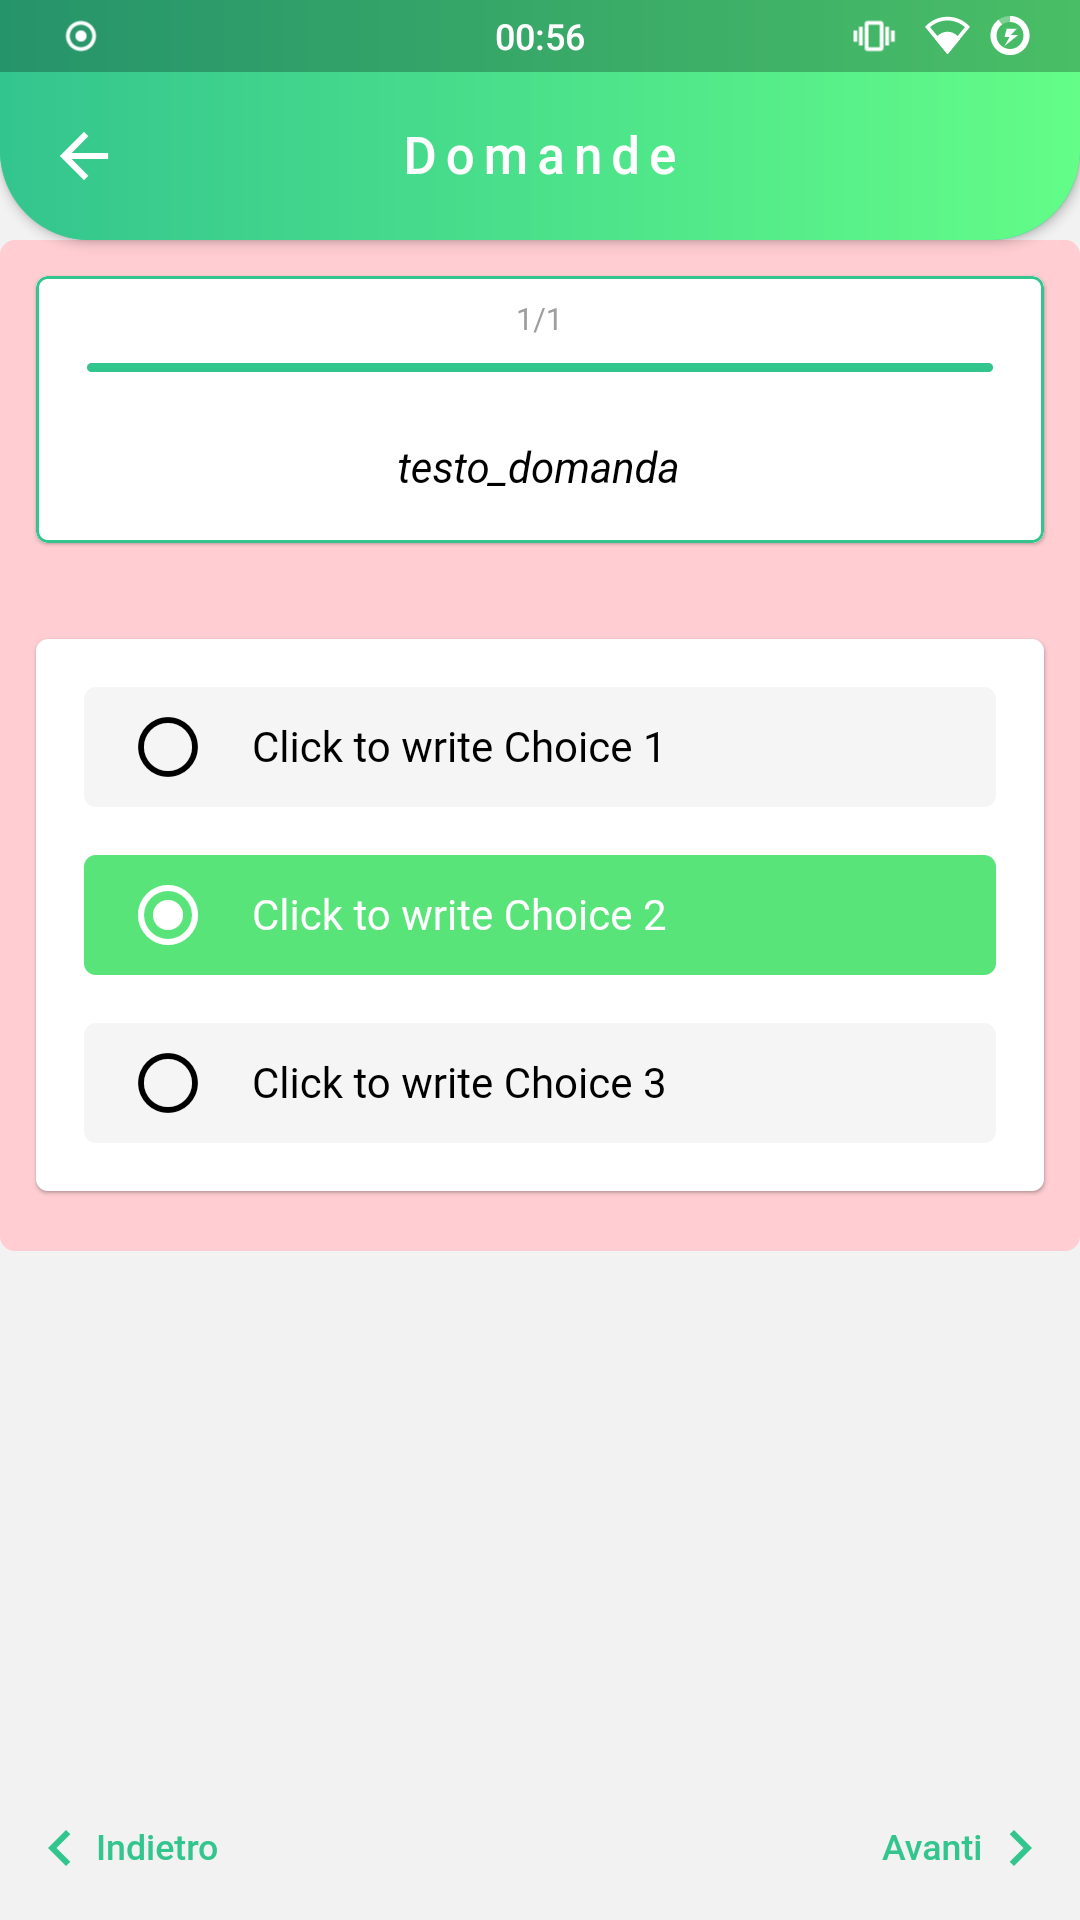
\includegraphics[width=0.7\textwidth]{img/validation_errata}
\caption{Esempio di validazione errata}
\label{fig:validation_errata}
\end{figure}

\newpage
\section{Screening}
Nel capitolo precedente abbiamo parlato di una fase iniziale di screening atta a individuare le patologie di cui potenzialmente soffre l'utente: questi screening sono composti sia da alcune domande generiche \textit{(domande sociodemografiche)} che da specifiche domande misurabili che diano un'idea dei problemi del paziente. La particolarità di questo processo è che i tipi di domande e le scale utilizzate sono varie a seconda della patologia e sono basati su test psicologici ufficiali e ben noti e producono un risultato che collochi ogni patologia in una determinata fascia di rischio tra \textbf{minimo}, \textbf{lieve}, \textbf{moderato} e \textbf{alto}.

Per mantenere il livello di ogni patologia verrà utilizzato un provider apposito che fornisca al resto dell'applicazione le informazioni su quali sono i moduli da trattare.
Inoltre, poiché gli screening vengono erogati tutti in una sola sessione, per la loro organizzazione si è scelto di creare un unico sondaggio che contenesse vari blocchi, ognuno dei quali si riferisce ad uno specifico screening: in questo modo l'applicazione può distinguere tra i vari screening e calcolarne il punteggio indipendentemente dagli altri. Inoltre, in questo modo verrà inviata una sola risposta al server di Qualtrics una volta che l'utente ha completato gli screening.

\subsection{Depressione}
Per misurare il livello di depressione viene utilizzata la scala \textbf{Beck Depression Inventory-II \textit{(BDI-II)}}\cite{BDI-II} che consiste di 21 domande \textit{(anche dette items)}, ognuna delle quali può assumere un punteggio che va da 0 a 3 in base alla risposta data.
Il punteggio finale, ottenuto sommando i punteggi di tutte e 21 le domande, indicherà la fascia di rischio della suddetta patologia, in particolare:
\begin{itemize}
\item \textbf{[0, 13]} Indica un rischio minimo
\item \textbf{[14, 19]} Indica un rischio lieve
\item \textbf{[20, 28]} Indica un rischio moderato
\item \textbf{[29, 63]} Indica un rischio alto
\end{itemize}

Fanno eccezione alcune domande trasversali, il quale punteggio, se alto, influenza anche il rilevamento di altre patologie come le problematiche del sonno e dell'ansia.
Per semplificare l'ottenimento di tali punteggi, le risposte alle varie domande iniziano con "\texttt{x}. " dove \texttt{x} indica il punteggio relativo alla risposta.

\subsection{Ansia}
Per l'ansia, la scala utilizzata è la \textbf{State-Trait  Anxiety Inventory \textit{(STAI)}}\cite{STAI} che consiste di 40 domande che accettano come risposta una scala Likert a 4 punti. La scala STAI si suddivide in due sotto-scale: \textbf{SAI} e \textbf{TAI} utili a misurare l'\textbf{ansia di stato} \textit{(ansia legata ad un evento)} e l'\textbf{ansia di tratto} \textit{(ansia legata alle caratteristiche personali)}.

Di conseguenza, le domande si suddividono in 20 per la scala SAI e 20 per la scala TAI ed il punteggio minimo è di 20 per ciascuna scala \textit{(la scala likert utilizzata va da 1 a 4)}.\\
Occorre notare però che entrambe le sotto-scale presentano domande legate sia alla presenza che all'assenza di ansia. Di conseguenza alcuni item sono invertiti \textit{(es: "Mi sento calmo: 4" vale 1)}: vale a dire che il punteggio degli item legati all'assenza di ansia è l'inverso della risposta data.

Le rispettive fasce di rischio per le due scale sono:
\begin{itemize}
\item \textbf{[0, 40]} Indica un rischio minimo
\item \textbf{[41, 50]} Indica un rischio lieve
\item \textbf{[51, 60]} Indica un rischio moderato
\item \textbf{[60, 80]} Indica un rischio alto
\end{itemize}

La sotto-scala col rischio maggiore determinerà quindi la fascia legata all'ansia nell'applicazione.

In questo caso la risposta stessa è il punteggio \textit{(tranne per quando si tratta di domande invertite, risolvibile comunque con un'operazione di modulo)} e non sono necessarie ulteriori azioni per ricavarlo.

\newpage
\subsection{Problemi di sonno}
Per calcolare le problematiche del sonno viene utilizzata la \textbf{Pittsburgh Sleep Quality Index \textit{(PSQI)}}\cite{PSQI} che consiste di 19 item raggruppati in 7 componenti a cui viene assegnato un punteggio da 0 a 3. Per ottenere tale punteggio bisogna considerare i punteggi, sempre da 0 a 3, associati agli item facenti parte della relativa componente. Il punteggio massimo è quindi di 21 \textit{(vengono considerati i punteggi delle componenti per la scala)} e le fasce di rischio sono:
\begin{itemize}
\item \textbf{[0, 4]} Indica un rischio minimo
\item \textbf{[5, 10]} Indica un rischio lieve
\item \textbf{[10, 15]} Indica un rischio moderato
\item \textbf{[15, 21]} Indica un rischio alto
\end{itemize}

In questo caso le domande sono di vario tipo: alcune utilizzano una scala likert che fornisce direttamente il punteggio mentre altre richiedono all'utente di inserire, ad esempio, le ore di sonno dalle quali poi ricavare un punteggio.

\subsection{Dolore cronico}
Per calcolare la fascia di rischio del dolore cronico viene utilizzata la scala \textbf{Brief Pain Inventory \textit{(BPI)}}\cite{BPI} che consiste di due sotto-scale, la prima relativa all'\textbf{intensità del dolore} composta da 4 item e la seconda relativa all'\textbf{interferenza del dolore} composta da 11 item. Tutti gli item sono valutati tramite una scala likert a 11 punti \textit{(da 0 a 10)}. Ognuna delle due scale può assumere un punteggio da 0 a 10 e la fascia della patologia viene decisa dalla scala con punteggio maggiore.

In particolare, le fasce di rischio sono:
\begin{itemize}
\item \textbf{[0, 4]} Indica un rischio minimo
\item \textbf{[5, 6]} Indica un rischio lieve
\item \textbf{[7, 8]} Indica un rischio moderato
\item \textbf{[9, 10]} Indica un rischio alto
\end{itemize}

\subsection{Burnout}
Il rischio di burnout viene calcolato tramite la scala \textbf{School Burnout Inventory \textit{(SBI)}}\cite{SBI} che si suddivide in tre sotto-scale: \textbf{Esaurimento a scuola}, \textbf{Cinismo verso la scuola} e  \textbf{Senso di inadeguatezza a scuola}, ognuna delle quali contiene degli item valutati con una scala likert da 1 a 6 il cui punteggio totale va poi suddiviso per il numero di item della sotto-scala stessa. Il punteggio va poi confrontato con degli indici di un campione italiano di studenti in base al sesso dell'utente.

Le fasce di rischio sono quindi selezionate in base al sesso dell'utente e alla sotto-scala con punteggio maggiore come possiamo vedere nella \autoref{table:sbi}.
\setlength\arrayrulewidth{1pt}
\definecolor{Lines}{gray}{0.3}
\definecolor{Gray}{gray}{0.9}
\definecolor{None}{rgb}{1, 1, 1}
\definecolor{Minimo}{HTML}{FDEDED}
\definecolor{Lieve}{HTML}{F9C8C8}
\definecolor{Moderato}{HTML}{F5A3A3}
\definecolor{Alto}{HTML}{F17E7E}

\newcolumntype{M}[1]{>{\centering\arraybackslash}m{#1}}

\begin{table}[h!]
\def\arraystretch{1.5}
\begin{center}
\begin{tabular}{| m{80pt} | M{60pt} | M{60pt} | M{90pt} | M{60pt} |}
 \arrayrulecolor{Lines}\hline
 \rowcolor{Gray}
 \textbf{MASCHI} &
 \textbf{MINIMO} &
 \textbf{LIEVE} &
 \textbf{MODERATO} &
 \textbf{ALTO} \\
 \hline
 \cellcolor{None} Esaurimento& \cellcolor{Minimo} 1 - 2.91 & \cellcolor{Lieve} 2.92 - 3.612 & \cellcolor{Moderato} 3.613 - 4.306 & \cellcolor{Alto} 4.307 - 5 \\
 \hline
 \cellcolor{None} Cinismo& \cellcolor{Minimo} 1 - 3.16 & \cellcolor{Lieve} 3.17 - 3.77 & \cellcolor{Moderato} 3.78 - 4.39 & \cellcolor{Alto} 4.40 - 5 \\
 \hline
 \cellcolor{None} Inadeguatezza& \cellcolor{Minimo} 1 - 3.22 & \cellcolor{Lieve} 3.23 - 3.82 & \cellcolor{Moderato} 3.83 - 4.40 & \cellcolor{Alto} 4.41 - 5 \\
 \hline
\end{tabular}
\end{center}

\bigskip
\begin{center}
\begin{tabular}{| m{80pt} | M{60pt} | M{60pt} | M{90pt} | M{60pt} |}
 \arrayrulecolor{Lines}\hline
 \rowcolor{Gray}
 \textbf{FEMMINE} & \textbf{MINIMO} & \textbf{LIEVE} & \textbf{MODERATO} & \textbf{ALTO} \\
 \hline
 \cellcolor{None} Esaurimento& \cellcolor{Minimo} 1 - 3.04 & \cellcolor{Lieve} 3.05 - 3.6 & \cellcolor{Moderato} 3.7 - 4.34 & \cellcolor{Alto} 4.35 - 5 \\
 \hline
 \cellcolor{None} Cinismo&\cellcolor{Minimo} 1 - 3.05 & \cellcolor{Lieve} 3.06 - 3.706 & \cellcolor{Moderato} 3.707 - 4.352 & \cellcolor{Alto} 4.353 - 5 \\
 \hline
 \cellcolor{None} Inadeguatezza&\cellcolor{Minimo} 1 - 3.11 & \cellcolor{Lieve} 3.12 - 3.745 & \cellcolor{Moderato} 3.746 - 4.372 & \cellcolor{Alto} 4.373 - 5 \\
 \hline
\end{tabular}
\end{center}

\bigskip
\begin{center}
\begin{tabular}{| m{80pt} | M{60pt} | M{60pt} | M{90pt} | M{60pt} |}
 \arrayrulecolor{Lines}\hline
 \rowcolor{Gray}
 \textbf{ALTRO} & \textbf{MINIMO} & \textbf{LIEVE} & \textbf{MODERATO} & \textbf{ALTO} \\
 \hline
 \cellcolor{None} Esaurimento& \cellcolor{Minimo} 1 - 2.97 & \cellcolor{Lieve} 2.98 - 3.606 & \cellcolor{Moderato} 3.607 - 4.323 & \cellcolor{Alto} 4.234 - 5 \\
 \hline
 \cellcolor{None} Cinismo& \cellcolor{Minimo} 1 - 3.10 & \cellcolor{Lieve} 3.11 - 3.73 & \cellcolor{Moderato} 3.74 - 4.37 & \cellcolor{Alto} 4.38 - 5 \\
 \hline
 \cellcolor{None} Inadeguatezza& \cellcolor{Minimo} 1 - 3.16 & \cellcolor{Lieve} 3.17 - 3.78 & \cellcolor{Moderato} 3.79 - 4.38 & \cellcolor{Alto} 4.39 - 5 \\
 \hline
\end{tabular}
\end{center}
\caption{Tabella fasce di rischio SBI}
\label{table:sbi}
\end{table}

\newpage
\subsection{Pensieri autodistruttivi}
Per il calcolo della fascia dei pensieri autodistruttivi viene usata la \textbf{Columbia-Suicide Severity Rating Scale \textit{(C-SSRS)}}\cite{C-SSRS} che prevede 6 domande la cui risposta è Sì/No in riferimento ad un breve periodo \textit{(ad esempio un mese)} e in riferimento al corso di vita; in particolare un "No" ha peso 0, mentre un "Sì" ha peso 1 o 2 a seconda dell'item considerato.

Essendo questo modulo legato ad una tematica più grave rispetto alle altre non ha una vera e propria scala, ma se uno degli item con peso 2 viene selezionato, allora il modulo sarà somministrato all'utente. Se il peso massimo raggiunto è 0 o 1 allora il modulo non sarà somministrato; a primo impatto potrebbe sembrare sbilanciato come algoritmo, ma gli item con peso 1 sono pochi rispetto a quelli con peso 2.

\subsection{Difficoltà relazionali}
Infine, per le difficoltà relazionali è stato utilizzata la scala \textbf{Difficulties in Emotion Regulation Scale \textit{(DERS-20)}}\cite{DERS-20} che prevede 20 item che misurino la capacità dell'individuo a relazionarsi con gli altri tramite una scala likert.

Seppur anche questa scala abbia un suo metodo di calcolo come le altre, l'applicazione non ne calcolerà il punteggio poiché, come detto nella \autoref{chap:struttura_applicazione} del capitolo precedente, il modulo delle difficoltà relazionali, visto il target di utenza, è trasversale agli altri e verrà comunque somministrato alla sesta settimana a tutti gli utenti.

\subsection{Priorità}
Nel caso due o più moduli cadano nella stessa fascia, in genere l'utente potrà selezionarne due su cui lavorare. Tuttavia, se la fascia considerata è Alta o Moderata e se uno dei moduli scelti dall'algoritmo è quello della depressione, esso avrà la priorità sugli altri, lasciando all'utente la scelta di un ulteriore modulo.

Inoltre, il modulo sui pensieri autodistruttivi, se selezionato, ha sempre la precedenza su tutti.

\newpage
\section{Esercizi}
Abbiamo visto precedentemente come le risposte di un questionario su Qualtrics siano legate al questionario stesso \textit{(sono quindi indipendenti dai blocchi)}, di conseguenza è possibile inviare le risposte ad un dato questionario solo dopo aver risposto a tutte le sue domande. Questo impone una certa organizzazione dell'ambiente Qualtrics che permetta all'applicazione di usufruire in maniera separata di sotto-insiemi di domande e allo stesso tempo di fornire dei dati continuativi al gruppo di psicologia piuttosto che inviare i dati solo alla fine del percorso; difatti sarebbe stato possibile organizzare il tutto in un unico grande questionario, suddividendo screening ed esercizi vari in blocchi, ma questo avrebbe comportato un'impossibilità all'invio delle risposte man mano che l'utente completa i vari esercizi.

\subsection{Suddivisione questionari}
Dunque, per suddividere le varie parti del percorso curativo e per poter inviare dati regolarmente è stato scelto di creare diversi questionari: il primo conterrà dei blocchi, ognuno dei quali conterrà i vari screening e la presentazione iniziale. La suddivisione degli screening in blocchi permetterà inoltre all'utente di non doverli fare obbligatoriamente tutti in un'unica sessione \textit{(l'applicazione salva comunque le risposte date tramite i provider implementati, ma avere dei blocchi separati permette all'utente anche di concentrarsi su un solo blocco alla volta)}

\subsubsection{Sondaggi esercizi}
Successivamente sono stati suddivisi gli esercizi e gli screening giornalieri e settimanali in ulteriori questionari, in particolare è stato creato un questionario per ogni settimana e per ogni patologia \textit{(fatta eccezione per le difficoltà relazionali che coprono la sesta settimana per tutti)} che contenesse 2 blocchi, uno per la psico-eduzione \textit{(che va somministrata prima degli esercizi veri e propri)} e uno per gli esercizi. Un altro motivo per il quale gli esercizi settimanali sono suddivisi in sondaggi diversi è che l'utente non può accedere ad un esercizio se prima non ha completato quello della settimana precedente.

\subsubsection{Sondaggi daily screening}
Per le domande giornaliere, essendo queste di carattere generale e non necessariamente associate ad una patologia, si è scelto di creare degli ulteriori sondaggi, uno per settimana, ognuno con sette domande da somministrare giorno per giorno all'utente. La scelta di avere sette sondaggi è dettata sempre dal poter inviare le risposte date dall'utente in una maniera più continuativa.

\subsubsection{Sondaggi weekly screening}
Le domande settimanali, che agiscono da screening settimanali, sono invece legate alle patologie, dunque è stato necessario creare dei sondaggi dedicati ad esse. In particolare i sondaggi sono uno per settimana per ogni patologia \textit{(fatta eccezione per la sesta settimana che ha solo le domande settimanali delle difficoltà relazionali)}.

\subsection{Identificazione domande}
Abbiamo detto che uno dei punti forte di questa applicazione è l'anonimato che offre. Però, a fini statistici e prescrittivi, è comunque necessario poter identificare quali risposte appartengono ad uno stesso utente \textit{(indipendentemente dalla sua identità)}: per far ciò, ogni sondaggio è provvisto di una domanda extra di tipo text entry, la cui risposta sarà compilata in automatico e corrisponderà ad un id univoco dell'utente.

Questo id non è in nessun modo associato alle informazioni personali dell'utente, difatti viene creato un \textbf{UUID} \textbf{\textit{(Universally Unique IDentifier)}} di versione 4, ovvero generato in modo casuale su 122 bit con i restanti 6 fissi che indicano la versione. Il numero di bit generati casualmente permette di essere certi che gli id generati siano univoci e allo stesso tempo anonimi: per poter avere una probabilità del 50\% di generare lo stesso UUID v4 sarebbe necessario generare \textbf{2.71 quintilioni} di id, equivalente a generare un miliardo di UUID v4 al secondo per 85 anni\cite{UUID}.
\chapter{Manuale Utente}
\chapter[Conclusioni e sviluppi futuri]{Conclusioni e\\sviluppi futuri}
L'obiettivo prefissato per questo progetto di stage era lo sviluppo di una versione \textit{alpha} di quello che sarebbe stato \textit{MindBlooming}, una versione che avrebbe stabilito se il progetto fosse stato fattibile, di quali dati avrebbe avuto bisogno, di che struttura ci sarebbe dovuta stare dietro. È innegabile che l'applicazione sia ancora acerba, ma aver potuto stabilire questi punti iniziali permetterà un'evoluzione di essa molto più facilitata sapendo già quali dati creare e/o usare.

\section{Idee future}
Al momento tutto ciò che concerne gli sviluppi futuri è il perfezionamento ed il testing di quanto fatto fino ad ora, in modo da avere una base stabile per poi concentrarsi sull'implementazione di nuove feature come la piantina citata nella \autoref{section:impostazioni} del \autoref{chap:manuale_utente}.
Tra i vari perfezionamenti c'è sicuramente anche un miglioramento di alcune parti dell'UI come ad esempio la Homepage che al momento potrebbe sembrare un po' spoglia e l'aggiunta di immagini significative che accompagnino le patologie in modo da dare un suggerimento immediato di cosa tratta ognuna di esse.

\subsection{Backend proprio}
Un possibile sviluppo futuro è sicuramente lo sviluppo di un backend proprio ideato per l'applicazione stessa che fornirebbe una maggiore flessibilità rispetto a Qualtrics e permetterebbe operazioni come l'aggiunta di nuovi moduli \textit{(per esempio abuso di sostanze, disturbi del comportamento alimentare, disturbi ossessivi compulsivi e così via)}, nuovi screening, nuovi esercizi il tutto senza dover ricompilare l'applicazione poiché sarebbe possibile definire delle strutture dati adeguate a questo dominio e spostare alcune computazioni come quella dell'algoritmo di screening direttamente sul server; questo permetterebbe all'applicazione di offrire sempre nuove funzionalità. Inoltre, per quando riguarda sondaggi e domande la struttura potrebbe rimanere pressoché invariata, mantenendo tutto il lavoro svolto su Qualtrics.

\subsection{E-Coaches}
Un'altra funzionalità aggiuntiva che può essere molto utile agli utenti di questa applicazione è la possibilità di avere un contatto diretto con le tutor che hanno creato i vari moduli o comunque con qualcuno che possa fornire loro consigli utili ed eventualmente indirizzarli verso un trattamento professionale se necessario. Il metodo ideale è quello di utilizzare una chat in tempo reale o comunque un sistema di comunicazione stile e-mail ma che mantenga l'anonimato degli utenti.

\subsection{Integrazione in altri ambienti}
Un altro possibile sviluppo per l'applicazione è l'integrazione di essa in diversi ambienti informatici: questo permetterebbe, per esempio, di poter offrire l'applicazione a diversi atenei e/o aziende che la rendano poi disponibile ai propri studenti/dipendenti, cosa che permetterebbe, oltre a migliorare le condizioni dei diretti interessati, ad offrire a queste istituzioni di avere un feedback diretto di come i loro clienti vivono il loro ambiente, potendo così migliorarlo.
\newpage\null\thispagestyle{empty}\newpage

\begin{appendices}
\addtocontents{toc}{\protect\setcounter{tocdepth}{1}}
\chapter{Note per gli sviluppatori}
In questa appendice saranno forniti alcuni dettagli implementativi che possono essere utili per gli sviluppatori per continuare o migliorare il lavoro fatto fino ad ora. In particolare verranno elencati l'ambiente di sviluppo e i vari pacchetti utilizzati durante lo sviluppo.

\section{Ambiente di sviluppo}
Come ambiente di sviluppo è stato utilizzato \textbf{\textit{Visual Studio Code}}\footnote{\url{code.visualstudio.com}} accompagnato dalle seguenti estensioni:
\begin{itemize}
\item \textbf{Flutter}: aggiunge il supporto al editing, refactoring, running e hot realoading di applicazioni flutter in Visual Studio Code.
\item \textbf{Dart}: aggiunge il supporto al linguaggio Dart, utilizzato da Flutter, e alla formattazione automatica del codice secondo le linee guida di Google.
\item \textbf{Bracket Pair Colorizer 2}: estensione che colora diversamente le varie coppie di parentesi in un sorgente; molto utile per sviluppare in Flutter in quanto creando diversi widget le parentesi diventano tante molto facilmente.
\end{itemize}

\section{Pacchetti utilizzati}
Nella \autoref{table:pacchetti} sono elencati i vari pacchetti utilizzati dall'applicazione e la funzione che ognuno di essi svolge. Sono riportate anche le versioni dei vari pacchetti, nel caso qualcuno di essi subisca una \textit{breaking change}. Per l'installazione basta aggiungere il pacchetto al file \texttt{pubspec.yaml} e lanciare il comando \texttt{flutter pub get}. Tutti i pacchetti sono disponibili presso \url{pub.dev/packages}.

\def\arraystretch{1.5}
\begin{longtable}{| m{100pt} | m{150pt} | m{128pt} |}
\caption{Pacchetti utilizzati}
\label{table:pacchetti}\\
 \hline
 \textbf{NOME} & \textbf{FUNZIONE} & \textbf{URL} \\
 \hline
 
 Provider 5.0.0 & Permette di utilizzare i provider citati nella \autoref{subsection:mvc} del \autoref{chap:progettazione}. & \href{https://pub.dev/packages/provider}{/provider} \\
 \hline
 Shared Preferences 2.0.6 & Utilizzato per poter scrivere dati sulla memoria di massa del dispositivo. & \href{https://pub.dev/packages/shared_preferences}{/shared\_preferences} \\
 \hline
 Flutter Native\newline Splash 1.2.0 & Permette di creare uno splash screen nativo che viene mostrato mentre viene caricato il framework di Flutter. & \href{https://pub.dev/packages/flutter_native_splash}{/flutter\_native\_splash} \\
 \hline
 Drag And Drop\newline Lists 0.3.2 & Permette di creare delle liste con supporto al trascinamento e riordinamento degli elementi anche tra liste diverse. & \href{https://pub.dev/packages/drag_and_drop_lists}{/drag\_and\_drop\_lists} \\
 \hline
 Better Player 0.0.72 & Player video adattabile che implementa diversi controlli sullo stream video. & \href{https://pub.dev/packages/better_player}{/better\_player} \\
 \hline
 Youtube Player\newline iframe 2.1.0 & Permette di riprodurre video da YouTube tramite iframe senza bisogno di chiave API. & \href{https://pub.dev/packages/youtube_player_iframe}{/youtube\_player\_iframe} \\
 \hline
 AudioPlayers 0.19.1 & Plugin di basso livello che permette di riprodurre file audio, i controlli sono stati creati da zero assegnando le funzioni esposte. & \href{https://pub.dev/packages/audioplayers}{/audioplayers} \\
 \hline
 http 0.13.3 & Permette di creare richieste http. & \href{https://pub.dev/packages/http}{/http} \\
 \hline
 html 0.15.0 & Parser html, utile per estrarre il parametro \texttt{src} dai media del Question Text. & \href{https://pub.dev/packages/html}{/html} \\
 \hline
Simple Html CSS\newline 3.0.1 & Traduce le proprietà CSS\newline relative al testo in widget \texttt{RichText}, permettendo di replicare in app i testi editati in un rich text editor. & \href{https://pub.dev/packages/simple_html_css}{/simple\_html\_css} \\
 \hline
 Table Calendar\newline 3.0.1 & Calendario provvisto di eventi. Permette di renderizzare i vari widget personalmente con vari builder esposti. & \href{https://pub.dev/packages/table_calendar}{/table\_calendar} \\
 \hline
 intl 0.17.0 & Internazionalizzazione e\newline localizzazione, usato principalmente per il calendario. & \href{https://pub.dev/packages/intl}{/intl} \\
 \hline
 Intro Views Flutter 3.2.0 & Pacchetto usato per creazione rapida di schermate di introduzione. & \href{https://pub.dev/packages/intro_views_flutter}{/intro\_views\_flutter} \\
 \hline
 Google Fonts 2.1.0 & Permette di utilizzare i font gratuiti di Google Fonts in app. & \href{https://pub.dev/packages/google_fonts}{/google\_fonts} \\
 \hline
 
\end{longtable}


\end{appendices}

\cleardoublepage
\phantomsection
\addcontentsline{toc}{chapter}{\bibname}
\printbibliography
\end{document}	